% Preamble
\documentclass[12pt,a4paper]{article}
\usepackage{enumerate} 	
\usepackage{setspace}						
\usepackage{authblk}	
\usepackage{graphicx} 	
%\usepackage[nomarkers, nolists]{endfloat} 
\usepackage{pdflscape}	
\usepackage{mathtools}	
\usepackage[osf]{mathpazo} 
\usepackage{lineno} 	
\usepackage{hyperref}
\usepackage[round]{natbib} 
\usepackage{setspace}
\usepackage{longtable}

\setcounter{secnumdepth}{0} 
\raggedright 			
\pagenumbering{arabic}	

\renewcommand{\thetable}{A\arabic{table}}
\renewcommand{\thefigure}{A\arabic{figure}}

% First order headings upper case bold
\usepackage{titlesec}
\titleformat*{\section}{\small\bfseries\uppercase}

% Second order headings normal case italics
\titleformat*{\subsection}{\small\itshape}

% Third order, italics, paragraph style
\titleformat*{\paragraph}{\small\itshape}

\begin{document}

\noindent{\Large \bf Supporting Information from `Time for a rethink: time sub-sampling methods in disparity-through-time analyses'}

\raggedright
\setlength{\parindent}{1cm}

\section{Appendix S1: Extra details of datasets}

\subsection{Beck2014 (Figure \ref{figure:beck})}
The following taxa were removed because they were in the phylogeny but not the character matrix or vice versa: \textit{Montanalestes}, \textit{Lainodon}, \textit{Kharmerungulatum}, \textit{Alymlestes}. 

\subsection{Brusatte2014 (Figure \ref{figure:brusatte})} 
We used one randomly selected time-scaled tree from Brusatte et al. (2014).
Zero-length branches were replaced with the minimum branch length in the phylogeny.
The following taxa were removed because they were in the phylogeny but not the character matrix or vice versa: \textit{Sinraptor dongi}, \textit{Hesperonychus elizabethae}, \textit{Pyroraptor olympius}, \textit{Limenavis patagonica}, \textit{Lithornis}, \textit{Crypturellus undulatus}, \textit{Gallus gallus}, \textit{Crax pauxi}, \textit{Anas platyrhynchus}, \textit{Chauna torquata}, \textit{Epidendrosaurus} and \textit{Kinnareemimus}. 
The following taxa were removed because they shared no characters in the morphological matrix: \textit{Shanag ashile}, \textit{Atrociraptor marshalli}, \textit{Proceratosaurus bradleyi}, \textit{Incisivosaurus gauthieri}, \textit{Enigmosaurus}, \textit{Nanshiungosaurus brevispinus}, \textit{Xixiasaurus}, \textit{Tsaagan mangas}, \textit{Mirischia}, \textit{Pedopenna}, \textit{Suzhousaurus}, \textit{Juratyrant}, \textit{Vorona}, \textit{Bonapartenykus}, \textit{Teratophoneus}, \textit{Gobipteryx}, \textit{Songlingornis}, \textit{Liaoningornis longidigitu} and \textit{Achillesaurus}.   

\subsection{Bapst2016 (Figure \ref{figure:bapst})} 
We used the maximum clade credibility tree from Bapst et al. (2016).
Zero-length branches were replaced with the minimum branch length in the phylogeny.
The following taxa were removed because they were in the phylogeny but not the character matrix or vice versa: \textit{Mei long} and \textit{Mei lon}. 
The following taxa were removed because they shared no characters in the morphological matrix: \textit{Hagryphus giganteus}, \textit{Atrociraptor marshalli}, \textit{IGM100 1015 UndesDromaeosaurid}, \textit{Dromaeosaurus albertensis}, \textit{Incisivosaurus gauthieri}, \textit{Deinocheirus mirificus}, \textit{Therizinosaurus cheloniformis},  \textit{Anserimimus planinychus} and \textit{Elmisaurus rarus}. 

\subsection{Wright2017 (Figure \ref{figure:wright})}
We used the maximum clade credibility tree from Wright (2017). 
To properly timescale the tree we followed the advice of Wright (2017) and divided the branch lengths by the corresponding clock rate (= 0.03517385)  and then set the root time to 485.4. 
Zero-length branches were replaced with the minimum branch length in the phylogeny.
No taxa were removed. 

\begin{figure}[!htbp]
    \centering
    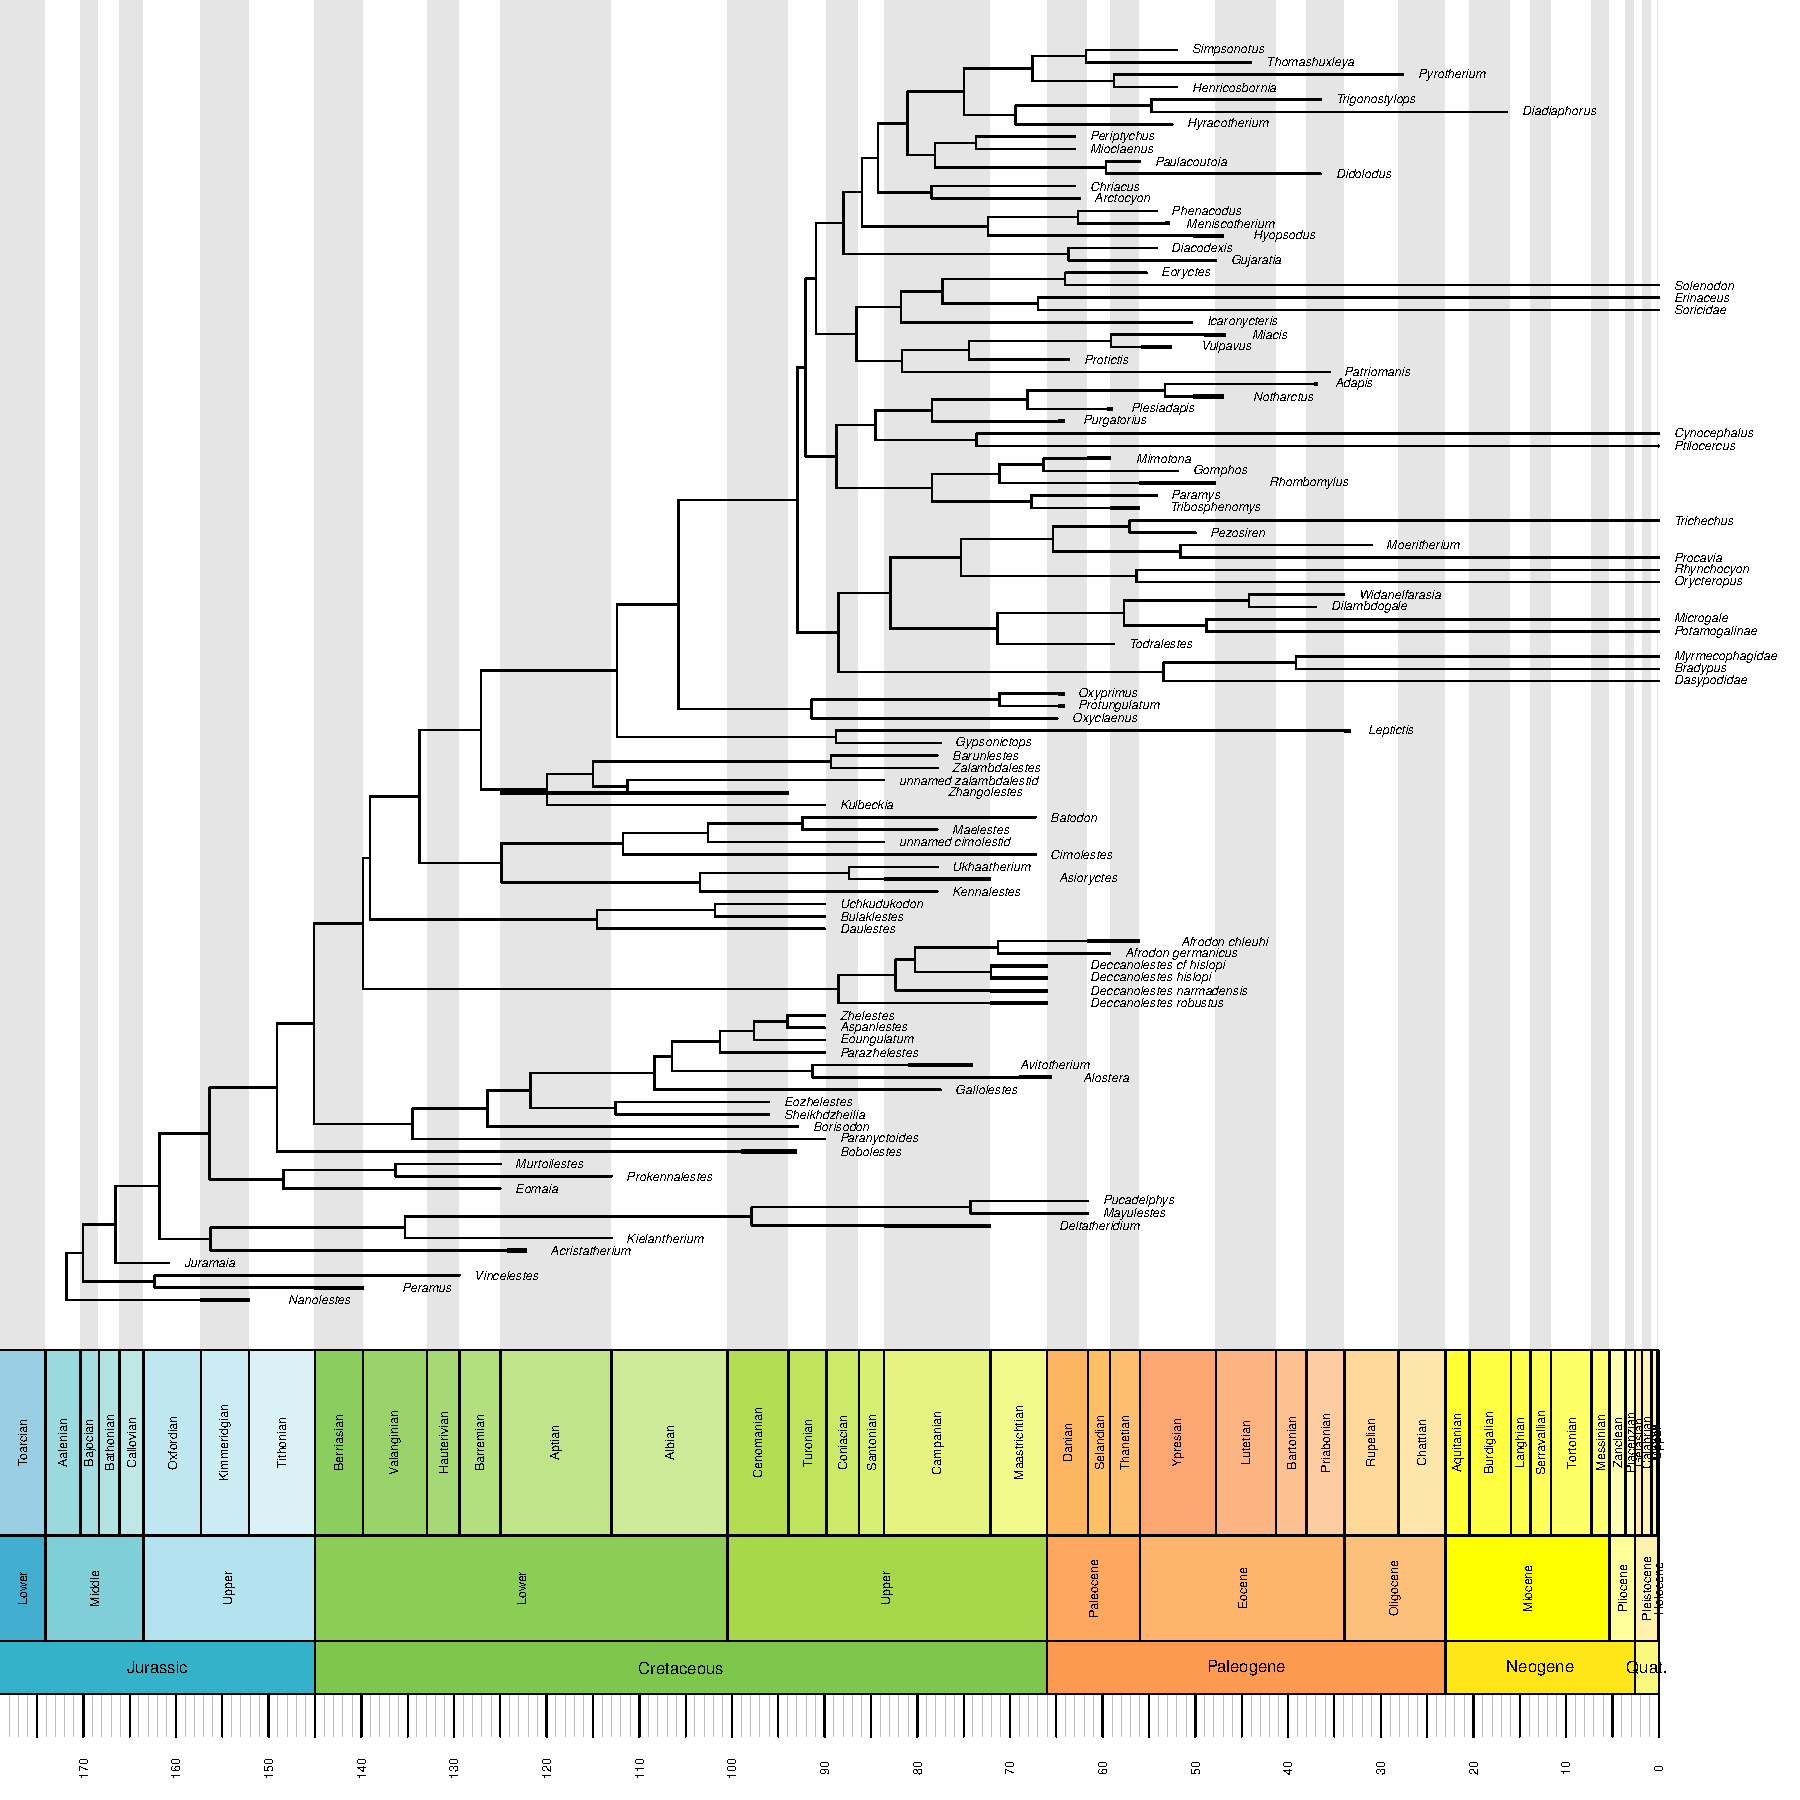
\includegraphics[width=1\linewidth, height=1\textheight, keepaspectratio]{figures/fig-tree-Beck2014-appendix.pdf}
    \caption[Beck2014.]
    {Phylogeny from Beck \& Lee (2014).}
    \label{figure:beck}
  \end{figure} 

\begin{figure}[!htbp]
    \centering
    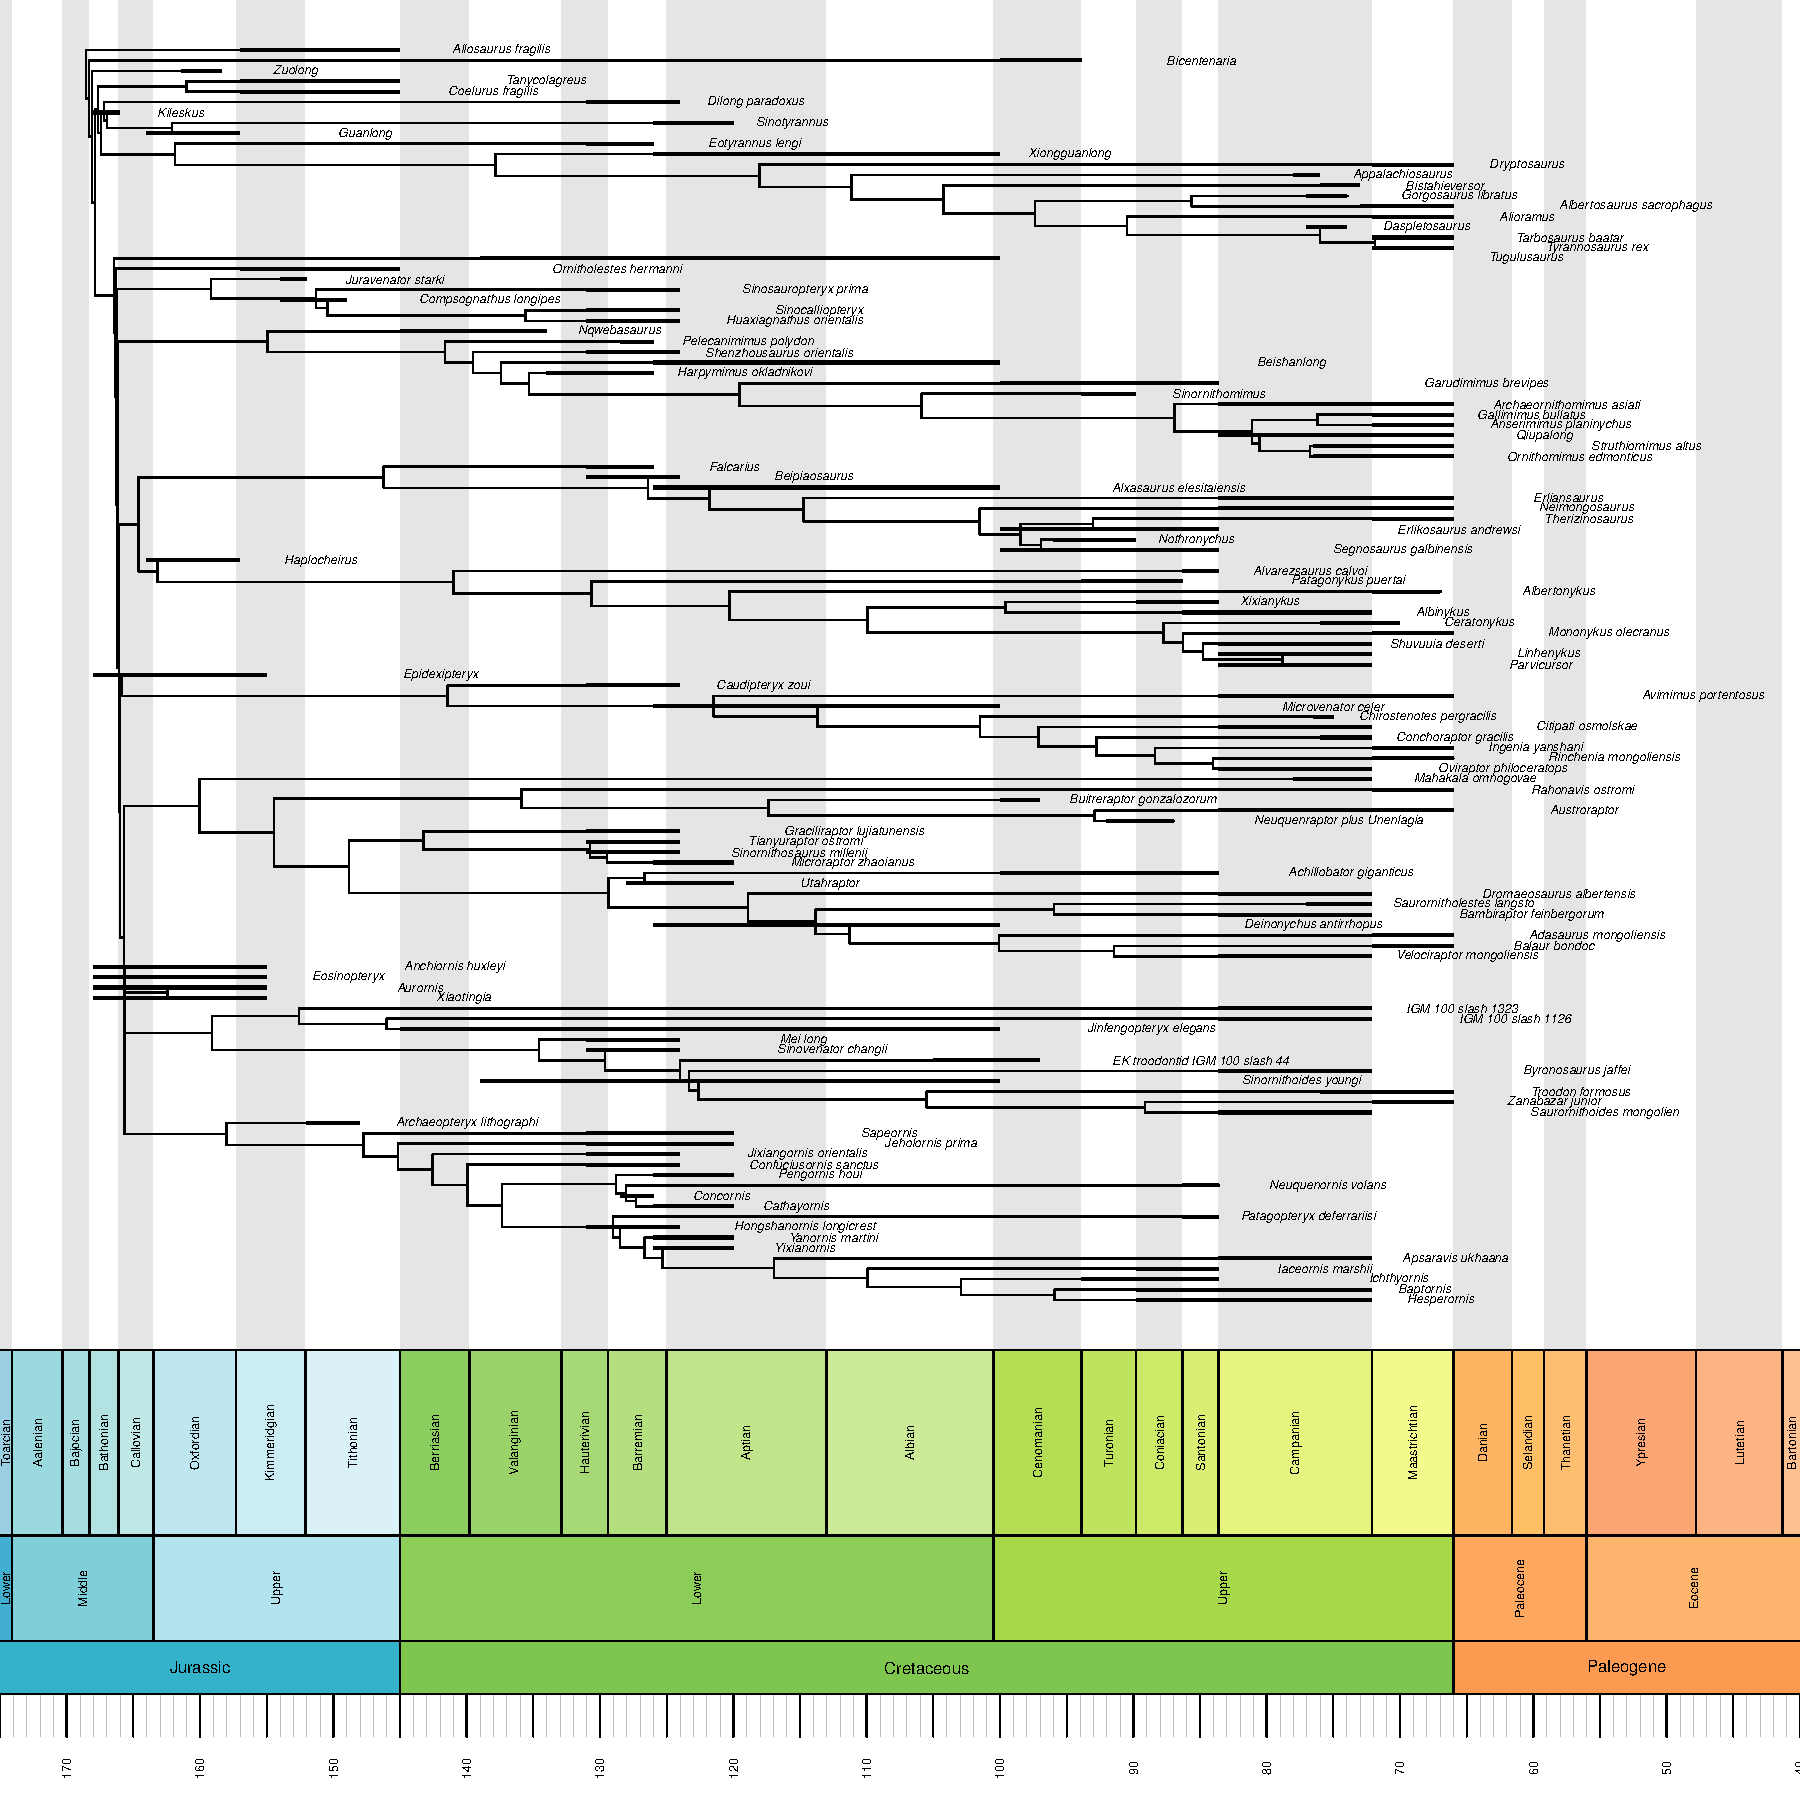
\includegraphics[width=1\linewidth, height=1\textheight, keepaspectratio]{figures/fig-tree-Brusatte2014-appendix.pdf}
    \caption[Brusatte2014.]
    {Phylogeny from Brusatte et al. (2014). This is one randomly selected tree from the time-scaled trees in the paper.}
    \label{figure:brusatte}
  \end{figure} 

\begin{figure}[!htbp]
    \centering
    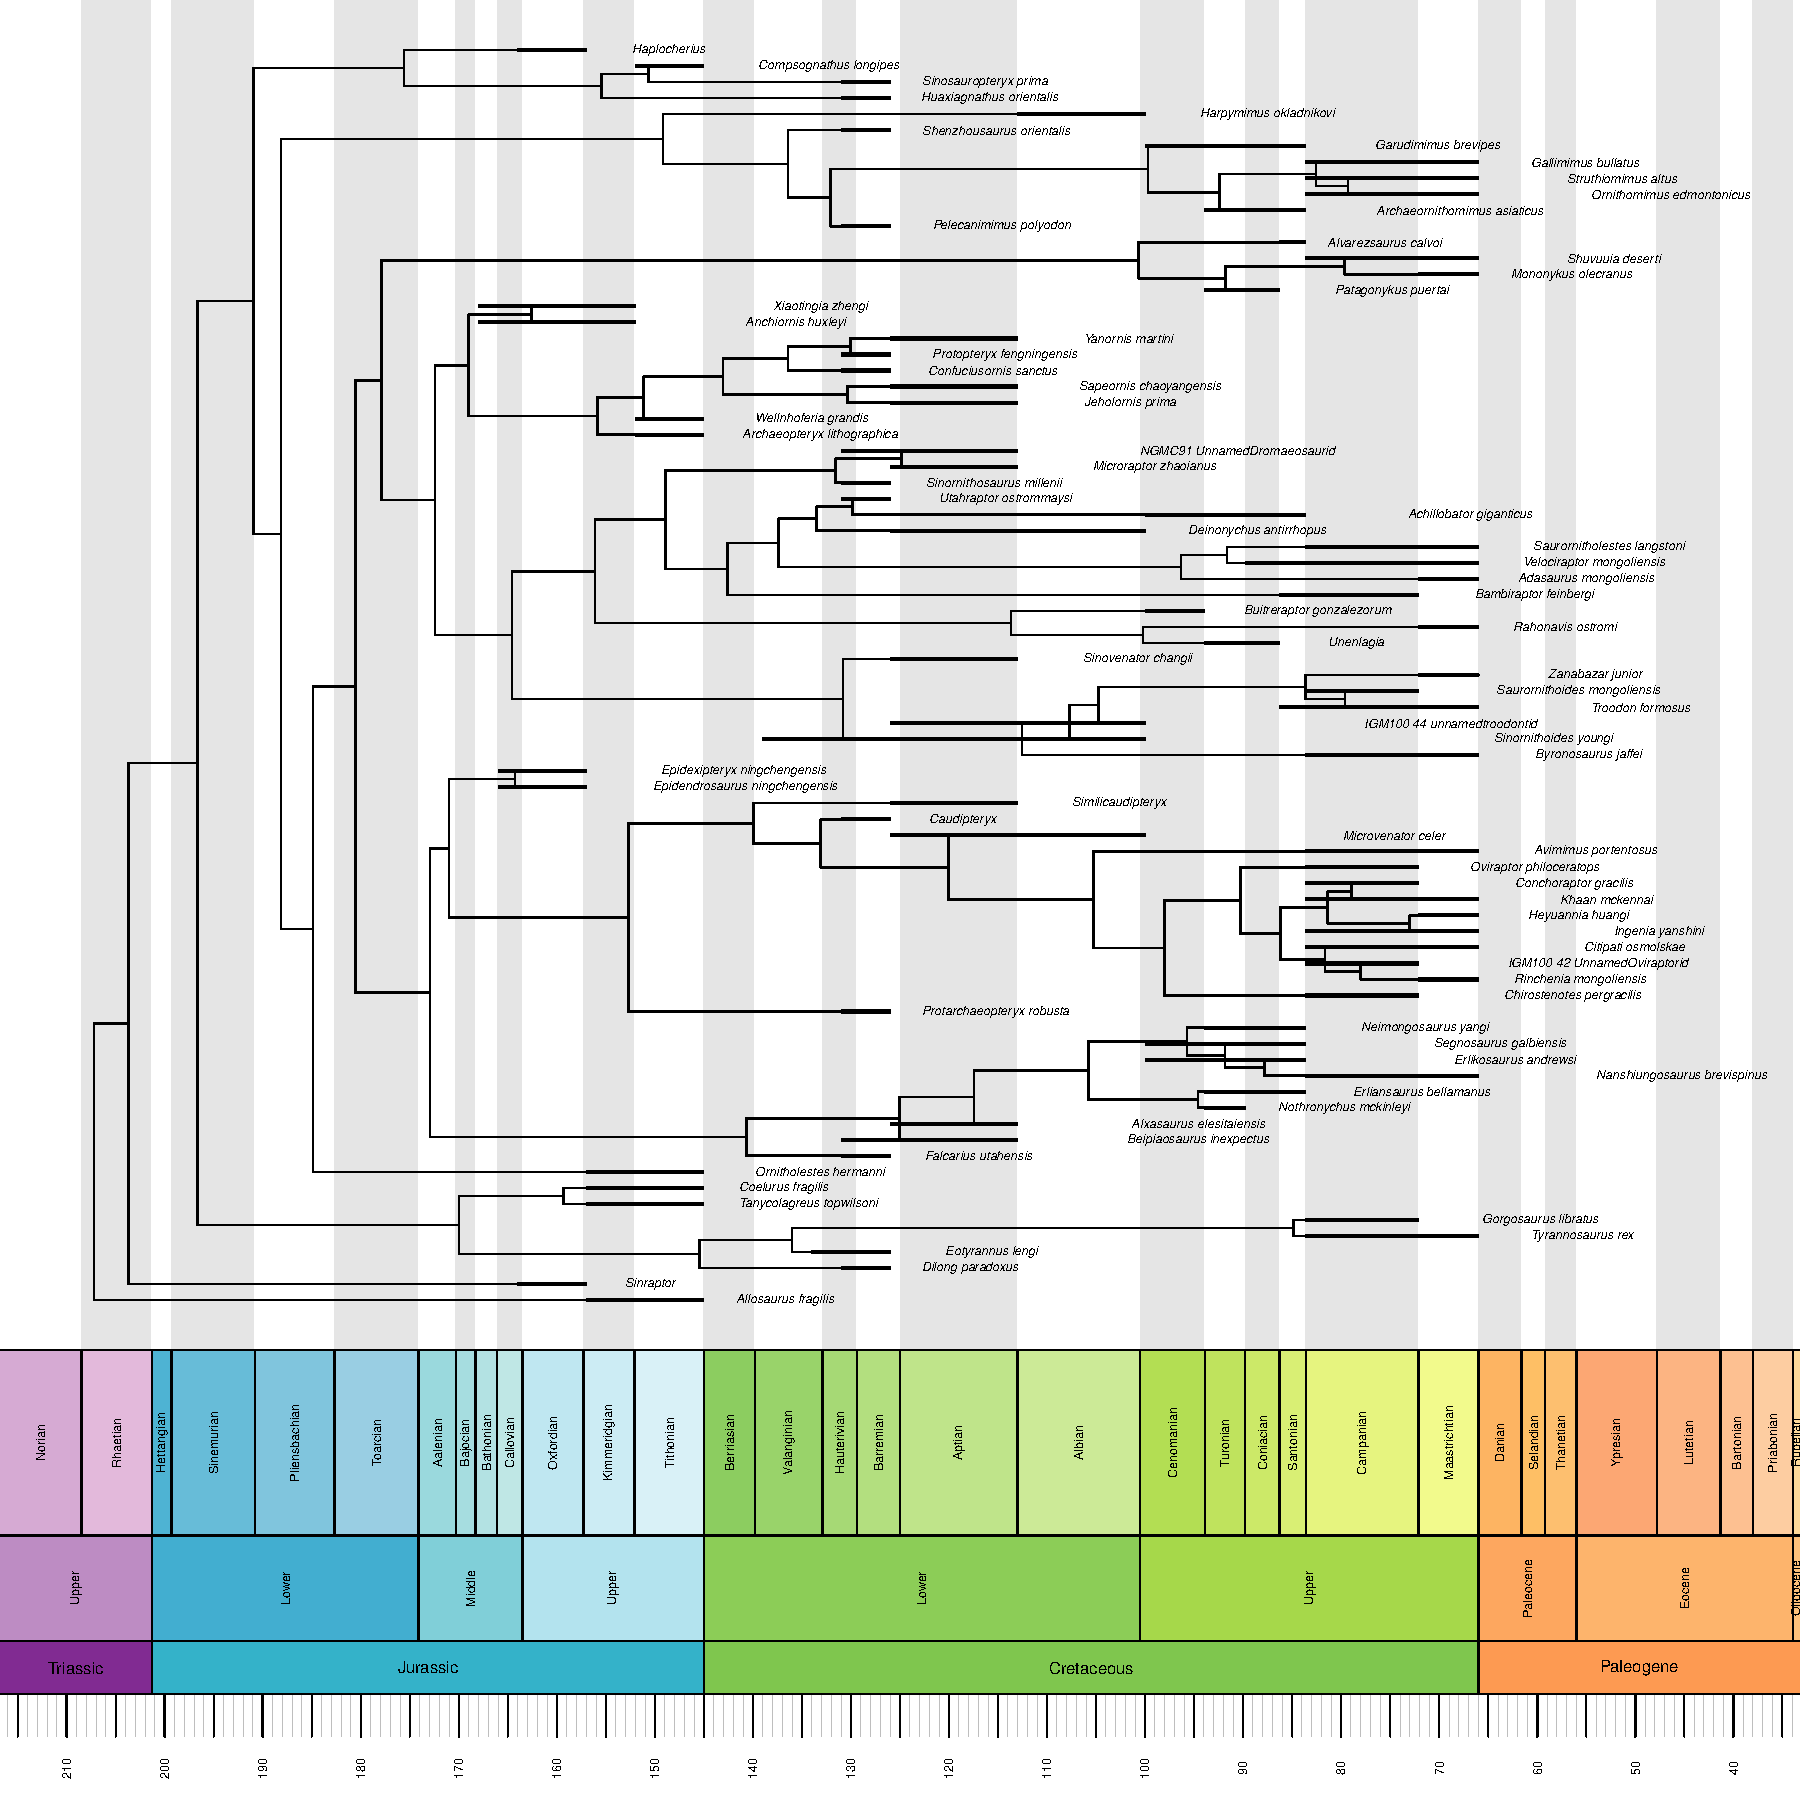
\includegraphics[width=1\linewidth, height=1\textheight, keepaspectratio]{figures/fig-tree-Bapst2016-appendix.pdf}
    \caption[Bapst2016.]
    {Phylogeny from Bapst et al. (2016). This is the maximum clade credibility tree.}
    \label{figure:bapst}
  \end{figure} 

\begin{figure}[!htbp]
    \centering
    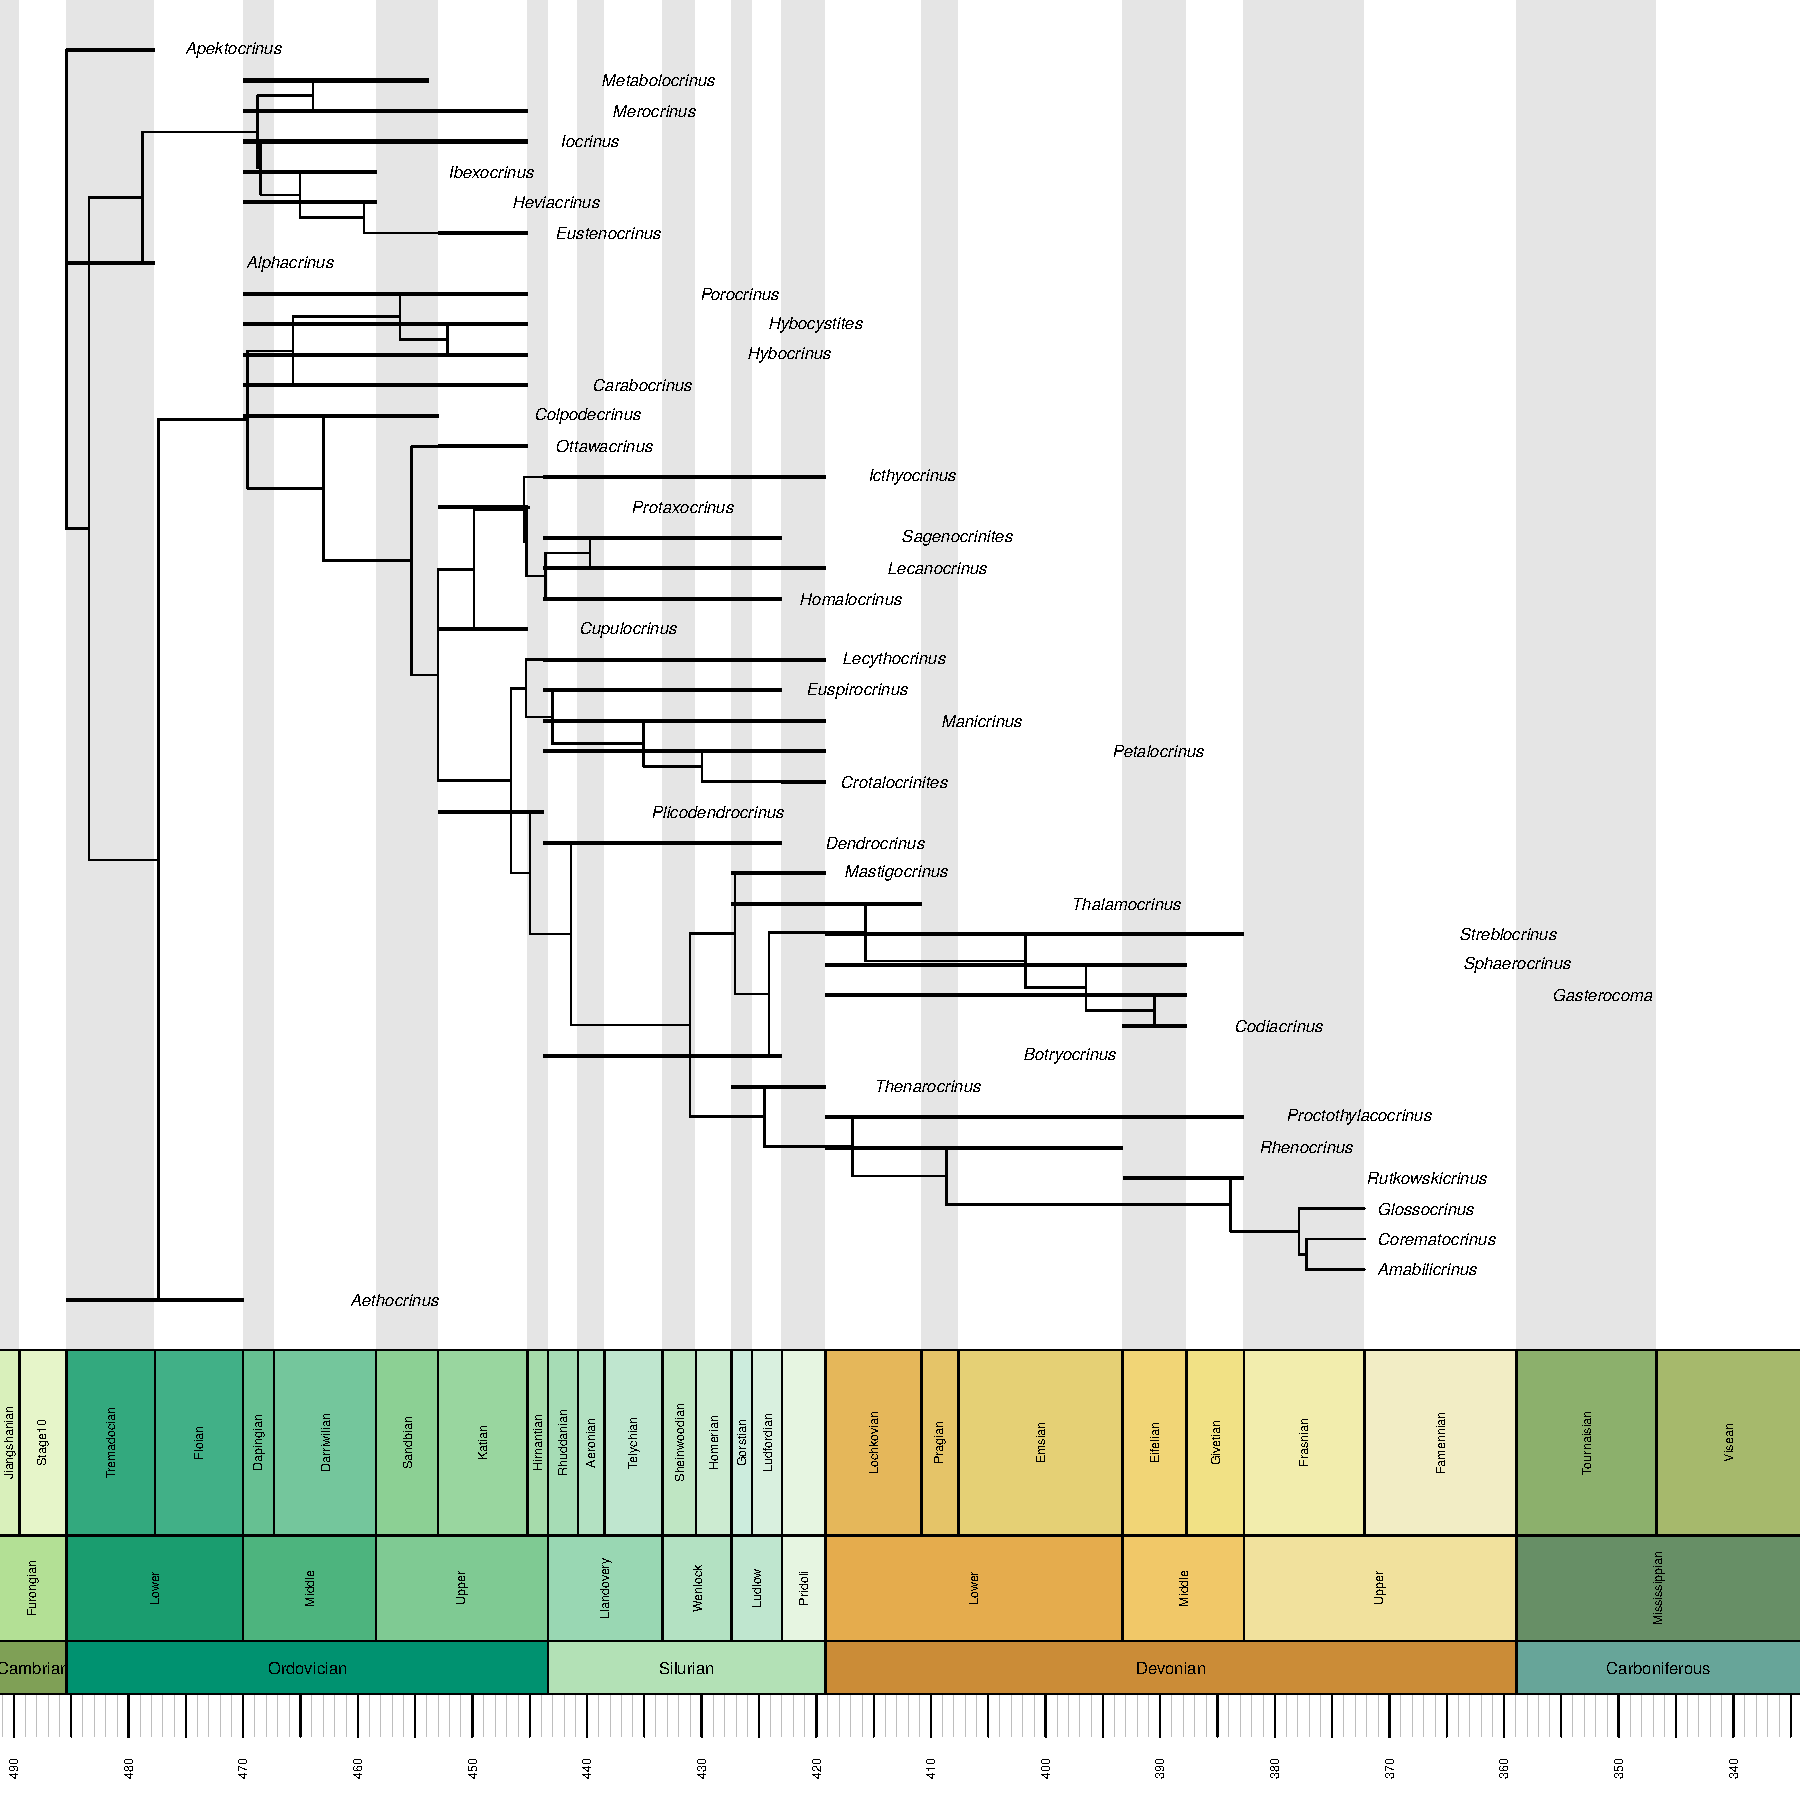
\includegraphics[width=1\linewidth, height=1\textheight, keepaspectratio]{figures/fig-tree-Wright2017-appendix.pdf}
    \caption[Wright2017.]
    {This is the maximum clade credibility tree from Wright (2017).}
    \label{figure:wright}
  \end{figure}  

\newpage
\section{Appendix S2: Additional tables and figures}

% DTT figures
  \begin{figure}[!htbp]
    \centering
    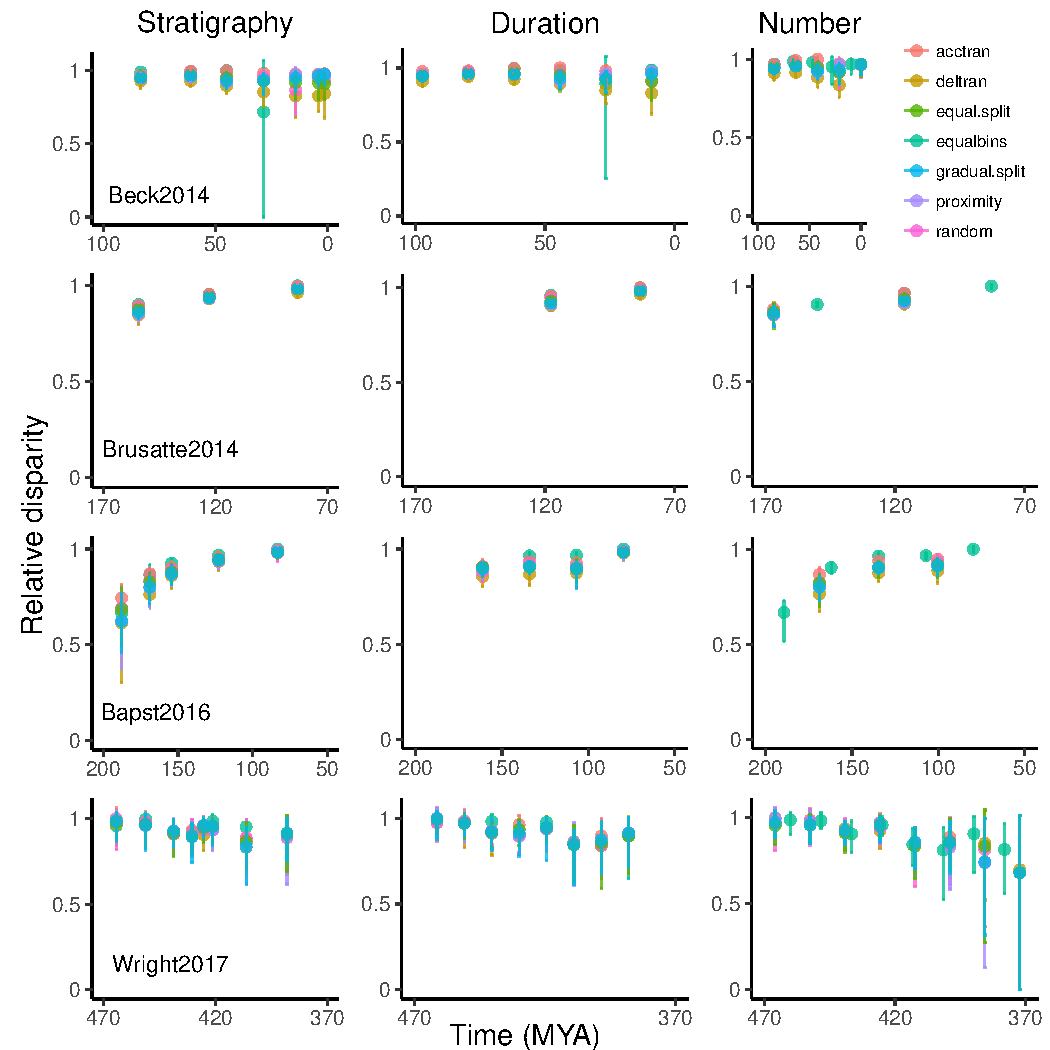
\includegraphics[width=1\linewidth, height=1\textheight, keepaspectratio]{figures/fig-dtt-epoch-appendix.pdf}
    \caption[Relative disparity through time for four example datasets.]
    {Median bootstrapped disparities were calculated using time binning and time-slicing approaches. 
    Relative disparities (median bootstrapped disparity divided by the maximum median bootstrapped disparity for a dataset and analysis method) are presented so they can be compared across datasets/methods. 
    Stratigraphy uses unequal time bins or non-equidistant slices, where the width of the bin, or the interval between slices, is equivalent to stratigraphic epochs. 
    Duration uses equal time bins or equidistant slices, where the width of the bin, or the interval between slices, is the average duration of stratigraphic epochs in the time frame of the dataset. 
    Number uses equal time bins or equidistant slices, where the number of bins, or the number of slices, is the average number of stratigraphic epochs in the time frame of the dataset. 
    In all cases, time bin disparities are plotted at the midpoint of the bin, and error bars represent the 95\% confidence intervals around the bootstrapped median disparity.
    The four dataset names are on the first plot for each dataset (Table \ref{table:datasets}).}
    \label{figure:dtt2}
  \end{figure}  

  \begin{figure}[!htbp]
    \centering
    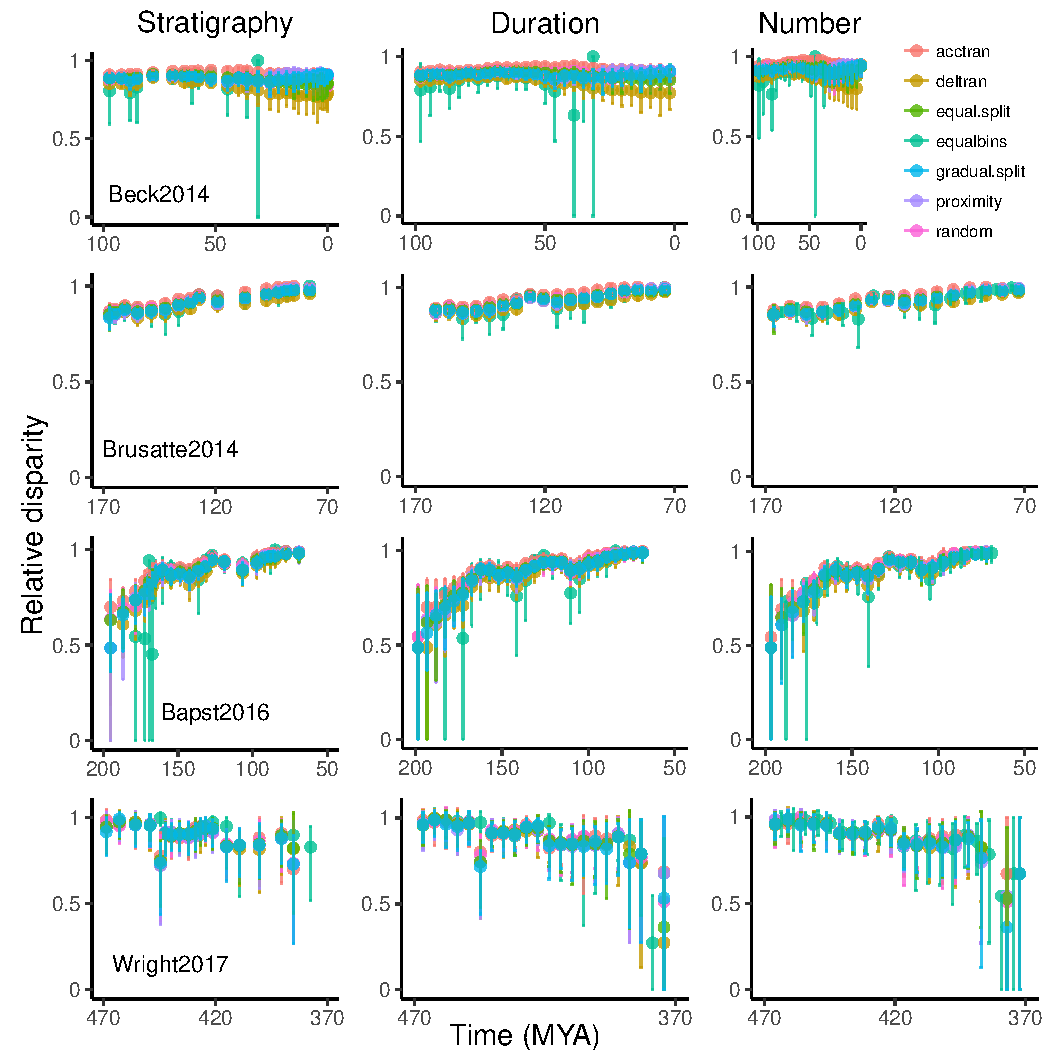
\includegraphics[width=1\linewidth, height=1\textheight, keepaspectratio]{figures/fig-dtt-age-appendix.pdf}
    \caption[Relative disparity through time for four example datasets.]
    {Median bootstrapped disparities were calculated using time binning and time-slicing approaches. 
    Relative disparities (median bootstrapped disparity divided by the maximum median bootstrapped disparity for a dataset and analysis method) are presented so they can be compared across datasets/methods. 
    Stratigraphy uses unequal time bins or non-equidistant slices, where the width of the bin, or the interval between slices, is equivalent to stratigraphic ages. 
    Duration uses equal time bins or equidistant slices, where the width of the bin, or the interval between slices, is the average duration of stratigraphic ages in the time frame of the dataset. 
    Number uses equal time bins or equidistant slices, where the number of bins, or the number of slices, is the average number of stratigraphic ages in the time frame of the dataset. 
    In all cases, time bin disparities are plotted at the midpoint of the bin, and error bars represent the 95\% confidence intervals around the bootstrapped median disparity.
    The four dataset names are on the first plot for each dataset (Table \ref{table:datasets}).}
    \label{figure:dtt3}
  \end{figure}  

% Wilcoxon results table
  % latex table generated in R 3.4.2 by xtable 1.8-2 package
% Fri Dec  8 17:06:33 2017
\begin{table}[!htbp]
\centering
\begin{tabular}{lllccc}
  \hline
\textbf{Dataset} & \textbf{Period} & \textbf{Model} & \textbf{Stratigraphy} & \textbf{Duration} & \textbf{Number} \\ 
  \hline
Beck2014 & Age & acctran & 39*** & 76 & 11 \\ 
  Beck2014 & Age & deltran & 188*** & 194*** & 171 \\ 
  Beck2014 & Age & equal.split & 91 & 119*** & 47 \\ 
  Beck2014 & Age & gradual.split & 111 & 115*** & 65*** \\ 
  Beck2014 & Age & proximity & 105 & 83 & 68*** \\ 
  Beck2014 & Age & random & 97 & 104*** & 45 \\ 
  Beck2014 & Epoch & acctran & 14 & 10 & 14 \\ 
  Beck2014 & Epoch & deltran & 21 & 45*** & 41*** \\ 
  Beck2014 & Epoch & equal.split & 21 & 40*** & 42*** \\ 
  Beck2014 & Epoch & gradual.split & 21 & 39 & 43*** \\ 
  Beck2014 & Epoch & proximity & 21 & 36 & 32 \\ 
  Beck2014 & Epoch & random & 21 & 37 & 45*** \\ 
  Brusatte2014 & Age & acctran & 27*** & 28 & 28*** \\ 
  Brusatte2014 & Age & deltran & 27*** & 29 & 31*** \\ 
  Brusatte2014 & Age & equal.split & 28*** & 58*** & 50*** \\ 
  Brusatte2014 & Age & gradual.split & 28*** & 61*** & 52*** \\ 
  Brusatte2014 & Age & proximity & 27*** & 31 & 28*** \\ 
  Brusatte2014 & Age & random & 27*** & 27 & 27*** \\ 
  Brusatte2014 & Epoch & acctran & 0 & 5*** & 5 \\ 
  Brusatte2014 & Epoch & deltran & 0 & 5*** & 5 \\ 
  Brusatte2014 & Epoch & equal.split & 3 & 6 & 6 \\ 
  Brusatte2014 & Epoch & gradual.split & 3 & 6 & 6 \\ 
  Brusatte2014 & Epoch & proximity & 0 & 5*** & 5 \\ 
  Brusatte2014 & Epoch & random & 0 & 5*** & 5 \\ 
  Bapst2016 & Age & acctran & 45*** & 47 & 72*** \\ 
  Bapst2016 & Age & deltran & 55*** & 46 & 78*** \\ 
  Bapst2016 & Age & equal.split & 93 & 147*** & 153 \\ 
  Bapst2016 & Age & gradual.split & 93 & 153 & 165 \\ 
  Bapst2016 & Age & proximity & 57*** & 47 & 75*** \\ 
  Bapst2016 & Age & random & 57*** & 48 & 81*** \\ 
  Bapst2016 & Epoch & acctran & 2 & 0*** & 8 \\ 
  Bapst2016 & Epoch & deltran & 2 & 0*** & 9 \\ 
  Bapst2016 & Epoch & equal.split & 4 & 6 & 13 \\ 
  Bapst2016 & Epoch & gradual.split & 4 & 6 & 12 \\ 
  Bapst2016 & Epoch & proximity & 2 & 0*** & 8 \\ 
  Bapst2016 & Epoch & random & 2 & 1*** & 8 \\ 
  Wright2017 & Age & acctran & 146*** & 146 & 84 \\ 
  Wright2017 & Age & deltran & 162*** & 138 & 101 \\ 
  Wright2017 & Age & equal.split & 151*** & 160 & 105 \\ 
  Wright2017 & Age & gradual.split & 152*** & 155 & 116 \\ 
  Wright2017 & Age & proximity & 160*** & 175*** & 101 \\ 
  Wright2017 & Age & random & 150*** & 147 & 111 \\ 
  Wright2017 & Epoch & acctran & 25 & 20 & 18 \\ 
  Wright2017 & Epoch & deltran & 27 & 26 & 25 \\ 
  Wright2017 & Epoch & equal.split & 29 & 30 & 25 \\ 
  Wright2017 & Epoch & gradual.split & 28 & 29 & 21 \\ 
  Wright2017 & Epoch & proximity & 23 & 28 & 18 \\ 
  Wright2017 & Epoch & random & 28 & 23 & 17 \\ 
   \hline
\end{tabular}
\caption{Wilcoxon results for appendix} 
\end{table}
 
  \label{table:wilcox2}  

% disparity peaks figures
\begin{figure}[!htbp]
    \centering
    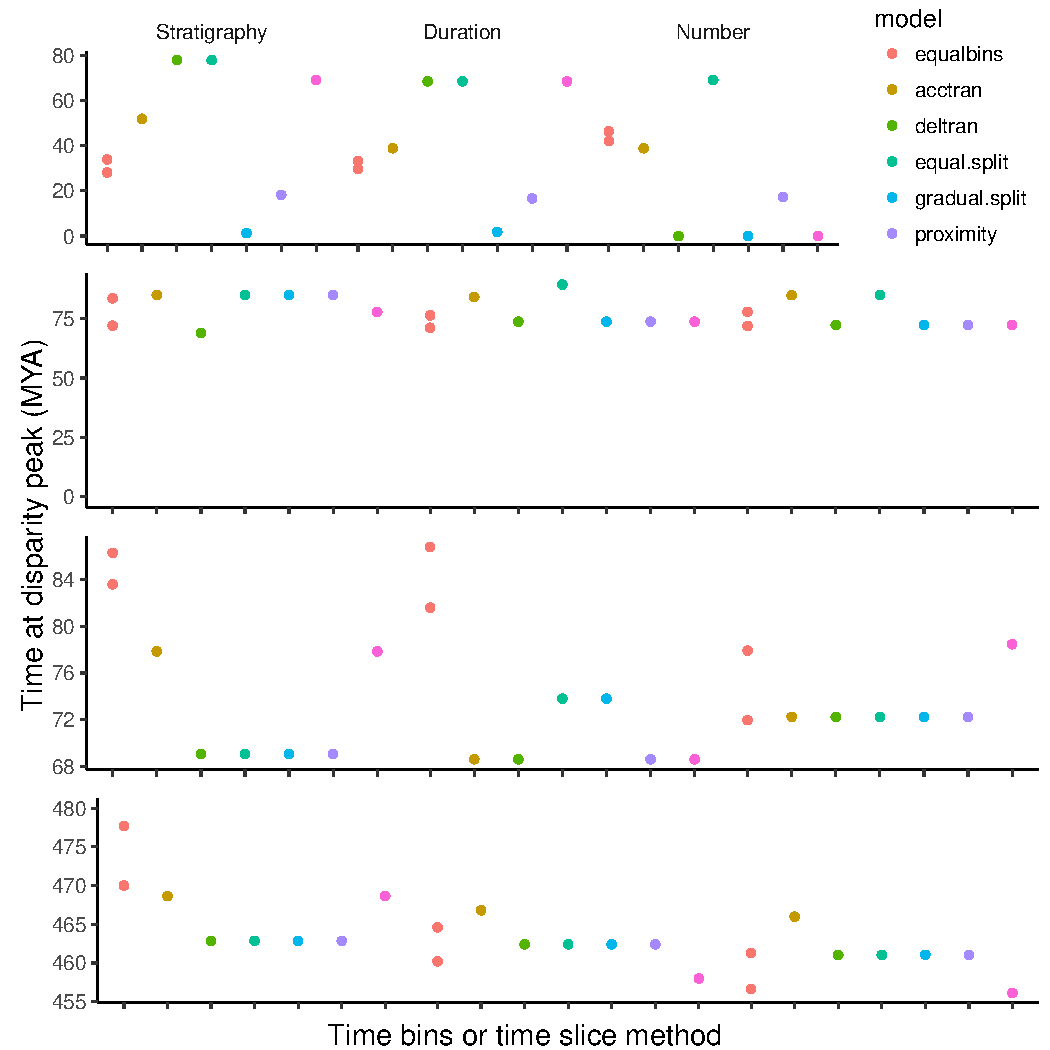
\includegraphics[width=1\linewidth, height=1\textheight, keepaspectratio]{figures/fig-peaks-epoch-appendix.pdf}
    \caption[Timing of peak disparity for four example datasets.]
    {Median bootstrapped disparities were calculated using time binning and time-slicing approaches. 
    Stratigraphy uses unequal time bins or non-equidistant slices, where the width of the bin, or the interval between slices, is equivalent to stratigraphic epochs. 
    Duration uses equal time bins or equidistant slices, where the width of the bin, or the interval between slices, is the average duration of stratigraphic epochs in the time frame of the dataset. 
    Number uses equal time bins or equidistant slices, where the number of bins, or the number of slices, is the average number of stratigraphic epochs in the time frame of the dataset. 
    For time bins there are two points indicating the maximum and minimum ages of the time bin within which peak disparities appeared.
    The four dataset names are on the first plot for each dataset (Table \ref{table:datasets}).}
    \label{figure:peak2}
  \end{figure}

\begin{figure}[!htbp]
    \centering
    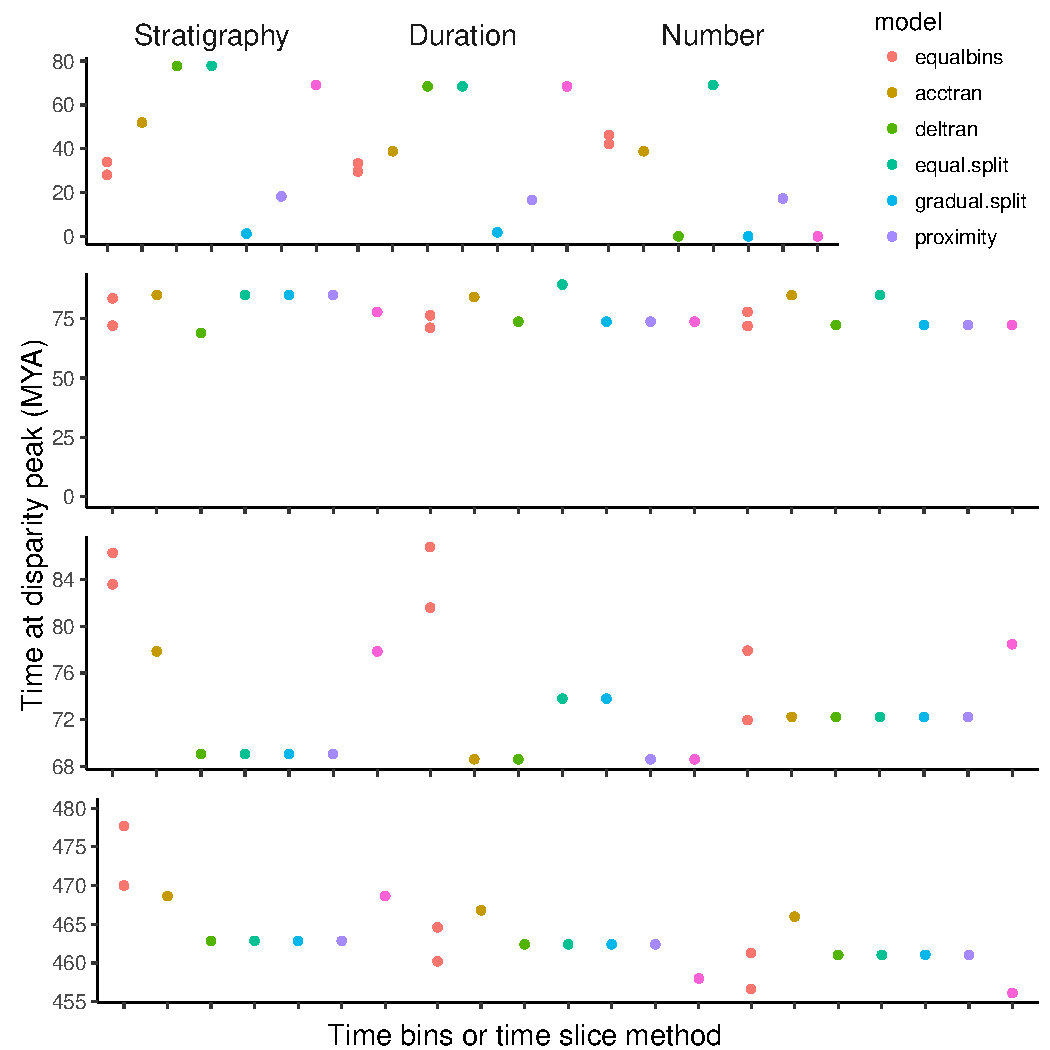
\includegraphics[width=1\linewidth, height=1\textheight, keepaspectratio]{figures/fig-peaks-age-appendix.pdf}
    \caption[Timing of peak disparity for four example datasets.]
    {Median bootstrapped disparities were calculated using time binning and time-slicing approaches. 
    Stratigraphy uses unequal time bins or non-equidistant slices, where the width of the bin, or the interval between slices, is equivalent to stratigraphic ages. 
    Duration uses equal time bins or equidistant slices, where the width of the bin, or the interval between slices, is the average duration of stratigraphic ages in the time frame of the dataset. 
    Number uses equal time bins or equidistant slices, where the number of bins, or the number of slices, is the average number of stratigraphic ages in the time frame of the dataset. 
    For time bins there are two points indicating the maximum and minimum ages of the time bin within which peak disparities appeared.
    The four dataset names are on the first plot for each dataset (Table 1).}
    \label{figure:peak3}
  \end{figure}

% Extinction figures


% Full results
\begin{landscape}
  % latex table generated in R 3.4.3 by xtable 1.8-2 package
% Thu Dec 21 15:01:42 2017
\begin{longtable}{llllrrrrrrr}
  \hline
stratigraphy & bin\_type & model & subsets & n & obs & bs.median & 2.5\% & 25\% & 75\% & 97.5\% \\ 
  \hline
Ages & stratigraphy & equalbins & 477.7 - 470 & 14.00 & 2.27 & 2.12 & 1.96 & 2.06 & 2.17 & 2.23 \\ 
   &  &  & 470 - 467.3 & 14.00 & 2.13 & 2.00 & 1.79 & 1.93 & 2.06 & 2.16 \\ 
   &  &  & 467.3 - 458.4 & 15.00 & 2.19 & 2.07 & 1.85 & 2.01 & 2.11 & 2.16 \\ 
   &  &  & 458.4 - 453 & 18.00 & 2.17 & 2.06 & 1.89 & 2.00 & 2.11 & 2.15 \\ 
   &  &  & 453 - 445.2 & 18.00 & 2.14 & 2.03 & 1.89 & 2.00 & 2.07 & 2.13 \\ 
   &  &  & 445.2 - 443.8 & 22.00 & 2.20 & 2.11 & 2.02 & 2.07 & 2.14 & 2.18 \\ 
   &  &  & 443.8 - 440.8 & 14.00 & 2.06 & 1.93 & 1.78 & 1.87 & 1.97 & 2.04 \\ 
   &  &  & 440.8 - 438.5 & 11.00 & 2.10 & 1.93 & 1.69 & 1.83 & 2.00 & 2.09 \\ 
   &  &  & 438.5 - 433.4 & 11.00 & 2.11 & 1.92 & 1.69 & 1.84 & 1.98 & 2.06 \\ 
   &  &  & 433.4 - 430.5 & 11.00 & 2.09 & 1.92 & 1.63 & 1.83 & 1.98 & 2.04 \\ 
   &  &  & 430.5 - 427.4 & 14.00 & 2.10 & 1.97 & 1.75 & 1.92 & 2.01 & 2.07 \\ 
   &  &  & 427.4 - 425.6 & 14.00 & 2.11 & 1.96 & 1.79 & 1.93 & 2.03 & 2.10 \\ 
   &  &  & 425.6 - 423 & 16.00 & 2.12 & 1.98 & 1.87 & 1.95 & 2.04 & 2.09 \\ 
   &  &  & 423 - 419.2 & 19.00 & 2.16 & 2.05 & 1.96 & 2.03 & 2.09 & 2.13 \\ 
   &  &  & 419.2 - 410.8 & 16.00 & 2.13 & 2.00 & 1.86 & 1.95 & 2.06 & 2.11 \\ 
   &  &  & 410.8 - 407.6 & 7.00 & 2.05 & 1.77 & 1.15 & 1.68 & 1.87 & 1.97 \\ 
   &  &  & 407.6 - 393.3 & 8.00 & 1.97 & 1.78 & 1.29 & 1.64 & 1.85 & 1.97 \\ 
   &  &  & 393.3 - 387.7 & 8.00 & 2.11 & 1.86 & 1.49 & 1.74 & 1.94 & 2.05 \\ 
   &  &  & 387.7 - 382.7 & 7.00 & 2.16 & 1.90 & 1.34 & 1.76 & 1.98 & 2.06 \\ 
   &  &  & 382.7 - 372.2 & 8.00 & 1.93 & 1.75 & 1.10 & 1.57 & 1.84 & 2.01 \\ 
   &  & acctran & 473.85 & 3.00 & 1.73 & 1.18 & 0.00 & 0.92 & 1.36 & 1.73 \\ 
   &  &  & 468.65 & 12.00 & 2.24 & 2.08 & 1.73 & 2.00 & 2.13 & 2.21 \\ 
   &  &  & 462.85 & 12.00 & 2.20 & 2.03 & 1.83 & 1.96 & 2.09 & 2.18 \\ 
   &  &  & 455.7 & 10.00 & 2.24 & 2.04 & 1.73 & 1.95 & 2.08 & 2.18 \\ 
   &  &  & 449.1 & 13.00 & 2.18 & 2.03 & 1.88 & 1.97 & 2.08 & 2.15 \\ 
   &  &  & 444.5 & 6.00 & 1.95 & 1.64 & 1.23 & 1.53 & 1.76 & 1.93 \\ 
   &  &  & 442.3 & 12.00 & 2.09 & 1.92 & 1.73 & 1.85 & 1.97 & 2.05 \\ 
   &  &  & 439.65 & 12.00 & 2.05 & 1.88 & 1.62 & 1.81 & 1.95 & 2.04 \\ 
   &  &  & 435.95 & 12.00 & 2.05 & 1.86 & 1.67 & 1.79 & 1.97 & 2.05 \\ 
   &  &  & 431.95 & 12.00 & 2.04 & 1.88 & 1.60 & 1.82 & 1.95 & 2.01 \\ 
   &  &  & 428.95 & 12.00 & 2.16 & 1.99 & 1.77 & 1.94 & 2.05 & 2.10 \\ 
   &  &  & 426.5 & 15.00 & 2.14 & 2.01 & 1.83 & 1.95 & 2.05 & 2.11 \\ 
   &  &  & 424.3 & 15.00 & 2.15 & 2.01 & 1.88 & 1.95 & 2.05 & 2.12 \\ 
   &  &  & 421.1 & 11.00 & 2.13 & 1.96 & 1.72 & 1.88 & 2.02 & 2.09 \\ 
   &  &  & 415 & 8.00 & 2.00 & 1.78 & 1.42 & 1.68 & 1.85 & 1.95 \\ 
   &  &  & 409.2 & 7.00 & 2.02 & 1.77 & 1.32 & 1.61 & 1.86 & 1.98 \\ 
   &  &  & 400.45 & 7.00 & 2.11 & 1.86 & 1.32 & 1.74 & 1.95 & 2.11 \\ 
   &  &  & 390.5 & 7.00 & 2.16 & 1.92 & 1.31 & 1.80 & 1.98 & 2.08 \\ 
   &  &  & 385.2 & 4.00 & 2.07 & 1.48 & 0.57 & 1.15 & 1.86 & 2.07 \\ 
   &  &  & 377.45 & 2.00 & 1.14 & 0.00 & 0.00 & 0.00 & 1.14 & 1.14 \\ 
   &  & deltran & 473.85 & 3.00 & 1.61 & 1.22 & 0.00 & 0.76 & 1.24 & 1.61 \\ 
   &  &  & 468.65 & 12.00 & 2.17 & 1.99 & 1.77 & 1.93 & 2.07 & 2.16 \\ 
   &  &  & 462.85 & 12.00 & 2.24 & 2.07 & 1.86 & 2.01 & 2.13 & 2.20 \\ 
   &  &  & 455.7 & 10.00 & 2.27 & 2.06 & 1.81 & 2.00 & 2.12 & 2.18 \\ 
   &  &  & 449.1 & 13.00 & 2.17 & 2.02 & 1.71 & 1.96 & 2.07 & 2.15 \\ 
   &  &  & 444.5 & 5.00 & 1.81 & 1.53 & 1.12 & 1.32 & 1.63 & 1.81 \\ 
   &  &  & 442.3 & 12.00 & 2.09 & 1.93 & 1.71 & 1.87 & 2.00 & 2.08 \\ 
   &  &  & 439.65 & 12.00 & 2.08 & 1.93 & 1.71 & 1.87 & 1.98 & 2.06 \\ 
   &  &  & 435.95 & 12.00 & 2.08 & 1.92 & 1.69 & 1.85 & 1.97 & 2.07 \\ 
   &  &  & 431.95 & 12.00 & 2.09 & 1.92 & 1.72 & 1.86 & 1.97 & 2.05 \\ 
   &  &  & 428.95 & 12.00 & 2.04 & 1.89 & 1.67 & 1.82 & 1.95 & 2.03 \\ 
   &  &  & 426.5 & 15.00 & 2.04 & 1.91 & 1.69 & 1.82 & 1.98 & 2.04 \\ 
   &  &  & 424.3 & 15.00 & 2.09 & 1.95 & 1.77 & 1.90 & 1.98 & 2.06 \\ 
   &  &  & 421.1 & 11.00 & 2.13 & 1.94 & 1.74 & 1.86 & 1.98 & 2.08 \\ 
   &  &  & 415 & 8.00 & 1.98 & 1.76 & 1.39 & 1.64 & 1.84 & 1.94 \\ 
   &  &  & 409.2 & 7.00 & 2.02 & 1.73 & 1.28 & 1.64 & 1.83 & 1.93 \\ 
   &  &  & 400.45 & 7.00 & 2.02 & 1.72 & 1.19 & 1.63 & 1.87 & 1.96 \\ 
   &  &  & 390.5 & 7.00 & 2.17 & 1.87 & 1.42 & 1.73 & 1.98 & 2.11 \\ 
   &  &  & 385.2 & 4.00 & 2.17 & 1.73 & 0.94 & 1.12 & 1.87 & 2.17 \\ 
   &  &  & 377.45 & 1.00 &  &  &  &  &  &  \\ 
   &  & random & 473.85 & 3.00 & 1.61 & 1.24 & 0.00 & 0.76 & 1.61 & 1.61 \\ 
   &  &  & 468.65 & 12.00 & 2.23 & 2.06 & 1.82 & 2.00 & 2.10 & 2.19 \\ 
   &  &  & 462.85 & 12.00 & 2.20 & 2.01 & 1.79 & 1.95 & 2.10 & 2.16 \\ 
   &  &  & 455.7 & 10.00 & 2.23 & 2.02 & 1.76 & 1.92 & 2.09 & 2.18 \\ 
   &  &  & 449.1 & 13.00 & 2.18 & 2.03 & 1.75 & 1.95 & 2.08 & 2.15 \\ 
   &  &  & 444.5 & 5.00 & 1.90 & 1.58 & 0.83 & 1.35 & 1.74 & 1.90 \\ 
   &  &  & 442.3 & 12.00 & 2.09 & 1.94 & 1.71 & 1.88 & 1.99 & 2.06 \\ 
   &  &  & 439.65 & 12.00 & 2.08 & 1.91 & 1.63 & 1.84 & 1.99 & 2.07 \\ 
   &  &  & 435.95 & 12.00 & 2.05 & 1.89 & 1.72 & 1.83 & 1.96 & 2.04 \\ 
   &  &  & 431.95 & 12.00 & 2.04 & 1.86 & 1.67 & 1.80 & 1.95 & 2.05 \\ 
   &  &  & 428.95 & 12.00 & 2.11 & 1.96 & 1.65 & 1.88 & 2.00 & 2.08 \\ 
   &  &  & 426.5 & 15.00 & 2.09 & 1.93 & 1.78 & 1.90 & 1.99 & 2.07 \\ 
   &  &  & 424.3 & 15.00 & 2.09 & 1.97 & 1.82 & 1.91 & 2.03 & 2.09 \\ 
   &  &  & 421.1 & 11.00 & 2.12 & 1.93 & 1.77 & 1.88 & 1.99 & 2.08 \\ 
   &  &  & 415 & 8.00 & 2.00 & 1.79 & 1.35 & 1.72 & 1.86 & 1.96 \\ 
   &  &  & 409.2 & 7.00 & 2.02 & 1.77 & 1.35 & 1.67 & 1.86 & 1.97 \\ 
   &  &  & 400.45 & 7.00 & 2.11 & 1.82 & 1.43 & 1.74 & 1.93 & 2.08 \\ 
   &  &  & 390.5 & 7.00 & 2.17 & 1.87 & 1.46 & 1.75 & 2.00 & 2.09 \\ 
   &  &  & 385.2 & 4.00 & 2.07 & 1.55 & 0.57 & 1.44 & 1.87 & 2.07 \\ 
   &  &  & 377.45 & 2.00 & 1.14 & 0.00 & 0.00 & 0.00 & 1.14 & 1.14 \\ 
   &  & proximity & 473.85 & 3.00 & 1.61 & 1.22 & 0.00 & 0.76 & 1.24 & 1.61 \\ 
   &  &  & 468.65 & 12.00 & 2.17 & 1.99 & 1.67 & 1.92 & 2.06 & 2.17 \\ 
   &  &  & 462.85 & 12.00 & 2.24 & 2.07 & 1.83 & 2.01 & 2.12 & 2.19 \\ 
   &  &  & 455.7 & 10.00 & 2.23 & 2.03 & 1.76 & 1.95 & 2.09 & 2.19 \\ 
   &  &  & 449.1 & 13.00 & 2.18 & 2.03 & 1.80 & 1.95 & 2.08 & 2.15 \\ 
   &  &  & 444.5 & 5.00 & 1.81 & 1.53 & 0.80 & 1.29 & 1.63 & 1.81 \\ 
   &  &  & 442.3 & 12.00 & 2.08 & 1.93 & 1.66 & 1.87 & 1.99 & 2.06 \\ 
   &  &  & 439.65 & 12.00 & 2.08 & 1.94 & 1.71 & 1.86 & 2.00 & 2.08 \\ 
   &  &  & 435.95 & 12.00 & 2.05 & 1.91 & 1.65 & 1.84 & 1.97 & 2.08 \\ 
   &  &  & 431.95 & 12.00 & 2.04 & 1.88 & 1.67 & 1.79 & 1.95 & 2.06 \\ 
   &  &  & 428.95 & 12.00 & 2.04 & 1.89 & 1.63 & 1.80 & 1.95 & 2.04 \\ 
   &  &  & 426.5 & 15.00 & 2.09 & 1.92 & 1.80 & 1.89 & 1.98 & 2.07 \\ 
   &  &  & 424.3 & 15.00 & 2.14 & 2.01 & 1.86 & 1.96 & 2.04 & 2.10 \\ 
   &  &  & 421.1 & 11.00 & 2.13 & 1.94 & 1.69 & 1.87 & 2.03 & 2.08 \\ 
   &  &  & 415 & 8.00 & 1.98 & 1.75 & 1.43 & 1.69 & 1.85 & 1.94 \\ 
   &  &  & 409.2 & 7.00 & 2.03 & 1.78 & 1.33 & 1.66 & 1.86 & 1.98 \\ 
   &  &  & 400.45 & 7.00 & 2.02 & 1.77 & 1.24 & 1.68 & 1.90 & 1.99 \\ 
   &  &  & 390.5 & 7.00 & 2.16 & 1.89 & 1.55 & 1.82 & 1.97 & 2.07 \\ 
   &  &  & 385.2 & 4.00 & 2.07 & 1.54 & 0.57 & 1.46 & 1.86 & 2.07 \\ 
   &  &  & 377.45 & 2.00 & 1.14 & 0.00 & 0.00 & 0.00 & 1.14 & 1.14 \\ 
   &  & equal.split & 473.85 & 3.00 & 1.61 & 1.20 & 0.00 & 0.76 & 1.36 & 1.73 \\ 
   &  &  & 468.65 & 14.00 & 2.18 & 2.00 & 1.66 & 1.93 & 2.08 & 2.14 \\ 
   &  &  & 462.85 & 15.00 & 2.21 & 2.06 & 1.86 & 2.00 & 2.10 & 2.18 \\ 
   &  &  & 455.7 & 11.00 & 2.21 & 2.04 & 1.80 & 1.96 & 2.09 & 2.16 \\ 
   &  &  & 449.1 & 13.00 & 2.18 & 2.02 & 1.84 & 1.94 & 2.07 & 2.15 \\ 
   &  &  & 444.5 & 6.00 & 1.88 & 1.59 & 1.03 & 1.44 & 1.68 & 1.84 \\ 
   &  &  & 442.3 & 14.00 & 2.05 & 1.92 & 1.68 & 1.85 & 1.96 & 2.05 \\ 
   &  &  & 439.65 & 14.00 & 2.05 & 1.89 & 1.73 & 1.82 & 1.96 & 2.03 \\ 
   &  &  & 435.95 & 13.00 & 2.07 & 1.92 & 1.71 & 1.85 & 1.99 & 2.07 \\ 
   &  &  & 431.95 & 12.00 & 2.07 & 1.91 & 1.67 & 1.83 & 1.96 & 2.03 \\ 
   &  &  & 428.95 & 14.00 & 2.09 & 1.95 & 1.69 & 1.87 & 2.01 & 2.10 \\ 
   &  &  & 426.5 & 17.00 & 2.14 & 1.99 & 1.77 & 1.94 & 2.03 & 2.09 \\ 
   &  &  & 424.3 & 17.00 & 2.09 & 1.98 & 1.84 & 1.94 & 2.03 & 2.10 \\ 
   &  &  & 421.1 & 12.00 & 2.13 & 1.98 & 1.72 & 1.92 & 2.04 & 2.10 \\ 
   &  &  & 415 & 8.00 & 1.98 & 1.77 & 1.49 & 1.68 & 1.84 & 1.94 \\ 
   &  &  & 409.2 & 7.00 & 2.02 & 1.77 & 1.30 & 1.68 & 1.85 & 1.97 \\ 
   &  &  & 400.45 & 7.00 & 2.01 & 1.79 & 1.37 & 1.70 & 1.90 & 2.01 \\ 
   &  &  & 390.5 & 8.00 & 2.09 & 1.89 & 1.51 & 1.81 & 1.97 & 2.08 \\ 
   &  &  & 385.2 & 4.00 & 2.07 & 1.74 & 0.94 & 1.47 & 1.89 & 2.17 \\ 
   &  &  & 377.45 & 2.00 & 0.00 & 0.00 & 0.00 & 0.00 & 1.14 & 1.14 \\ 
   &  & gradual.split & 473.85 & 3.00 & 1.61 & 1.23 & 0.00 & 1.02 & 1.36 & 1.73 \\ 
   &  &  & 468.65 & 14.00 & 2.05 & 1.94 & 1.65 & 1.87 & 2.02 & 2.12 \\ 
   &  &  & 462.85 & 15.00 & 2.21 & 2.10 & 1.88 & 2.05 & 2.13 & 2.18 \\ 
   &  &  & 455.7 & 11.00 & 2.22 & 2.02 & 1.76 & 1.95 & 2.08 & 2.15 \\ 
   &  &  & 449.1 & 13.00 & 2.18 & 2.02 & 1.76 & 1.94 & 2.08 & 2.15 \\ 
   &  &  & 444.5 & 6.00 & 1.70 & 1.55 & 0.92 & 1.39 & 1.70 & 1.80 \\ 
   &  &  & 442.3 & 14.00 & 2.05 & 1.92 & 1.65 & 1.86 & 1.97 & 2.03 \\ 
   &  &  & 439.65 & 14.00 & 2.02 & 1.90 & 1.71 & 1.83 & 1.96 & 2.04 \\ 
   &  &  & 435.95 & 13.00 & 2.04 & 1.91 & 1.72 & 1.85 & 1.96 & 2.04 \\ 
   &  &  & 431.95 & 12.00 & 2.07 & 1.91 & 1.67 & 1.81 & 1.96 & 2.05 \\ 
   &  &  & 428.95 & 14.00 & 2.05 & 1.92 & 1.72 & 1.85 & 1.97 & 2.04 \\ 
   &  &  & 426.5 & 17.00 & 2.14 & 1.98 & 1.84 & 1.94 & 2.04 & 2.10 \\ 
   &  &  & 424.3 & 17.00 & 2.14 & 2.01 & 1.84 & 1.94 & 2.05 & 2.11 \\ 
   &  &  & 421.1 & 12.00 & 2.13 & 1.97 & 1.76 & 1.90 & 2.03 & 2.09 \\ 
   &  &  & 415 & 8.00 & 1.98 & 1.75 & 1.34 & 1.65 & 1.87 & 1.96 \\ 
   &  &  & 409.2 & 7.00 & 2.02 & 1.78 & 1.40 & 1.66 & 1.87 & 1.98 \\ 
   &  &  & 400.45 & 7.00 & 2.11 & 1.78 & 1.38 & 1.65 & 1.89 & 2.04 \\ 
   &  &  & 390.5 & 8.00 & 2.09 & 1.86 & 1.55 & 1.74 & 1.92 & 2.03 \\ 
   &  &  & 385.2 & 4.00 & 2.07 & 1.54 & 0.57 & 1.47 & 1.86 & 1.89 \\ 
   &  &  & 377.45 & 2.00 & 1.14 & 0.00 & 0.00 & 0.00 & 1.14 & 1.14 \\ 
   & duration & equalbins & 473.4 - 469 & 12.00 & 2.21 & 2.03 & 1.83 & 1.96 & 2.09 & 2.15 \\ 
   &  &  & 469 - 464.6 & 14.00 & 2.14 & 2.02 & 1.72 & 1.94 & 2.07 & 2.15 \\ 
   &  &  & 464.6 - 460.2 & 12.00 & 2.25 & 2.08 & 1.83 & 2.02 & 2.12 & 2.20 \\ 
   &  &  & 460.2 - 455.8 & 12.00 & 2.24 & 2.06 & 1.84 & 1.99 & 2.12 & 2.20 \\ 
   &  &  & 455.8 - 451.4 & 16.00 & 2.17 & 2.04 & 1.84 & 1.98 & 2.09 & 2.15 \\ 
   &  &  & 451.4 - 447 & 12.00 & 2.23 & 2.04 & 1.78 & 1.99 & 2.11 & 2.16 \\ 
   &  &  & 447 - 442.6 & 28.00 & 2.11 & 2.03 & 1.91 & 2.00 & 2.07 & 2.17 \\ 
   &  &  & 442.6 - 438.2 & 12.00 & 2.09 & 1.92 & 1.74 & 1.85 & 2.00 & 2.07 \\ 
   &  &  & 438.2 - 433.8 & 11.00 & 2.11 & 1.91 & 1.71 & 1.85 & 1.97 & 2.08 \\ 
   &  &  & 433.8 - 429.4 & 12.00 & 2.04 & 1.87 & 1.63 & 1.78 & 1.95 & 2.05 \\ 
   &  &  & 429.4 - 425 & 14.00 & 2.11 & 1.96 & 1.75 & 1.91 & 2.03 & 2.08 \\ 
   &  &  & 425 - 420.6 & 16.00 & 2.12 & 1.98 & 1.88 & 1.95 & 2.04 & 2.09 \\ 
   &  &  & 420.6 - 416.2 & 15.00 & 2.15 & 2.03 & 1.84 & 1.98 & 2.06 & 2.12 \\ 
   &  &  & 416.2 - 411.8 & 7.00 & 2.00 & 1.75 & 1.33 & 1.68 & 1.85 & 2.00 \\ 
   &  &  & 411.8 - 407.4 & 7.00 & 2.05 & 1.81 & 1.42 & 1.71 & 1.87 & 1.96 \\ 
   &  &  & 407.4 - 403 & 5.00 & 2.15 & 1.82 & 0.78 & 1.56 & 1.95 & 2.00 \\ 
   &  &  & 403 - 398.6 & 6.00 & 2.04 & 1.75 & 1.16 & 1.63 & 1.85 & 2.00 \\ 
   &  &  & 398.6 - 394.2 & 6.00 & 2.03 & 1.79 & 1.32 & 1.61 & 1.88 & 1.98 \\ 
   &  &  & 394.2 - 389.8 & 8.00 & 2.11 & 1.86 & 1.57 & 1.74 & 1.94 & 2.09 \\ 
   &  &  & 389.8 - 385.4 & 6.00 & 2.17 & 1.82 & 1.24 & 1.71 & 1.97 & 2.11 \\ 
   &  &  & 385.4 - 381 & 4.00 & 2.07 & 1.54 & 0.66 & 1.37 & 1.87 & 2.07 \\ 
   &  &  & 381 - 376.6 & 2.00 & 1.14 & 0.57 & 0.00 & 0.00 & 1.14 & 1.14 \\ 
   &  &  & 376.6 - 372.2 & 3.00 & 2.10 & 1.41 & 0.00 & 1.34 & 1.45 & 2.10 \\ 
   &  & acctran & 471.2 & 3.00 & 1.73 & 1.36 & 0.00 & 0.92 & 1.36 & 1.73 \\ 
   &  &  & 466.8 & 12.00 & 2.24 & 2.05 & 1.85 & 2.00 & 2.10 & 2.19 \\ 
   &  &  & 462.4 & 12.00 & 2.20 & 2.03 & 1.75 & 1.96 & 2.09 & 2.18 \\ 
   &  &  & 458 & 10.00 & 2.24 & 2.04 & 1.72 & 1.96 & 2.09 & 2.15 \\ 
   &  &  & 453.6 & 10.00 & 2.22 & 2.02 & 1.72 & 1.94 & 2.10 & 2.19 \\ 
   &  &  & 449.2 & 13.00 & 2.18 & 2.01 & 1.74 & 1.96 & 2.08 & 2.15 \\ 
   &  &  & 444.8 & 6.00 & 1.95 & 1.67 & 1.27 & 1.51 & 1.76 & 1.89 \\ 
   &  &  & 440.4 & 12.00 & 2.05 & 1.88 & 1.68 & 1.80 & 1.96 & 2.07 \\ 
   &  &  & 436 & 12.00 & 2.05 & 1.89 & 1.68 & 1.82 & 1.95 & 2.03 \\ 
   &  &  & 431.6 & 12.00 & 2.04 & 1.87 & 1.66 & 1.81 & 1.94 & 2.03 \\ 
   &  &  & 427.2 & 15.00 & 2.14 & 2.00 & 1.87 & 1.97 & 2.05 & 2.10 \\ 
   &  &  & 422.8 & 11.00 & 2.13 & 1.94 & 1.76 & 1.89 & 2.01 & 2.11 \\ 
   &  &  & 418.4 & 8.00 & 1.98 & 1.72 & 1.49 & 1.63 & 1.85 & 1.95 \\ 
   &  &  & 414 & 8.00 & 2.00 & 1.77 & 1.51 & 1.70 & 1.84 & 1.95 \\ 
   &  &  & 409.6 & 7.00 & 2.02 & 1.77 & 1.36 & 1.66 & 1.89 & 1.99 \\ 
   &  &  & 405.2 & 7.00 & 2.11 & 1.86 & 1.17 & 1.70 & 1.94 & 2.11 \\ 
   &  &  & 400.8 & 7.00 & 2.11 & 1.87 & 1.34 & 1.74 & 1.98 & 2.08 \\ 
   &  &  & 396.4 & 7.00 & 2.13 & 1.83 & 1.44 & 1.71 & 1.93 & 2.11 \\ 
   &  &  & 392 & 7.00 & 2.16 & 1.89 & 1.39 & 1.77 & 1.98 & 2.08 \\ 
   &  &  & 387.6 & 4.00 & 2.07 & 1.54 & 0.91 & 1.48 & 1.87 & 2.07 \\ 
   &  &  & 383.2 & 4.00 & 2.00 & 1.56 & 0.89 & 1.37 & 1.72 & 2.00 \\ 
   &  &  & 378.8 & 1.00 &  &  &  &  &  &  \\ 
   &  &  & 374.4 & 3.00 & 2.10 & 1.43 & 0.00 & 1.34 & 2.10 & 2.10 \\ 
   &  & deltran & 471.2 & 3.00 & 1.61 & 1.22 & 0.00 & 0.76 & 1.24 & 1.61 \\ 
   &  &  & 466.8 & 12.00 & 2.18 & 2.03 & 1.76 & 1.95 & 2.09 & 2.17 \\ 
   &  &  & 462.4 & 12.00 & 2.24 & 2.09 & 1.88 & 2.02 & 2.13 & 2.19 \\ 
   &  &  & 458 & 10.00 & 2.27 & 2.06 & 1.74 & 1.96 & 2.11 & 2.20 \\ 
   &  &  & 453.6 & 9.00 & 2.21 & 2.01 & 1.65 & 1.87 & 2.06 & 2.18 \\ 
   &  &  & 449.2 & 13.00 & 2.17 & 2.01 & 1.80 & 1.95 & 2.07 & 2.15 \\ 
   &  &  & 444.8 & 5.00 & 1.81 & 1.55 & 0.87 & 1.43 & 1.64 & 1.76 \\ 
   &  &  & 440.4 & 12.00 & 2.08 & 1.91 & 1.70 & 1.84 & 1.99 & 2.06 \\ 
   &  &  & 436 & 12.00 & 2.08 & 1.92 & 1.61 & 1.83 & 1.97 & 2.05 \\ 
   &  &  & 431.6 & 12.00 & 2.09 & 1.94 & 1.73 & 1.87 & 1.98 & 2.07 \\ 
   &  &  & 427.2 & 15.00 & 2.04 & 1.92 & 1.73 & 1.84 & 1.97 & 2.07 \\ 
   &  &  & 422.8 & 11.00 & 2.13 & 1.93 & 1.60 & 1.82 & 2.02 & 2.09 \\ 
   &  &  & 418.4 & 8.00 & 2.05 & 1.81 & 1.55 & 1.73 & 1.88 & 1.98 \\ 
   &  &  & 414 & 8.00 & 1.98 & 1.76 & 1.40 & 1.66 & 1.85 & 1.94 \\ 
   &  &  & 409.6 & 7.00 & 2.02 & 1.79 & 1.33 & 1.66 & 1.87 & 1.96 \\ 
   &  &  & 405.2 & 7.00 & 2.03 & 1.76 & 1.37 & 1.65 & 1.85 & 1.98 \\ 
   &  &  & 400.8 & 7.00 & 2.02 & 1.75 & 1.38 & 1.69 & 1.84 & 1.97 \\ 
   &  &  & 396.4 & 7.00 & 2.01 & 1.76 & 1.29 & 1.65 & 1.83 & 1.97 \\ 
   &  &  & 392 & 7.00 & 2.17 & 1.90 & 1.26 & 1.77 & 2.02 & 2.11 \\ 
   &  &  & 387.6 & 4.00 & 2.17 & 1.74 & 1.10 & 1.48 & 1.87 & 2.17 \\ 
   &  &  & 383.2 & 4.00 & 2.07 & 1.53 & 0.27 & 1.37 & 1.87 & 2.07 \\ 
   &  &  & 378.8 & 1.00 &  &  &  &  &  &  \\ 
   &  &  & 374.4 & 2.00 & 1.14 & 0.57 & 0.00 & 0.00 & 1.14 & 1.14 \\ 
   &  & random & 471.2 & 3.00 & 1.73 & 1.18 & 0.00 & 0.92 & 1.36 & 1.73 \\ 
   &  &  & 466.8 & 12.00 & 2.18 & 2.02 & 1.75 & 1.94 & 2.08 & 2.15 \\ 
   &  &  & 462.4 & 12.00 & 2.20 & 2.04 & 1.83 & 1.99 & 2.09 & 2.18 \\ 
   &  &  & 458 & 10.00 & 2.24 & 2.06 & 1.82 & 1.96 & 2.11 & 2.21 \\ 
   &  &  & 453.6 & 10.00 & 2.17 & 1.99 & 1.66 & 1.91 & 2.04 & 2.13 \\ 
   &  &  & 449.2 & 13.00 & 2.18 & 2.04 & 1.87 & 1.98 & 2.09 & 2.15 \\ 
   &  &  & 444.8 & 6.00 & 1.88 & 1.64 & 1.05 & 1.52 & 1.73 & 1.87 \\ 
   &  &  & 440.4 & 12.00 & 2.09 & 1.94 & 1.69 & 1.89 & 1.98 & 2.06 \\ 
   &  &  & 436 & 12.00 & 2.08 & 1.91 & 1.69 & 1.84 & 1.96 & 2.05 \\ 
   &  &  & 431.6 & 12.00 & 2.09 & 1.93 & 1.71 & 1.84 & 1.99 & 2.07 \\ 
   &  &  & 427.2 & 15.00 & 2.10 & 1.98 & 1.73 & 1.92 & 2.02 & 2.08 \\ 
   &  &  & 422.8 & 11.00 & 2.13 & 1.94 & 1.69 & 1.89 & 2.02 & 2.10 \\ 
   &  &  & 418.4 & 8.00 & 2.03 & 1.83 & 1.45 & 1.72 & 1.90 & 1.97 \\ 
   &  &  & 414 & 8.00 & 1.99 & 1.76 & 1.39 & 1.65 & 1.84 & 1.96 \\ 
   &  &  & 409.6 & 7.00 & 2.03 & 1.82 & 1.42 & 1.68 & 1.89 & 2.01 \\ 
   &  &  & 405.2 & 7.00 & 2.11 & 1.86 & 1.41 & 1.72 & 1.95 & 2.06 \\ 
   &  &  & 400.8 & 7.00 & 2.01 & 1.76 & 1.47 & 1.67 & 1.86 & 1.96 \\ 
   &  &  & 396.4 & 7.00 & 2.01 & 1.78 & 1.38 & 1.67 & 1.87 & 1.96 \\ 
   &  &  & 392 & 7.00 & 2.16 & 1.90 & 1.43 & 1.81 & 1.99 & 2.09 \\ 
   &  &  & 387.6 & 4.00 & 2.07 & 1.54 & 0.57 & 1.47 & 1.87 & 2.07 \\ 
   &  &  & 383.2 & 4.00 & 2.07 & 1.60 & 0.57 & 1.46 & 1.88 & 2.07 \\ 
   &  &  & 378.8 & 1.00 &  &  &  &  &  &  \\ 
   &  &  & 374.4 & 3.00 & 1.47 & 1.07 & 0.00 & 0.76 & 1.11 & 1.47 \\ 
   &  & proximity & 471.2 & 3.00 & 1.73 & 1.18 & 0.00 & 0.92 & 1.36 & 1.73 \\ 
   &  &  & 466.8 & 12.00 & 2.18 & 2.02 & 1.70 & 1.94 & 2.07 & 2.16 \\ 
   &  &  & 462.4 & 12.00 & 2.24 & 2.06 & 1.82 & 1.98 & 2.11 & 2.18 \\ 
   &  &  & 458 & 10.00 & 2.23 & 2.03 & 1.81 & 1.98 & 2.11 & 2.16 \\ 
   &  &  & 453.6 & 10.00 & 2.17 & 1.94 & 1.65 & 1.87 & 2.03 & 2.11 \\ 
   &  &  & 449.2 & 13.00 & 2.18 & 2.03 & 1.78 & 1.99 & 2.08 & 2.14 \\ 
   &  &  & 444.8 & 5.00 & 1.81 & 1.55 & 0.87 & 1.32 & 1.64 & 1.81 \\ 
   &  &  & 440.4 & 12.00 & 2.08 & 1.91 & 1.69 & 1.86 & 1.99 & 2.06 \\ 
   &  &  & 436 & 12.00 & 2.05 & 1.90 & 1.70 & 1.83 & 1.98 & 2.07 \\ 
   &  &  & 431.6 & 12.00 & 2.04 & 1.89 & 1.66 & 1.81 & 1.95 & 2.05 \\ 
   &  &  & 427.2 & 15.00 & 2.09 & 1.97 & 1.80 & 1.93 & 2.01 & 2.08 \\ 
   &  &  & 422.8 & 11.00 & 2.13 & 1.94 & 1.76 & 1.88 & 1.99 & 2.08 \\ 
   &  &  & 418.4 & 8.00 & 1.98 & 1.75 & 1.48 & 1.64 & 1.84 & 1.95 \\ 
   &  &  & 414 & 8.00 & 1.98 & 1.78 & 1.43 & 1.69 & 1.84 & 1.93 \\ 
   &  &  & 409.6 & 7.00 & 2.03 & 1.74 & 1.33 & 1.64 & 1.86 & 1.99 \\ 
   &  &  & 405.2 & 7.00 & 2.02 & 1.76 & 1.39 & 1.64 & 1.85 & 1.96 \\ 
   &  &  & 400.8 & 7.00 & 2.02 & 1.75 & 1.31 & 1.64 & 1.84 & 1.97 \\ 
   &  &  & 396.4 & 7.00 & 2.01 & 1.77 & 1.41 & 1.63 & 1.88 & 1.98 \\ 
   &  &  & 392 & 7.00 & 2.16 & 1.89 & 1.48 & 1.76 & 1.95 & 2.07 \\ 
   &  &  & 387.6 & 4.00 & 2.07 & 1.54 & 0.57 & 1.37 & 1.87 & 2.07 \\ 
   &  &  & 383.2 & 4.00 & 2.07 & 1.65 & 1.09 & 1.48 & 1.87 & 2.07 \\ 
   &  &  & 378.8 & 1.00 &  &  &  &  &  &  \\ 
   &  &  & 374.4 & 3.00 & 2.10 & 1.41 & 0.00 & 1.34 & 1.45 & 2.10 \\ 
   &  & equal.split & 471.2 & 3.00 & 1.73 & 1.18 & 0.00 & 0.92 & 1.36 & 1.73 \\ 
   &  &  & 466.8 & 14.00 & 2.09 & 2.00 & 1.76 & 1.91 & 2.05 & 2.15 \\ 
   &  &  & 462.4 & 14.00 & 2.17 & 2.07 & 1.89 & 2.01 & 2.11 & 2.16 \\ 
   &  &  & 458 & 12.00 & 2.19 & 2.07 & 1.84 & 2.00 & 2.12 & 2.18 \\ 
   &  &  & 453.6 & 11.00 & 2.14 & 2.01 & 1.74 & 1.90 & 2.06 & 2.14 \\ 
   &  &  & 449.2 & 13.00 & 2.17 & 2.02 & 1.83 & 1.95 & 2.08 & 2.15 \\ 
   &  &  & 444.8 & 7.00 & 1.68 & 1.55 & 0.99 & 1.39 & 1.67 & 1.81 \\ 
   &  &  & 440.4 & 13.00 & 2.04 & 1.90 & 1.74 & 1.82 & 1.96 & 2.04 \\ 
   &  &  & 436 & 13.00 & 2.04 & 1.91 & 1.74 & 1.81 & 1.97 & 2.05 \\ 
   &  &  & 431.6 & 12.00 & 2.09 & 1.89 & 1.63 & 1.81 & 1.96 & 2.05 \\ 
   &  &  & 427.2 & 17.00 & 2.09 & 1.96 & 1.75 & 1.90 & 2.00 & 2.07 \\ 
   &  &  & 422.8 & 12.00 & 2.14 & 1.96 & 1.79 & 1.91 & 2.02 & 2.11 \\ 
   &  &  & 418.4 & 8.00 & 2.05 & 1.80 & 1.49 & 1.71 & 1.87 & 1.98 \\ 
   &  &  & 414 & 8.00 & 1.98 & 1.79 & 1.42 & 1.70 & 1.86 & 1.95 \\ 
   &  &  & 409.6 & 7.00 & 2.02 & 1.76 & 1.28 & 1.67 & 1.87 & 1.98 \\ 
   &  &  & 405.2 & 7.00 & 2.13 & 1.81 & 1.40 & 1.69 & 1.91 & 2.06 \\ 
   &  &  & 400.8 & 7.00 & 2.11 & 1.77 & 1.37 & 1.66 & 1.89 & 2.04 \\ 
   &  &  & 396.4 & 8.00 & 2.04 & 1.77 & 1.11 & 1.64 & 1.88 & 2.05 \\ 
   &  &  & 392 & 8.00 & 2.09 & 1.86 & 1.42 & 1.74 & 1.96 & 2.06 \\ 
   &  &  & 387.6 & 4.00 & 2.07 & 1.65 & 0.75 & 1.17 & 1.87 & 2.17 \\ 
   &  &  & 383.2 & 4.00 & 2.07 & 1.65 & 0.90 & 1.43 & 1.87 & 2.07 \\ 
   &  &  & 378.8 & 1.00 &  &  &  &  &  &  \\ 
   &  &  & 374.4 & 3.00 & 0.76 & 0.76 & 0.00 & 0.76 & 1.41 & 1.84 \\ 
   &  & gradual.split & 471.2 & 3.00 & 1.73 & 1.22 & 0.00 & 0.92 & 1.36 & 1.73 \\ 
   &  &  & 466.8 & 14.00 & 2.13 & 2.00 & 1.79 & 1.96 & 2.07 & 2.15 \\ 
   &  &  & 462.4 & 14.00 & 2.22 & 2.06 & 1.86 & 1.99 & 2.12 & 2.17 \\ 
   &  &  & 458 & 12.00 & 2.18 & 2.01 & 1.73 & 1.94 & 2.07 & 2.16 \\ 
   &  &  & 453.6 & 11.00 & 2.15 & 1.98 & 1.70 & 1.92 & 2.03 & 2.14 \\ 
   &  &  & 449.2 & 13.00 & 2.18 & 2.02 & 1.77 & 1.95 & 2.08 & 2.16 \\ 
   &  &  & 444.8 & 7.00 & 1.61 & 1.50 & 0.92 & 1.31 & 1.58 & 1.69 \\ 
   &  &  & 440.4 & 13.00 & 2.05 & 1.90 & 1.69 & 1.85 & 1.97 & 2.02 \\ 
   &  &  & 436 & 13.00 & 2.04 & 1.90 & 1.61 & 1.83 & 1.95 & 2.03 \\ 
   &  &  & 431.6 & 12.00 & 2.04 & 1.88 & 1.69 & 1.81 & 1.94 & 2.04 \\ 
   &  &  & 427.2 & 17.00 & 2.09 & 1.97 & 1.79 & 1.92 & 2.02 & 2.07 \\ 
   &  &  & 422.8 & 12.00 & 2.13 & 1.99 & 1.80 & 1.92 & 2.03 & 2.08 \\ 
   &  &  & 418.4 & 8.00 & 1.98 & 1.75 & 1.35 & 1.67 & 1.86 & 1.95 \\ 
   &  &  & 414 & 8.00 & 2.00 & 1.76 & 1.47 & 1.68 & 1.84 & 1.95 \\ 
   &  &  & 409.6 & 7.00 & 2.03 & 1.77 & 1.32 & 1.64 & 1.86 & 1.96 \\ 
   &  &  & 405.2 & 7.00 & 2.03 & 1.74 & 1.39 & 1.66 & 1.85 & 1.98 \\ 
   &  &  & 400.8 & 7.00 & 2.11 & 1.80 & 1.27 & 1.70 & 1.90 & 1.98 \\ 
   &  &  & 396.4 & 8.00 & 2.00 & 1.71 & 1.29 & 1.59 & 1.83 & 2.02 \\ 
   &  &  & 392 & 8.00 & 2.09 & 1.85 & 1.39 & 1.74 & 1.92 & 2.02 \\ 
   &  &  & 387.6 & 4.00 & 2.07 & 1.54 & 0.76 & 1.17 & 1.87 & 2.07 \\ 
   &  &  & 383.2 & 4.00 & 2.07 & 1.65 & 0.57 & 1.47 & 1.87 & 2.07 \\ 
   &  &  & 378.8 & 1.00 &  &  &  &  &  &  \\ 
   &  &  & 374.4 & 3.00 & 0.76 & 1.11 & 0.00 & 0.76 & 1.42 & 2.10 \\ 
   & number & equalbins & 465.98 - 461.29 & 14.00 & 2.21 & 2.06 & 1.87 & 2.00 & 2.10 & 2.16 \\ 
   &  &  & 461.29 - 456.61 & 11.00 & 2.26 & 2.08 & 1.69 & 1.98 & 2.14 & 2.21 \\ 
   &  &  & 456.61 - 451.92 & 17.00 & 2.16 & 2.06 & 1.89 & 2.01 & 2.09 & 2.16 \\ 
   &  &  & 451.92 - 447.23 & 12.00 & 2.23 & 2.07 & 1.88 & 2.02 & 2.12 & 2.19 \\ 
   &  &  & 447.23 - 442.54 & 28.00 & 2.11 & 2.03 & 1.92 & 1.99 & 2.06 & 2.12 \\ 
   &  &  & 442.54 - 437.85 & 12.00 & 2.09 & 1.91 & 1.70 & 1.83 & 1.98 & 2.06 \\ 
   &  &  & 437.85 - 433.16 & 11.00 & 2.11 & 1.91 & 1.65 & 1.84 & 1.97 & 2.05 \\ 
   &  &  & 433.16 - 428.47 & 12.00 & 2.04 & 1.89 & 1.64 & 1.83 & 1.96 & 2.03 \\ 
   &  &  & 428.47 - 423.78 & 16.00 & 2.07 & 1.95 & 1.77 & 1.90 & 1.99 & 2.08 \\ 
   &  &  & 423.78 - 419.09 & 19.00 & 2.16 & 2.05 & 1.96 & 2.01 & 2.07 & 2.12 \\ 
   &  &  & 419.09 - 414.4 & 8.00 & 1.98 & 1.74 & 1.40 & 1.63 & 1.81 & 1.95 \\ 
   &  &  & 414.4 - 409.71 & 6.00 & 2.09 & 1.81 & 1.21 & 1.65 & 1.92 & 2.01 \\ 
   &  &  & 409.71 - 405.02 & 6.00 & 2.08 & 1.82 & 1.30 & 1.67 & 1.90 & 2.05 \\ 
   &  &  & 405.02 - 400.34 & 6.00 & 2.04 & 1.76 & 1.28 & 1.60 & 1.85 & 2.02 \\ 
   &  &  & 400.34 - 395.65 & 6.00 & 2.03 & 1.72 & 1.04 & 1.53 & 1.83 & 2.02 \\ 
   &  &  & 395.65 - 390.96 & 7.00 & 2.19 & 1.88 & 1.49 & 1.78 & 2.00 & 2.11 \\ 
   &  &  & 390.96 - 386.27 & 7.00 & 2.06 & 1.81 & 1.41 & 1.68 & 1.94 & 2.03 \\ 
   &  &  & 386.27 - 381.58 & 4.00 & 2.07 & 1.65 & 0.57 & 1.48 & 1.87 & 2.07 \\ 
   &  &  & 381.58 - 376.89 & 2.00 & 1.14 & 1.14 & 0.00 & 0.00 & 1.14 & 1.14 \\ 
   &  &  & 376.89 - 372.2 & 3.00 & 2.10 & 1.41 & 0.00 & 1.34 & 2.10 & 2.10 \\ 
   &  & acctran & 465.98 & 12.00 & 2.24 & 2.06 & 1.87 & 2.00 & 2.12 & 2.18 \\ 
   &  &  & 461.05 & 12.00 & 2.20 & 2.02 & 1.78 & 1.95 & 2.09 & 2.16 \\ 
   &  &  & 456.11 & 10.00 & 2.24 & 2.05 & 1.75 & 1.99 & 2.10 & 2.17 \\ 
   &  &  & 451.18 & 12.00 & 2.20 & 2.04 & 1.86 & 1.99 & 2.09 & 2.17 \\ 
   &  &  & 446.24 & 14.00 & 2.17 & 2.03 & 1.81 & 1.96 & 2.07 & 2.14 \\ 
   &  &  & 441.3 & 12.00 & 2.05 & 1.92 & 1.68 & 1.83 & 1.97 & 2.04 \\ 
   &  &  & 436.37 & 12.00 & 2.05 & 1.89 & 1.68 & 1.82 & 1.96 & 2.05 \\ 
   &  &  & 431.43 & 12.00 & 2.04 & 1.88 & 1.64 & 1.79 & 1.96 & 2.03 \\ 
   &  &  & 426.5 & 15.00 & 2.14 & 2.02 & 1.83 & 1.97 & 2.05 & 2.10 \\ 
   &  &  & 421.56 & 11.00 & 2.13 & 1.95 & 1.71 & 1.87 & 2.01 & 2.10 \\ 
   &  &  & 416.62 & 8.00 & 1.99 & 1.76 & 1.38 & 1.64 & 1.84 & 1.95 \\ 
   &  &  & 411.69 & 8.00 & 2.00 & 1.77 & 1.49 & 1.69 & 1.84 & 1.96 \\ 
   &  &  & 406.75 & 7.00 & 2.11 & 1.84 & 1.44 & 1.72 & 1.95 & 2.08 \\ 
   &  &  & 401.82 & 7.00 & 2.11 & 1.87 & 1.37 & 1.74 & 1.96 & 2.07 \\ 
   &  &  & 396.88 & 7.00 & 2.11 & 1.88 & 1.50 & 1.76 & 1.97 & 2.09 \\ 
   &  &  & 391.94 & 7.00 & 2.16 & 1.87 & 1.40 & 1.78 & 1.98 & 2.08 \\ 
   &  &  & 387.01 & 4.00 & 2.07 & 1.65 & 0.57 & 1.48 & 1.87 & 2.07 \\ 
   &  &  & 382.07 & 1.00 &  &  &  &  &  &  \\ 
   &  &  & 377.14 & 3.00 & 2.10 & 1.41 & 0.00 & 1.34 & 1.45 & 2.10 \\ 
   &  &  & 372.2 & 3.00 & 2.10 & 1.41 & 0.00 & 1.34 & 1.45 & 2.10 \\ 
   &  & deltran & 465.98 & 12.00 & 2.18 & 2.01 & 1.78 & 1.95 & 2.07 & 2.17 \\ 
   &  &  & 461.05 & 12.00 & 2.24 & 2.08 & 1.87 & 2.01 & 2.13 & 2.21 \\ 
   &  &  & 456.11 & 10.00 & 2.27 & 2.06 & 1.80 & 2.00 & 2.12 & 2.20 \\ 
   &  &  & 451.18 & 12.00 & 2.19 & 2.03 & 1.77 & 1.96 & 2.09 & 2.17 \\ 
   &  &  & 446.24 & 13.00 & 2.18 & 2.02 & 1.83 & 1.96 & 2.07 & 2.16 \\ 
   &  &  & 441.3 & 12.00 & 2.08 & 1.91 & 1.70 & 1.85 & 1.99 & 2.06 \\ 
   &  &  & 436.37 & 12.00 & 2.08 & 1.91 & 1.66 & 1.84 & 1.98 & 2.05 \\ 
   &  &  & 431.43 & 12.00 & 2.09 & 1.93 & 1.68 & 1.84 & 1.97 & 2.05 \\ 
   &  &  & 426.5 & 15.00 & 2.04 & 1.92 & 1.69 & 1.86 & 1.98 & 2.03 \\ 
   &  &  & 421.56 & 11.00 & 2.13 & 1.95 & 1.67 & 1.86 & 2.00 & 2.09 \\ 
   &  &  & 416.62 & 8.00 & 2.03 & 1.82 & 1.45 & 1.70 & 1.90 & 1.96 \\ 
   &  &  & 411.69 & 8.00 & 1.98 & 1.75 & 1.44 & 1.65 & 1.84 & 1.94 \\ 
   &  &  & 406.75 & 7.00 & 2.03 & 1.73 & 1.31 & 1.59 & 1.85 & 1.97 \\ 
   &  &  & 401.82 & 7.00 & 2.03 & 1.79 & 1.30 & 1.70 & 1.87 & 1.97 \\ 
   &  &  & 396.88 & 7.00 & 2.02 & 1.78 & 1.25 & 1.63 & 1.87 & 2.01 \\ 
   &  &  & 391.94 & 7.00 & 2.17 & 1.87 & 1.36 & 1.76 & 1.97 & 2.09 \\ 
   &  &  & 387.01 & 4.00 & 2.17 & 1.74 & 1.07 & 1.43 & 1.87 & 2.17 \\ 
   &  &  & 382.07 & 1.00 &  &  &  &  &  &  \\ 
   &  &  & 377.14 & 2.00 & 1.14 & 0.00 & 0.00 & 0.00 & 1.14 & 1.14 \\ 
   &  &  & 372.2 & 3.00 & 2.10 & 1.41 & 0.00 & 1.34 & 1.45 & 2.10 \\ 
   &  & random & 465.98 & 12.00 & 2.24 & 2.05 & 1.73 & 2.00 & 2.11 & 2.18 \\ 
   &  &  & 461.05 & 12.00 & 2.24 & 2.07 & 1.86 & 2.00 & 2.11 & 2.17 \\ 
   &  &  & 456.11 & 10.00 & 2.28 & 2.10 & 1.85 & 2.03 & 2.14 & 2.19 \\ 
   &  &  & 451.18 & 12.00 & 2.20 & 2.04 & 1.80 & 1.96 & 2.08 & 2.16 \\ 
   &  &  & 446.24 & 14.00 & 2.14 & 2.00 & 1.74 & 1.94 & 2.04 & 2.12 \\ 
   &  &  & 441.3 & 12.00 & 2.05 & 1.91 & 1.66 & 1.83 & 1.97 & 2.04 \\ 
   &  &  & 436.37 & 12.00 & 2.05 & 1.90 & 1.70 & 1.82 & 1.96 & 2.06 \\ 
   &  &  & 431.43 & 12.00 & 2.04 & 1.89 & 1.63 & 1.82 & 1.95 & 2.04 \\ 
   &  &  & 426.5 & 15.00 & 2.09 & 1.94 & 1.78 & 1.90 & 1.99 & 2.07 \\ 
   &  &  & 421.56 & 11.00 & 2.12 & 1.94 & 1.63 & 1.87 & 2.01 & 2.09 \\ 
   &  &  & 416.62 & 8.00 & 2.04 & 1.78 & 1.27 & 1.65 & 1.87 & 1.97 \\ 
   &  &  & 411.69 & 8.00 & 2.00 & 1.80 & 1.48 & 1.69 & 1.87 & 1.94 \\ 
   &  &  & 406.75 & 7.00 & 2.02 & 1.77 & 1.38 & 1.66 & 1.85 & 2.02 \\ 
   &  &  & 401.82 & 7.00 & 2.11 & 1.83 & 1.23 & 1.65 & 1.94 & 2.05 \\ 
   &  &  & 396.88 & 7.00 & 2.01 & 1.77 & 1.30 & 1.68 & 1.88 & 1.98 \\ 
   &  &  & 391.94 & 7.00 & 2.16 & 1.88 & 1.51 & 1.76 & 1.97 & 2.10 \\ 
   &  &  & 387.01 & 4.00 & 2.07 & 1.60 & 0.57 & 1.37 & 1.87 & 2.07 \\ 
   &  &  & 382.07 & 1.00 &  &  &  &  &  &  \\ 
   &  &  & 377.14 & 3.00 & 1.62 & 1.07 & 0.00 & 0.76 & 1.41 & 1.62 \\ 
   &  &  & 372.2 & 3.00 & 2.10 & 1.41 & 0.00 & 1.34 & 1.45 & 2.10 \\ 
   &  & proximity & 465.98 & 12.00 & 2.24 & 2.07 & 1.88 & 2.02 & 2.13 & 2.18 \\ 
   &  &  & 461.05 & 12.00 & 2.25 & 2.08 & 1.88 & 2.02 & 2.13 & 2.19 \\ 
   &  &  & 456.11 & 10.00 & 2.23 & 2.02 & 1.69 & 1.95 & 2.08 & 2.20 \\ 
   &  &  & 451.18 & 12.00 & 2.19 & 2.01 & 1.79 & 1.95 & 2.07 & 2.15 \\ 
   &  &  & 446.24 & 13.00 & 2.18 & 2.01 & 1.79 & 1.95 & 2.08 & 2.15 \\ 
   &  &  & 441.3 & 12.00 & 2.08 & 1.91 & 1.66 & 1.85 & 1.96 & 2.07 \\ 
   &  &  & 436.37 & 12.00 & 2.09 & 1.90 & 1.72 & 1.83 & 1.96 & 2.06 \\ 
   &  &  & 431.43 & 12.00 & 2.04 & 1.88 & 1.73 & 1.84 & 1.96 & 2.05 \\ 
   &  &  & 426.5 & 15.00 & 2.09 & 1.95 & 1.78 & 1.88 & 2.01 & 2.07 \\ 
   &  &  & 421.56 & 11.00 & 2.13 & 1.94 & 1.67 & 1.85 & 1.99 & 2.07 \\ 
   &  &  & 416.62 & 8.00 & 1.98 & 1.75 & 1.44 & 1.67 & 1.82 & 1.93 \\ 
   &  &  & 411.69 & 8.00 & 1.99 & 1.75 & 1.40 & 1.65 & 1.86 & 1.96 \\ 
   &  &  & 406.75 & 7.00 & 2.02 & 1.78 & 1.41 & 1.69 & 1.87 & 1.97 \\ 
   &  &  & 401.82 & 7.00 & 2.02 & 1.73 & 1.36 & 1.61 & 1.81 & 1.98 \\ 
   &  &  & 396.88 & 7.00 & 2.01 & 1.74 & 1.41 & 1.65 & 1.83 & 1.98 \\ 
   &  &  & 391.94 & 7.00 & 2.16 & 1.89 & 1.44 & 1.77 & 1.97 & 2.07 \\ 
   &  &  & 387.01 & 4.00 & 2.07 & 1.55 & 0.57 & 1.17 & 1.87 & 2.07 \\ 
   &  &  & 382.07 & 1.00 &  &  &  &  &  &  \\ 
   &  &  & 377.14 & 2.00 & 1.14 & 1.14 & 0.00 & 0.00 & 1.14 & 1.14 \\ 
   &  &  & 372.2 & 3.00 & 2.10 & 1.41 & 0.00 & 1.34 & 2.10 & 2.10 \\ 
   &  & equal.split & 465.98 & 14.00 & 2.15 & 2.02 & 1.77 & 1.96 & 2.08 & 2.16 \\ 
   &  &  & 461.05 & 14.00 & 2.18 & 2.06 & 1.87 & 2.03 & 2.12 & 2.17 \\ 
   &  &  & 456.11 & 13.00 & 2.16 & 2.02 & 1.79 & 1.96 & 2.07 & 2.16 \\ 
   &  &  & 451.18 & 14.00 & 2.14 & 2.02 & 1.70 & 1.95 & 2.07 & 2.16 \\ 
   &  &  & 446.24 & 14.00 & 2.12 & 2.02 & 1.83 & 1.97 & 2.05 & 2.11 \\ 
   &  &  & 441.3 & 15.00 & 2.00 & 1.89 & 1.68 & 1.85 & 1.95 & 2.01 \\ 
   &  &  & 436.37 & 13.00 & 2.07 & 1.92 & 1.65 & 1.81 & 1.97 & 2.04 \\ 
   &  &  & 431.43 & 12.00 & 2.04 & 1.89 & 1.70 & 1.81 & 1.96 & 2.05 \\ 
   &  &  & 426.5 & 17.00 & 2.09 & 1.96 & 1.78 & 1.92 & 2.02 & 2.09 \\ 
   &  &  & 421.56 & 12.00 & 2.14 & 1.95 & 1.75 & 1.89 & 2.01 & 2.08 \\ 
   &  &  & 416.62 & 8.00 & 2.04 & 1.80 & 1.47 & 1.70 & 1.88 & 1.97 \\ 
   &  &  & 411.69 & 8.00 & 1.99 & 1.76 & 1.36 & 1.65 & 1.83 & 1.94 \\ 
   &  &  & 406.75 & 7.00 & 2.02 & 1.81 & 1.39 & 1.71 & 1.91 & 2.01 \\ 
   &  &  & 401.82 & 7.00 & 2.13 & 1.79 & 1.37 & 1.69 & 1.87 & 2.04 \\ 
   &  &  & 396.88 & 7.00 & 2.11 & 1.82 & 1.40 & 1.66 & 1.90 & 2.08 \\ 
   &  &  & 391.94 & 8.00 & 2.09 & 1.87 & 1.48 & 1.73 & 1.95 & 2.06 \\ 
   &  &  & 387.01 & 4.00 & 2.17 & 1.73 & 0.76 & 1.49 & 1.87 & 2.17 \\ 
   &  &  & 382.07 & 1.00 &  &  &  &  &  &  \\ 
   &  &  & 377.14 & 3.00 & 0.76 & 1.11 & 0.00 & 0.76 & 1.45 & 1.98 \\ 
   &  &  & 372.2 & 3.00 & 2.10 & 1.41 & 0.00 & 1.34 & 1.45 & 2.10 \\ 
   &  & gradual.split & 465.98 & 14.00 & 2.21 & 2.02 & 1.84 & 1.96 & 2.07 & 2.15 \\ 
   &  &  & 461.05 & 14.00 & 2.22 & 2.08 & 1.93 & 2.02 & 2.11 & 2.19 \\ 
   &  &  & 456.11 & 13.00 & 2.15 & 2.00 & 1.68 & 1.92 & 2.06 & 2.13 \\ 
   &  &  & 451.18 & 14.00 & 2.12 & 2.02 & 1.79 & 1.94 & 2.06 & 2.13 \\ 
   &  &  & 446.24 & 14.00 & 2.12 & 2.00 & 1.69 & 1.93 & 2.06 & 2.16 \\ 
   &  &  & 441.3 & 15.00 & 2.03 & 1.91 & 1.73 & 1.85 & 1.96 & 2.01 \\ 
   &  &  & 436.37 & 13.00 & 2.04 & 1.90 & 1.71 & 1.83 & 1.96 & 2.03 \\ 
   &  &  & 431.43 & 12.00 & 2.04 & 1.92 & 1.66 & 1.86 & 1.98 & 2.05 \\ 
   &  &  & 426.5 & 17.00 & 2.14 & 1.99 & 1.85 & 1.93 & 2.03 & 2.08 \\ 
   &  &  & 421.56 & 12.00 & 2.14 & 1.97 & 1.76 & 1.91 & 2.02 & 2.08 \\ 
   &  &  & 416.62 & 8.00 & 2.03 & 1.77 & 1.46 & 1.70 & 1.84 & 1.90 \\ 
   &  &  & 411.69 & 8.00 & 1.98 & 1.77 & 1.43 & 1.64 & 1.85 & 1.96 \\ 
   &  &  & 406.75 & 7.00 & 2.03 & 1.78 & 1.38 & 1.67 & 1.90 & 1.99 \\ 
   &  &  & 401.82 & 7.00 & 2.02 & 1.74 & 1.40 & 1.65 & 1.83 & 1.98 \\ 
   &  &  & 396.88 & 7.00 & 2.11 & 1.82 & 1.37 & 1.68 & 1.91 & 2.05 \\ 
   &  &  & 391.94 & 8.00 & 2.09 & 1.84 & 1.50 & 1.74 & 1.93 & 2.04 \\ 
   &  &  & 387.01 & 4.00 & 2.07 & 1.60 & 0.27 & 1.46 & 1.87 & 2.07 \\ 
   &  &  & 382.07 & 1.00 &  &  &  &  &  &  \\ 
   &  &  & 377.14 & 3.00 & 0.76 & 0.76 & 0.00 & 0.00 & 0.76 & 0.76 \\ 
   &  &  & 372.2 & 3.00 & 2.10 & 1.41 & 0.00 & 1.34 & 1.45 & 2.10 \\ 
  Epoch & stratigraphy & equalbins & 470 - 458.4 & 19.00 & 2.09 & 2.00 & 1.83 & 1.95 & 2.04 & 2.09 \\ 
   &  &  & 458.4 - 443.8 & 35.00 & 2.12 & 2.07 & 1.92 & 2.04 & 2.11 & 2.16 \\ 
   &  &  & 443.8 - 433.4 & 16.00 & 2.02 & 1.89 & 1.74 & 1.83 & 1.94 & 2.03 \\ 
   &  &  & 433.4 - 427.4 & 15.00 & 2.04 & 1.92 & 1.70 & 1.85 & 1.97 & 2.06 \\ 
   &  &  & 427.4 - 423 & 17.00 & 2.09 & 1.98 & 1.85 & 1.92 & 2.02 & 2.07 \\ 
   &  &  & 423 - 419.2 & 19.00 & 2.16 & 2.05 & 1.94 & 2.02 & 2.08 & 2.13 \\ 
   &  &  & 419.2 - 393.3 & 20.00 & 2.08 & 1.98 & 1.81 & 1.94 & 2.02 & 2.07 \\ 
   &  &  & 393.3 - 382.7 & 9.00 & 2.12 & 1.89 & 1.50 & 1.82 & 1.98 & 2.07 \\ 
   &  & acctran & 464.2 & 12.00 & 2.25 & 2.08 & 1.86 & 2.03 & 2.13 & 2.21 \\ 
   &  &  & 451.1 & 12.00 & 2.20 & 2.03 & 1.82 & 1.95 & 2.08 & 2.15 \\ 
   &  &  & 438.6 & 12.00 & 2.05 & 1.89 & 1.67 & 1.83 & 1.96 & 2.04 \\ 
   &  &  & 430.4 & 12.00 & 2.09 & 1.94 & 1.72 & 1.88 & 1.99 & 2.07 \\ 
   &  &  & 425.2 & 15.00 & 2.14 & 2.00 & 1.83 & 1.95 & 2.04 & 2.11 \\ 
   &  &  & 421.1 & 11.00 & 2.13 & 1.97 & 1.70 & 1.89 & 2.03 & 2.09 \\ 
   &  &  & 406.25 & 7.00 & 2.11 & 1.84 & 1.50 & 1.73 & 1.96 & 2.08 \\ 
   &  &  & 388 & 7.00 & 2.16 & 1.89 & 1.51 & 1.74 & 1.98 & 2.08 \\ 
   &  & deltran & 464.2 & 12.00 & 2.18 & 2.02 & 1.76 & 1.94 & 2.08 & 2.15 \\ 
   &  &  & 451.1 & 12.00 & 2.19 & 2.01 & 1.78 & 1.94 & 2.08 & 2.16 \\ 
   &  &  & 438.6 & 12.00 & 2.08 & 1.92 & 1.75 & 1.85 & 1.98 & 2.04 \\ 
   &  &  & 430.4 & 12.00 & 2.05 & 1.89 & 1.67 & 1.83 & 1.95 & 2.03 \\ 
   &  &  & 425.2 & 15.00 & 2.04 & 1.89 & 1.69 & 1.83 & 1.96 & 2.02 \\ 
   &  &  & 421.1 & 11.00 & 2.13 & 1.95 & 1.72 & 1.87 & 2.01 & 2.10 \\ 
   &  &  & 406.25 & 7.00 & 2.03 & 1.74 & 1.40 & 1.64 & 1.84 & 1.98 \\ 
   &  &  & 388 & 7.00 & 2.17 & 1.88 & 1.44 & 1.77 & 1.99 & 2.08 \\ 
   &  & random & 464.2 & 12.00 & 2.24 & 2.06 & 1.71 & 1.99 & 2.10 & 2.18 \\ 
   &  &  & 451.1 & 12.00 & 2.20 & 2.04 & 1.77 & 1.98 & 2.08 & 2.15 \\ 
   &  &  & 438.6 & 12.00 & 2.09 & 1.93 & 1.71 & 1.89 & 1.97 & 2.05 \\ 
   &  &  & 430.4 & 12.00 & 2.09 & 1.91 & 1.62 & 1.86 & 1.96 & 2.07 \\ 
   &  &  & 425.2 & 15.00 & 2.10 & 1.94 & 1.81 & 1.88 & 2.00 & 2.10 \\ 
   &  &  & 421.1 & 11.00 & 2.13 & 1.95 & 1.74 & 1.88 & 2.00 & 2.08 \\ 
   &  &  & 406.25 & 7.00 & 2.13 & 1.85 & 1.45 & 1.72 & 1.97 & 2.07 \\ 
   &  &  & 388 & 7.00 & 2.17 & 1.85 & 1.40 & 1.70 & 1.98 & 2.11 \\ 
   &  & proximity & 464.2 & 12.00 & 2.24 & 2.06 & 1.82 & 1.98 & 2.11 & 2.17 \\ 
   &  &  & 451.1 & 12.00 & 2.19 & 2.00 & 1.78 & 1.94 & 2.06 & 2.15 \\ 
   &  &  & 438.6 & 12.00 & 2.09 & 1.91 & 1.63 & 1.84 & 1.99 & 2.08 \\ 
   &  &  & 430.4 & 12.00 & 2.04 & 1.89 & 1.63 & 1.82 & 1.96 & 2.03 \\ 
   &  &  & 425.2 & 15.00 & 2.14 & 2.00 & 1.84 & 1.93 & 2.05 & 2.10 \\ 
   &  &  & 421.1 & 11.00 & 2.13 & 1.95 & 1.69 & 1.90 & 2.00 & 2.09 \\ 
   &  &  & 406.25 & 7.00 & 2.02 & 1.77 & 1.29 & 1.65 & 1.85 & 1.99 \\ 
   &  &  & 388 & 7.00 & 2.16 & 1.87 & 1.29 & 1.73 & 1.97 & 2.07 \\ 
   &  & equal.split & 464.2 & 14.00 & 2.16 & 2.04 & 1.86 & 1.99 & 2.08 & 2.16 \\ 
   &  &  & 451.1 & 14.00 & 2.17 & 2.01 & 1.72 & 1.94 & 2.06 & 2.12 \\ 
   &  &  & 438.6 & 13.00 & 2.04 & 1.91 & 1.62 & 1.82 & 1.99 & 2.05 \\ 
   &  &  & 430.4 & 13.00 & 1.99 & 1.87 & 1.66 & 1.80 & 1.92 & 2.02 \\ 
   &  &  & 425.2 & 17.00 & 2.09 & 1.97 & 1.79 & 1.92 & 2.02 & 2.09 \\ 
   &  &  & 421.1 & 12.00 & 2.15 & 1.99 & 1.79 & 1.94 & 2.03 & 2.09 \\ 
   &  &  & 406.25 & 7.00 & 2.03 & 1.81 & 1.47 & 1.69 & 1.92 & 2.04 \\ 
   &  &  & 388 & 7.00 & 2.16 & 1.90 & 1.44 & 1.74 & 1.99 & 2.12 \\ 
   &  & gradual.split & 464.2 & 14.00 & 2.22 & 2.05 & 1.81 & 1.98 & 2.10 & 2.16 \\ 
   &  &  & 451.1 & 14.00 & 2.17 & 2.01 & 1.70 & 1.93 & 2.07 & 2.14 \\ 
   &  &  & 438.6 & 13.00 & 2.07 & 1.93 & 1.74 & 1.87 & 1.98 & 2.07 \\ 
   &  &  & 430.4 & 13.00 & 1.98 & 1.86 & 1.55 & 1.78 & 1.92 & 2.03 \\ 
   &  &  & 425.2 & 17.00 & 2.09 & 2.00 & 1.85 & 1.96 & 2.03 & 2.10 \\ 
   &  &  & 421.1 & 12.00 & 2.14 & 1.99 & 1.76 & 1.92 & 2.03 & 2.08 \\ 
   &  &  & 406.25 & 7.00 & 2.11 & 1.74 & 1.28 & 1.61 & 1.87 & 1.97 \\ 
   &  &  & 388 & 7.00 & 2.16 & 1.91 & 1.57 & 1.79 & 1.99 & 2.08 \\ 
   & duration & equalbins & 466.7 - 456.2 & 16.00 & 2.18 & 2.07 & 1.87 & 2.01 & 2.11 & 2.16 \\ 
   &  &  & 456.2 - 445.7 & 18.00 & 2.12 & 2.02 & 1.83 & 1.96 & 2.06 & 2.13 \\ 
   &  &  & 445.7 - 435.2 & 29.00 & 2.11 & 2.04 & 1.92 & 2.00 & 2.08 & 2.12 \\ 
   &  &  & 435.2 - 424.7 & 17.00 & 2.00 & 1.88 & 1.63 & 1.82 & 1.94 & 2.01 \\ 
   &  &  & 424.7 - 414.2 & 23.00 & 2.11 & 2.03 & 1.91 & 1.98 & 2.06 & 2.10 \\ 
   &  &  & 414.2 - 403.7 & 7.00 & 2.05 & 1.78 & 1.43 & 1.66 & 1.88 & 1.99 \\ 
   &  &  & 403.7 - 393.2 & 8.00 & 1.97 & 1.75 & 1.37 & 1.62 & 1.83 & 1.93 \\ 
   &  &  & 393.2 - 382.7 & 8.00 & 2.09 & 1.86 & 1.35 & 1.79 & 1.93 & 2.04 \\ 
   &  & acctran & 461.45 & 12.00 & 2.20 & 2.02 & 1.79 & 1.96 & 2.08 & 2.19 \\ 
   &  &  & 450.95 & 12.00 & 2.20 & 2.04 & 1.80 & 1.96 & 2.09 & 2.18 \\ 
   &  &  & 440.45 & 12.00 & 2.05 & 1.89 & 1.72 & 1.82 & 1.95 & 2.04 \\ 
   &  &  & 429.95 & 12.00 & 2.16 & 2.00 & 1.82 & 1.91 & 2.05 & 2.11 \\ 
   &  &  & 419.45 & 11.00 & 2.13 & 1.97 & 1.68 & 1.88 & 2.01 & 2.09 \\ 
   &  &  & 408.95 & 7.00 & 2.02 & 1.76 & 1.39 & 1.66 & 1.83 & 1.98 \\ 
   &  &  & 398.45 & 7.00 & 2.11 & 1.86 & 1.41 & 1.73 & 1.97 & 2.07 \\ 
   &  &  & 387.95 & 7.00 & 2.16 & 1.87 & 1.45 & 1.77 & 1.98 & 2.07 \\ 
   &  & deltran & 461.45 & 12.00 & 2.24 & 2.07 & 1.86 & 2.02 & 2.12 & 2.19 \\ 
   &  &  & 450.95 & 12.00 & 2.19 & 2.02 & 1.73 & 1.94 & 2.08 & 2.15 \\ 
   &  &  & 440.45 & 12.00 & 2.08 & 1.91 & 1.63 & 1.82 & 1.98 & 2.05 \\ 
   &  &  & 429.95 & 12.00 & 2.04 & 1.88 & 1.63 & 1.80 & 1.94 & 2.04 \\ 
   &  &  & 419.45 & 11.00 & 2.13 & 1.95 & 1.69 & 1.88 & 2.02 & 2.09 \\ 
   &  &  & 408.95 & 7.00 & 2.02 & 1.79 & 1.34 & 1.66 & 1.86 & 1.95 \\ 
   &  &  & 398.45 & 7.00 & 2.02 & 1.74 & 1.35 & 1.63 & 1.84 & 1.93 \\ 
   &  &  & 387.95 & 7.00 & 2.17 & 1.90 & 1.52 & 1.80 & 1.99 & 2.10 \\ 
   &  & random & 461.45 & 12.00 & 2.19 & 2.03 & 1.85 & 1.96 & 2.08 & 2.18 \\ 
   &  &  & 450.95 & 12.00 & 2.20 & 2.03 & 1.84 & 1.95 & 2.07 & 2.12 \\ 
   &  &  & 440.45 & 12.00 & 2.08 & 1.92 & 1.75 & 1.88 & 1.99 & 2.06 \\ 
   &  &  & 429.95 & 12.00 & 2.04 & 1.86 & 1.66 & 1.79 & 1.94 & 2.04 \\ 
   &  &  & 419.45 & 11.00 & 2.14 & 1.95 & 1.75 & 1.88 & 2.02 & 2.10 \\ 
   &  &  & 408.95 & 7.00 & 2.03 & 1.77 & 1.38 & 1.66 & 1.85 & 1.93 \\ 
   &  &  & 398.45 & 7.00 & 2.01 & 1.75 & 1.35 & 1.64 & 1.85 & 1.95 \\ 
   &  &  & 387.95 & 7.00 & 2.16 & 1.90 & 1.44 & 1.80 & 1.97 & 2.07 \\ 
   &  & proximity & 461.45 & 12.00 & 2.25 & 2.08 & 1.81 & 2.03 & 2.12 & 2.20 \\ 
   &  &  & 450.95 & 12.00 & 2.19 & 2.02 & 1.78 & 1.96 & 2.07 & 2.15 \\ 
   &  &  & 440.45 & 12.00 & 2.08 & 1.91 & 1.69 & 1.83 & 1.97 & 2.05 \\ 
   &  &  & 429.95 & 12.00 & 2.04 & 1.86 & 1.65 & 1.81 & 1.95 & 2.03 \\ 
   &  &  & 419.45 & 11.00 & 2.13 & 1.95 & 1.71 & 1.88 & 2.00 & 2.10 \\ 
   &  &  & 408.95 & 7.00 & 2.03 & 1.78 & 1.27 & 1.67 & 1.87 & 2.03 \\ 
   &  &  & 398.45 & 7.00 & 2.01 & 1.78 & 1.40 & 1.69 & 1.87 & 1.95 \\ 
   &  &  & 387.95 & 7.00 & 2.16 & 1.90 & 1.42 & 1.78 & 1.96 & 2.08 \\ 
   &  & equal.split & 461.45 & 14.00 & 2.22 & 2.06 & 1.89 & 2.01 & 2.11 & 2.15 \\ 
   &  &  & 450.95 & 14.00 & 2.17 & 2.01 & 1.83 & 1.94 & 2.06 & 2.14 \\ 
   &  &  & 440.45 & 13.00 & 2.03 & 1.90 & 1.72 & 1.86 & 1.95 & 2.03 \\ 
   &  &  & 429.95 & 14.00 & 2.09 & 1.94 & 1.74 & 1.87 & 1.99 & 2.06 \\ 
   &  &  & 419.45 & 11.00 & 2.13 & 1.96 & 1.79 & 1.89 & 2.02 & 2.09 \\ 
   &  &  & 408.95 & 7.00 & 2.03 & 1.75 & 1.32 & 1.62 & 1.85 & 1.99 \\ 
   &  &  & 398.45 & 7.00 & 2.01 & 1.78 & 1.23 & 1.66 & 1.87 & 2.00 \\ 
   &  &  & 387.95 & 7.00 & 2.16 & 1.87 & 1.41 & 1.77 & 1.98 & 2.08 \\ 
   &  & gradual.split & 461.45 & 14.00 & 2.23 & 2.07 & 1.83 & 2.00 & 2.12 & 2.16 \\ 
   &  &  & 450.95 & 14.00 & 2.17 & 2.02 & 1.86 & 1.97 & 2.05 & 2.12 \\ 
   &  &  & 440.45 & 13.00 & 2.05 & 1.91 & 1.69 & 1.83 & 1.96 & 2.06 \\ 
   &  &  & 429.95 & 14.00 & 2.05 & 1.90 & 1.62 & 1.81 & 1.96 & 2.02 \\ 
   &  &  & 419.45 & 11.00 & 2.12 & 1.96 & 1.56 & 1.89 & 2.02 & 2.09 \\ 
   &  &  & 408.95 & 7.00 & 2.03 & 1.76 & 1.28 & 1.64 & 1.85 & 1.93 \\ 
   &  &  & 398.45 & 7.00 & 2.11 & 1.82 & 1.41 & 1.72 & 1.90 & 2.03 \\ 
   &  &  & 387.95 & 7.00 & 2.17 & 1.89 & 1.49 & 1.81 & 2.00 & 2.09 \\ 
   & number & equalbins & 465.98 - 454.26 & 17.00 & 2.15 & 2.05 & 1.87 & 2.01 & 2.08 & 2.14 \\ 
   &  &  & 454.26 - 442.54 & 33.00 & 2.11 & 2.04 & 1.95 & 2.01 & 2.07 & 2.14 \\ 
   &  &  & 442.54 - 430.81 & 14.00 & 2.01 & 1.88 & 1.66 & 1.79 & 1.94 & 2.04 \\ 
   &  &  & 430.81 - 419.09 & 23.00 & 2.09 & 1.99 & 1.87 & 1.96 & 2.03 & 2.09 \\ 
   &  &  & 419.09 - 407.37 & 9.00 & 1.97 & 1.75 & 1.50 & 1.68 & 1.81 & 1.94 \\ 
   &  &  & 407.37 - 395.65 & 7.00 & 1.96 & 1.69 & 1.09 & 1.53 & 1.80 & 1.96 \\ 
   &  &  & 395.65 - 383.92 & 8.00 & 2.11 & 1.88 & 1.42 & 1.79 & 1.98 & 2.09 \\ 
   &  &  & 383.92 - 372.2 & 9.00 & 1.92 & 1.70 & 1.16 & 1.52 & 1.79 & 2.01 \\ 
   &  & acctran & 465.98 & 12.00 & 2.24 & 2.08 & 1.89 & 2.02 & 2.12 & 2.18 \\ 
   &  &  & 452.59 & 12.00 & 2.20 & 2.05 & 1.86 & 1.98 & 2.11 & 2.18 \\ 
   &  &  & 439.19 & 12.00 & 2.05 & 1.91 & 1.70 & 1.83 & 1.98 & 2.05 \\ 
   &  &  & 425.79 & 15.00 & 2.14 & 2.02 & 1.87 & 1.96 & 2.06 & 2.13 \\ 
   &  &  & 412.39 & 8.00 & 2.00 & 1.78 & 1.41 & 1.69 & 1.85 & 1.96 \\ 
   &  &  & 399 & 7.00 & 2.11 & 1.84 & 1.40 & 1.72 & 1.93 & 2.06 \\ 
   &  &  & 385.6 & 4.00 & 2.07 & 1.54 & 0.76 & 1.47 & 1.87 & 2.07 \\ 
   &  &  & 372.2 & 3.00 & 2.10 & 1.41 & 0.00 & 1.34 & 1.45 & 2.10 \\ 
   &  & deltran & 465.98 & 12.00 & 2.18 & 2.01 & 1.81 & 1.95 & 2.07 & 2.16 \\ 
   &  &  & 452.59 & 12.00 & 2.19 & 2.03 & 1.81 & 1.97 & 2.08 & 2.15 \\ 
   &  &  & 439.19 & 12.00 & 2.08 & 1.95 & 1.69 & 1.86 & 2.00 & 2.05 \\ 
   &  &  & 425.79 & 15.00 & 2.04 & 1.92 & 1.70 & 1.86 & 1.97 & 2.02 \\ 
   &  &  & 412.39 & 8.00 & 1.98 & 1.76 & 1.43 & 1.66 & 1.84 & 1.95 \\ 
   &  &  & 399 & 7.00 & 2.02 & 1.75 & 1.34 & 1.63 & 1.84 & 1.97 \\ 
   &  &  & 385.6 & 4.00 & 2.17 & 1.77 & 1.08 & 1.49 & 1.87 & 2.17 \\ 
   &  &  & 372.2 & 3.00 & 2.10 & 1.45 & 0.00 & 1.34 & 1.45 & 2.10 \\ 
   &  & random & 465.98 & 12.00 & 2.18 & 2.02 & 1.68 & 1.92 & 2.08 & 2.20 \\ 
   &  &  & 452.59 & 12.00 & 2.19 & 2.03 & 1.75 & 1.95 & 2.08 & 2.17 \\ 
   &  &  & 439.19 & 12.00 & 2.09 & 1.92 & 1.72 & 1.86 & 1.98 & 2.06 \\ 
   &  &  & 425.79 & 15.00 & 2.10 & 1.96 & 1.75 & 1.90 & 2.01 & 2.08 \\ 
   &  &  & 412.39 & 8.00 & 1.98 & 1.76 & 1.25 & 1.64 & 1.86 & 1.95 \\ 
   &  &  & 399 & 7.00 & 2.11 & 1.79 & 1.27 & 1.64 & 1.94 & 2.08 \\ 
   &  &  & 385.6 & 4.00 & 2.07 & 1.69 & 0.57 & 1.48 & 1.87 & 2.07 \\ 
   &  &  & 372.2 & 3.00 & 2.10 & 1.41 & 0.00 & 1.34 & 1.45 & 2.10 \\ 
   &  & proximity & 465.98 & 12.00 & 2.24 & 2.07 & 1.86 & 2.00 & 2.11 & 2.19 \\ 
   &  &  & 452.59 & 12.00 & 2.19 & 2.03 & 1.78 & 1.96 & 2.10 & 2.17 \\ 
   &  &  & 439.19 & 12.00 & 2.08 & 1.91 & 1.73 & 1.87 & 1.97 & 2.05 \\ 
   &  &  & 425.79 & 15.00 & 2.14 & 2.02 & 1.85 & 1.97 & 2.05 & 2.10 \\ 
   &  &  & 412.39 & 8.00 & 1.99 & 1.75 & 1.39 & 1.64 & 1.86 & 1.95 \\ 
   &  &  & 399 & 7.00 & 2.01 & 1.72 & 1.22 & 1.57 & 1.83 & 1.95 \\ 
   &  &  & 385.6 & 4.00 & 2.07 & 1.53 & 0.27 & 1.17 & 1.87 & 2.07 \\ 
   &  &  & 372.2 & 3.00 & 2.10 & 1.41 & 0.00 & 1.34 & 1.45 & 2.10 \\ 
   &  & equal.split & 465.98 & 14.00 & 2.15 & 1.98 & 1.76 & 1.93 & 2.06 & 2.13 \\ 
   &  &  & 452.59 & 16.00 & 2.14 & 1.99 & 1.77 & 1.93 & 2.05 & 2.12 \\ 
   &  &  & 439.19 & 13.00 & 2.04 & 1.90 & 1.66 & 1.83 & 1.95 & 2.03 \\ 
   &  &  & 425.79 & 17.00 & 2.09 & 1.99 & 1.79 & 1.95 & 2.03 & 2.10 \\ 
   &  &  & 412.39 & 8.00 & 2.00 & 1.74 & 1.34 & 1.61 & 1.82 & 1.94 \\ 
   &  &  & 399 & 7.00 & 2.11 & 1.78 & 1.44 & 1.69 & 1.87 & 2.07 \\ 
   &  &  & 385.6 & 4.00 & 2.17 & 1.73 & 0.57 & 1.48 & 1.87 & 2.17 \\ 
   &  &  & 372.2 & 3.00 & 2.10 & 1.41 & 0.00 & 1.34 & 1.61 & 2.10 \\ 
   &  & gradual.split & 465.98 & 14.00 & 2.15 & 2.02 & 1.84 & 1.94 & 2.08 & 2.16 \\ 
   &  &  & 452.59 & 16.00 & 2.10 & 1.99 & 1.76 & 1.93 & 2.04 & 2.09 \\ 
   &  &  & 439.19 & 13.00 & 2.04 & 1.92 & 1.76 & 1.86 & 1.97 & 2.04 \\ 
   &  &  & 425.79 & 17.00 & 2.14 & 1.98 & 1.79 & 1.94 & 2.02 & 2.09 \\ 
   &  &  & 412.39 & 8.00 & 1.99 & 1.78 & 1.47 & 1.71 & 1.86 & 1.96 \\ 
   &  &  & 399 & 7.00 & 2.02 & 1.78 & 1.41 & 1.71 & 1.89 & 2.03 \\ 
   &  &  & 385.6 & 4.00 & 2.07 & 1.54 & 0.66 & 1.44 & 1.87 & 2.07 \\ 
   &  &  & 372.2 & 3.00 & 2.10 & 1.41 & 0.00 & 1.34 & 1.45 & 2.10 \\ 
   \hline
\hline
\caption{Disparity measurement (sum of variance) for Wright2017 dataset} 
\end{longtable}

 
  \label{table:wrigth-results}  
\end{landscape}
\begin{landscape}
  % latex table generated in R 3.4.3 by xtable 1.8-2 package
% Thu Dec 21 15:01:41 2017
\begin{longtable}{llllrrrrrrr}
  \hline
stratigraphy & bin\_type & model & subsets & n & obs & bs.median & 2.5\% & 25\% & 75\% & 97.5\% \\ 
  \hline
Ages & stratigraphy & equalbins & 168.3 - 166.1 & 16.00 & 7.40 & 6.98 & 6.53 & 6.85 & 7.08 & 7.25 \\ 
   &  &  & 166.1 - 163.5 & 17.00 & 7.40 & 7.02 & 6.59 & 6.92 & 7.13 & 7.32 \\ 
   &  &  & 163.5 - 157.3 & 17.00 & 7.53 & 7.10 & 6.74 & 6.95 & 7.21 & 7.31 \\ 
   &  &  & 157.3 - 152.1 & 16.00 & 7.66 & 7.19 & 6.84 & 7.04 & 7.29 & 7.45 \\ 
   &  &  & 152.1 - 145 & 16.00 & 7.53 & 7.14 & 6.47 & 7.01 & 7.21 & 7.32 \\ 
   &  &  & 145 - 139.8 & 12.00 & 7.63 & 6.98 & 6.13 & 6.73 & 7.14 & 7.37 \\ 
   &  &  & 139.8 - 132.9 & 13.00 & 7.62 & 7.10 & 6.50 & 6.87 & 7.18 & 7.41 \\ 
   &  &  & 132.9 - 129.4 & 27.00 & 7.88 & 7.59 & 7.45 & 7.54 & 7.67 & 7.74 \\ 
   &  &  & 129.4 - 125 & 47.00 & 7.99 & 7.82 & 7.71 & 7.79 & 7.85 & 7.92 \\ 
   &  &  & 125 - 113 & 46.00 & 7.93 & 7.75 & 7.64 & 7.71 & 7.79 & 7.86 \\ 
   &  &  & 113 - 100.5 & 19.00 & 7.98 & 7.58 & 7.22 & 7.46 & 7.68 & 7.82 \\ 
   &  &  & 100.5 - 93.9 & 27.00 & 8.08 & 7.78 & 7.58 & 7.71 & 7.84 & 7.91 \\ 
   &  &  & 93.9 - 89.8 & 19.00 & 8.32 & 7.88 & 7.38 & 7.79 & 7.99 & 8.13 \\ 
   &  &  & 89.8 - 86.3 & 21.00 & 8.28 & 7.90 & 7.59 & 7.81 & 7.98 & 8.07 \\ 
   &  &  & 86.3 - 83.6 & 37.00 & 8.29 & 8.08 & 7.88 & 8.03 & 8.13 & 8.22 \\ 
   &  &  & 83.6 - 72.1 & 66.00 & 8.31 & 8.19 & 8.08 & 8.15 & 8.23 & 8.29 \\ 
   &  &  & 72.1 - 66 & 46.00 & 8.30 & 8.13 & 7.98 & 8.08 & 8.17 & 8.25 \\ 
   &  & acctran & 167.2 & 14.00 & 7.65 & 7.10 & 6.63 & 6.98 & 7.25 & 7.43 \\ 
   &  &  & 164.8 & 21.00 & 7.54 & 7.21 & 6.89 & 7.11 & 7.27 & 7.37 \\ 
   &  &  & 160.4 & 26.00 & 7.63 & 7.35 & 7.09 & 7.28 & 7.41 & 7.51 \\ 
   &  &  & 154.7 & 23.00 & 7.60 & 7.30 & 7.05 & 7.19 & 7.36 & 7.47 \\ 
   &  &  & 148.55 & 26.00 & 7.60 & 7.31 & 7.15 & 7.26 & 7.37 & 7.46 \\ 
   &  &  & 142.4 & 27.00 & 7.73 & 7.44 & 7.21 & 7.37 & 7.51 & 7.59 \\ 
   &  &  & 136.35 & 36.00 & 7.84 & 7.64 & 7.51 & 7.58 & 7.67 & 7.73 \\ 
   &  &  & 131.15 & 39.00 & 7.86 & 7.66 & 7.55 & 7.62 & 7.70 & 7.77 \\ 
   &  &  & 127.2 & 50.00 & 7.98 & 7.82 & 7.72 & 7.78 & 7.86 & 7.91 \\ 
   &  &  & 119 & 32.00 & 8.00 & 7.77 & 7.56 & 7.70 & 7.83 & 7.93 \\ 
   &  &  & 106.75 & 41.00 & 8.12 & 7.93 & 7.76 & 7.86 & 7.98 & 8.09 \\ 
   &  &  & 97.2 & 43.00 & 8.25 & 8.07 & 7.92 & 8.01 & 8.12 & 8.19 \\ 
   &  &  & 91.85 & 47.00 & 8.32 & 8.14 & 8.00 & 8.09 & 8.18 & 8.27 \\ 
   &  &  & 88.05 & 49.00 & 8.33 & 8.15 & 8.02 & 8.10 & 8.20 & 8.26 \\ 
   &  &  & 84.95 & 51.00 & 8.33 & 8.17 & 8.04 & 8.12 & 8.20 & 8.26 \\ 
   &  &  & 77.85 & 46.00 & 8.29 & 8.11 & 7.97 & 8.05 & 8.15 & 8.23 \\ 
   &  &  & 69.05 & 25.00 & 8.26 & 7.96 & 7.72 & 7.89 & 8.03 & 8.13 \\ 
   &  & deltran & 167.2 & 13.00 & 7.48 & 6.97 & 6.33 & 6.71 & 7.13 & 7.33 \\ 
   &  &  & 164.8 & 21.00 & 7.29 & 6.97 & 6.64 & 6.81 & 7.03 & 7.17 \\ 
   &  &  & 160.4 & 24.00 & 7.37 & 7.09 & 6.86 & 6.99 & 7.16 & 7.25 \\ 
   &  &  & 154.7 & 17.00 & 7.28 & 6.83 & 6.52 & 6.72 & 6.96 & 7.08 \\ 
   &  &  & 148.55 & 22.00 & 7.33 & 7.01 & 6.68 & 6.93 & 7.07 & 7.15 \\ 
   &  &  & 142.4 & 23.00 & 7.33 & 7.02 & 6.67 & 6.94 & 7.07 & 7.16 \\ 
   &  &  & 136.35 & 29.00 & 7.46 & 7.19 & 7.01 & 7.13 & 7.26 & 7.31 \\ 
   &  &  & 131.15 & 30.00 & 7.46 & 7.23 & 7.04 & 7.17 & 7.27 & 7.34 \\ 
   &  &  & 127.2 & 47.00 & 7.79 & 7.62 & 7.49 & 7.58 & 7.66 & 7.73 \\ 
   &  &  & 119 & 28.00 & 7.63 & 7.37 & 7.10 & 7.31 & 7.43 & 7.52 \\ 
   &  &  & 106.75 & 35.00 & 7.66 & 7.44 & 7.25 & 7.38 & 7.48 & 7.57 \\ 
   &  &  & 97.2 & 36.00 & 7.78 & 7.58 & 7.37 & 7.52 & 7.62 & 7.70 \\ 
   &  &  & 91.85 & 40.00 & 7.86 & 7.67 & 7.48 & 7.59 & 7.72 & 7.81 \\ 
   &  &  & 88.05 & 44.00 & 7.93 & 7.75 & 7.59 & 7.69 & 7.82 & 7.89 \\ 
   &  &  & 84.95 & 43.00 & 7.99 & 7.79 & 7.64 & 7.74 & 7.86 & 7.97 \\ 
   &  &  & 77.85 & 44.00 & 8.05 & 7.87 & 7.72 & 7.81 & 7.91 & 8.01 \\ 
   &  &  & 69.05 & 25.00 & 8.26 & 7.96 & 7.69 & 7.86 & 8.04 & 8.12 \\ 
   &  & random & 167.2 & 13.00 & 7.59 & 7.03 & 6.37 & 6.83 & 7.20 & 7.33 \\ 
   &  &  & 164.8 & 21.00 & 7.45 & 7.10 & 6.78 & 7.00 & 7.20 & 7.30 \\ 
   &  &  & 160.4 & 26.00 & 7.47 & 7.21 & 6.91 & 7.12 & 7.25 & 7.36 \\ 
   &  &  & 154.7 & 21.00 & 7.49 & 7.14 & 6.82 & 7.06 & 7.21 & 7.34 \\ 
   &  &  & 148.55 & 25.00 & 7.54 & 7.25 & 6.95 & 7.18 & 7.32 & 7.42 \\ 
   &  &  & 142.4 & 26.00 & 7.52 & 7.24 & 7.06 & 7.17 & 7.30 & 7.38 \\ 
   &  &  & 136.35 & 33.00 & 7.69 & 7.47 & 7.31 & 7.41 & 7.52 & 7.59 \\ 
   &  &  & 131.15 & 35.00 & 7.70 & 7.50 & 7.32 & 7.46 & 7.53 & 7.61 \\ 
   &  &  & 127.2 & 50.00 & 7.91 & 7.74 & 7.61 & 7.70 & 7.79 & 7.85 \\ 
   &  &  & 119 & 31.00 & 7.81 & 7.55 & 7.35 & 7.49 & 7.62 & 7.70 \\ 
   &  &  & 106.75 & 38.00 & 7.93 & 7.71 & 7.50 & 7.65 & 7.78 & 7.86 \\ 
   &  &  & 97.2 & 42.00 & 8.05 & 7.87 & 7.68 & 7.83 & 7.91 & 7.99 \\ 
   &  &  & 91.85 & 45.00 & 8.08 & 7.91 & 7.78 & 7.87 & 7.96 & 8.03 \\ 
   &  &  & 88.05 & 49.00 & 8.17 & 8.02 & 7.84 & 7.95 & 8.07 & 8.15 \\ 
   &  &  & 84.95 & 48.00 & 8.16 & 8.01 & 7.85 & 7.96 & 8.05 & 8.12 \\ 
   &  &  & 77.85 & 45.00 & 8.20 & 8.03 & 7.88 & 7.97 & 8.07 & 8.15 \\ 
   &  &  & 69.05 & 25.00 & 8.26 & 7.97 & 7.72 & 7.90 & 8.03 & 8.14 \\ 
   &  & proximity & 167.2 & 13.00 & 7.48 & 6.89 & 6.37 & 6.70 & 7.07 & 7.24 \\ 
   &  &  & 164.8 & 21.00 & 7.29 & 6.95 & 6.64 & 6.82 & 7.03 & 7.14 \\ 
   &  &  & 160.4 & 24.00 & 7.44 & 7.14 & 6.79 & 7.05 & 7.22 & 7.30 \\ 
   &  &  & 154.7 & 20.00 & 7.32 & 6.98 & 6.67 & 6.86 & 7.03 & 7.15 \\ 
   &  &  & 148.55 & 25.00 & 7.42 & 7.13 & 6.91 & 7.06 & 7.20 & 7.27 \\ 
   &  &  & 142.4 & 24.00 & 7.48 & 7.19 & 6.97 & 7.12 & 7.26 & 7.37 \\ 
   &  &  & 136.35 & 32.00 & 7.57 & 7.34 & 7.17 & 7.28 & 7.39 & 7.46 \\ 
   &  &  & 131.15 & 38.00 & 7.73 & 7.53 & 7.36 & 7.49 & 7.57 & 7.65 \\ 
   &  &  & 127.2 & 48.00 & 7.84 & 7.68 & 7.58 & 7.65 & 7.72 & 7.77 \\ 
   &  &  & 119 & 29.00 & 7.65 & 7.42 & 7.24 & 7.35 & 7.47 & 7.56 \\ 
   &  &  & 106.75 & 39.00 & 7.86 & 7.68 & 7.54 & 7.62 & 7.71 & 7.76 \\ 
   &  &  & 97.2 & 40.00 & 8.05 & 7.86 & 7.68 & 7.79 & 7.92 & 8.00 \\ 
   &  &  & 91.85 & 45.00 & 8.20 & 8.02 & 7.83 & 7.97 & 8.07 & 8.16 \\ 
   &  &  & 88.05 & 44.00 & 8.26 & 8.07 & 7.91 & 8.01 & 8.13 & 8.22 \\ 
   &  &  & 84.95 & 47.00 & 8.26 & 8.09 & 7.94 & 8.04 & 8.13 & 8.19 \\ 
   &  &  & 77.85 & 46.00 & 8.27 & 8.09 & 7.95 & 8.04 & 8.14 & 8.19 \\ 
   &  &  & 69.05 & 25.00 & 8.26 & 7.96 & 7.60 & 7.88 & 8.01 & 8.14 \\ 
   &  & equal.split & 167.2 & 14.00 & 7.55 & 6.98 & 6.32 & 6.79 & 7.16 & 7.36 \\ 
   &  &  & 164.8 & 24.00 & 7.40 & 7.10 & 6.86 & 7.02 & 7.18 & 7.27 \\ 
   &  &  & 160.4 & 32.00 & 7.51 & 7.24 & 7.09 & 7.20 & 7.31 & 7.37 \\ 
   &  &  & 154.7 & 27.00 & 7.44 & 7.09 & 6.81 & 6.99 & 7.16 & 7.29 \\ 
   &  &  & 148.55 & 27.00 & 7.37 & 7.16 & 6.93 & 7.10 & 7.23 & 7.36 \\ 
   &  &  & 142.4 & 28.00 & 7.48 & 7.25 & 7.02 & 7.16 & 7.33 & 7.45 \\ 
   &  &  & 136.35 & 37.00 & 7.62 & 7.43 & 7.24 & 7.37 & 7.49 & 7.56 \\ 
   &  &  & 131.15 & 40.00 & 7.68 & 7.45 & 7.29 & 7.40 & 7.51 & 7.60 \\ 
   &  &  & 127.2 & 62.00 & 7.90 & 7.70 & 7.62 & 7.67 & 7.74 & 7.81 \\ 
   &  &  & 119 & 35.00 & 7.77 & 7.58 & 7.34 & 7.47 & 7.65 & 7.74 \\ 
   &  &  & 106.75 & 43.00 & 7.86 & 7.70 & 7.53 & 7.63 & 7.78 & 7.88 \\ 
   &  &  & 97.2 & 48.00 & 8.01 & 7.85 & 7.69 & 7.79 & 7.89 & 8.00 \\ 
   &  &  & 91.85 & 52.00 & 7.99 & 7.92 & 7.79 & 7.86 & 7.97 & 8.04 \\ 
   &  &  & 88.05 & 55.00 & 8.14 & 7.98 & 7.80 & 7.93 & 8.03 & 8.12 \\ 
   &  &  & 84.95 & 55.00 & 8.18 & 8.00 & 7.84 & 7.95 & 8.05 & 8.17 \\ 
   &  &  & 77.85 & 56.00 & 8.13 & 7.97 & 7.86 & 7.91 & 8.02 & 8.09 \\ 
   &  &  & 69.05 & 36.00 & 8.17 & 7.94 & 7.75 & 7.89 & 8.00 & 8.08 \\ 
   &  & gradual.split & 167.2 & 14.00 & 7.36 & 6.84 & 6.35 & 6.66 & 7.02 & 7.26 \\ 
   &  &  & 164.8 & 24.00 & 7.40 & 7.01 & 6.83 & 6.94 & 7.10 & 7.18 \\ 
   &  &  & 160.4 & 32.00 & 7.42 & 7.19 & 6.98 & 7.11 & 7.24 & 7.33 \\ 
   &  &  & 154.7 & 27.00 & 7.31 & 7.03 & 6.80 & 6.93 & 7.10 & 7.20 \\ 
   &  &  & 148.55 & 27.00 & 7.35 & 7.11 & 6.85 & 7.02 & 7.18 & 7.28 \\ 
   &  &  & 142.4 & 28.00 & 7.46 & 7.17 & 6.84 & 7.08 & 7.23 & 7.34 \\ 
   &  &  & 136.35 & 37.00 & 7.47 & 7.37 & 7.19 & 7.32 & 7.42 & 7.51 \\ 
   &  &  & 131.15 & 40.00 & 7.65 & 7.48 & 7.32 & 7.42 & 7.53 & 7.62 \\ 
   &  &  & 127.2 & 62.00 & 7.79 & 7.69 & 7.58 & 7.63 & 7.72 & 7.77 \\ 
   &  &  & 119 & 35.00 & 7.71 & 7.50 & 7.31 & 7.45 & 7.56 & 7.65 \\ 
   &  &  & 106.75 & 43.00 & 7.90 & 7.67 & 7.49 & 7.61 & 7.72 & 7.81 \\ 
   &  &  & 97.2 & 48.00 & 7.89 & 7.83 & 7.69 & 7.77 & 7.87 & 8.00 \\ 
   &  &  & 91.85 & 52.00 & 8.18 & 7.92 & 7.72 & 7.87 & 7.98 & 8.07 \\ 
   &  &  & 88.05 & 55.00 & 8.17 & 7.99 & 7.83 & 7.94 & 8.05 & 8.16 \\ 
   &  &  & 84.95 & 55.00 & 8.21 & 8.03 & 7.85 & 7.97 & 8.09 & 8.15 \\ 
   &  &  & 77.85 & 56.00 & 8.19 & 8.01 & 7.85 & 7.97 & 8.06 & 8.13 \\ 
   &  &  & 69.05 & 36.00 & 8.17 & 7.94 & 7.75 & 7.88 & 7.98 & 8.07 \\ 
   & duration & equalbins & 164.8 - 159.6 & 15.00 & 7.55 & 7.07 & 6.67 & 6.94 & 7.16 & 7.30 \\ 
   &  &  & 159.6 - 154.4 & 17.00 & 7.64 & 7.21 & 6.94 & 7.12 & 7.30 & 7.50 \\ 
   &  &  & 154.4 - 149.2 & 10.00 & 7.44 & 6.81 & 5.93 & 6.63 & 6.98 & 7.17 \\ 
   &  &  & 149.2 - 144 & 13.00 & 7.59 & 7.05 & 6.63 & 6.91 & 7.18 & 7.33 \\ 
   &  &  & 144 - 138.8 & 11.00 & 7.60 & 6.93 & 6.11 & 6.75 & 7.09 & 7.34 \\ 
   &  &  & 138.8 - 133.6 & 12.00 & 7.66 & 6.98 & 6.36 & 6.78 & 7.19 & 7.38 \\ 
   &  &  & 133.6 - 128.4 & 33.00 & 7.90 & 7.67 & 7.50 & 7.60 & 7.70 & 7.78 \\ 
   &  &  & 128.4 - 123.2 & 45.00 & 8.01 & 7.83 & 7.68 & 7.79 & 7.86 & 7.91 \\ 
   &  &  & 123.2 - 118 & 24.00 & 7.99 & 7.68 & 7.41 & 7.57 & 7.75 & 7.84 \\ 
   &  &  & 118 - 112.8 & 13.00 & 7.90 & 7.23 & 6.44 & 7.06 & 7.44 & 7.63 \\ 
   &  &  & 112.8 - 107.6 & 12.00 & 8.01 & 7.40 & 6.80 & 7.18 & 7.58 & 7.77 \\ 
   &  &  & 107.6 - 102.4 & 13.00 & 8.00 & 7.46 & 6.66 & 7.26 & 7.56 & 7.74 \\ 
   &  &  & 102.4 - 97.2 & 21.00 & 7.99 & 7.61 & 7.40 & 7.56 & 7.69 & 7.86 \\ 
   &  &  & 97.2 - 92 & 18.00 & 8.07 & 7.65 & 7.30 & 7.56 & 7.75 & 7.86 \\ 
   &  &  & 92 - 86.8 & 19.00 & 8.33 & 7.93 & 7.57 & 7.80 & 7.99 & 8.16 \\ 
   &  &  & 86.8 - 81.6 & 37.00 & 8.29 & 8.05 & 7.90 & 8.01 & 8.10 & 8.20 \\ 
   &  &  & 81.6 - 76.4 & 34.00 & 8.23 & 8.00 & 7.77 & 7.94 & 8.05 & 8.15 \\ 
   &  &  & 76.4 - 71.2 & 53.00 & 8.30 & 8.15 & 8.05 & 8.11 & 8.18 & 8.24 \\ 
   &  &  & 71.2 - 66 & 26.00 & 8.25 & 7.96 & 7.69 & 7.88 & 8.01 & 8.11 \\ 
   &  & acctran & 162.2 & 23.00 & 7.57 & 7.25 & 7.01 & 7.19 & 7.31 & 7.43 \\ 
   &  &  & 157 & 29.00 & 7.64 & 7.37 & 7.22 & 7.33 & 7.42 & 7.49 \\ 
   &  &  & 151.8 & 25.00 & 7.60 & 7.31 & 7.07 & 7.25 & 7.36 & 7.44 \\ 
   &  &  & 146.6 & 26.00 & 7.61 & 7.34 & 7.10 & 7.29 & 7.38 & 7.48 \\ 
   &  &  & 141.4 & 29.00 & 7.76 & 7.50 & 7.31 & 7.43 & 7.55 & 7.66 \\ 
   &  &  & 136.2 & 36.00 & 7.84 & 7.62 & 7.50 & 7.57 & 7.66 & 7.71 \\ 
   &  &  & 131 & 39.00 & 7.86 & 7.66 & 7.55 & 7.63 & 7.70 & 7.76 \\ 
   &  &  & 125.8 & 51.00 & 7.99 & 7.85 & 7.74 & 7.82 & 7.87 & 7.92 \\ 
   &  &  & 120.6 & 39.00 & 8.00 & 7.82 & 7.66 & 7.77 & 7.85 & 7.90 \\ 
   &  &  & 115.4 & 36.00 & 8.04 & 7.84 & 7.61 & 7.77 & 7.88 & 7.99 \\ 
   &  &  & 110.2 & 39.00 & 8.06 & 7.86 & 7.66 & 7.81 & 7.91 & 8.00 \\ 
   &  &  & 105 & 43.00 & 8.12 & 7.93 & 7.76 & 7.86 & 7.97 & 8.06 \\ 
   &  &  & 99.8 & 41.00 & 8.24 & 8.05 & 7.89 & 7.99 & 8.10 & 8.18 \\ 
   &  &  & 94.6 & 45.00 & 8.30 & 8.12 & 7.94 & 8.06 & 8.16 & 8.26 \\ 
   &  &  & 89.4 & 47.00 & 8.32 & 8.14 & 7.98 & 8.08 & 8.20 & 8.27 \\ 
   &  &  & 84.2 & 52.00 & 8.33 & 8.17 & 8.04 & 8.12 & 8.21 & 8.27 \\ 
   &  &  & 79 & 46.00 & 8.29 & 8.10 & 7.95 & 8.07 & 8.16 & 8.21 \\ 
   &  &  & 73.8 & 45.00 & 8.31 & 8.14 & 8.04 & 8.09 & 8.18 & 8.24 \\ 
   &  &  & 68.6 & 25.00 & 8.26 & 7.94 & 7.65 & 7.86 & 8.01 & 8.12 \\ 
   &  & deltran & 162.2 & 23.00 & 7.34 & 7.05 & 6.74 & 6.96 & 7.13 & 7.25 \\ 
   &  &  & 157 & 23.00 & 7.39 & 7.07 & 6.79 & 7.01 & 7.15 & 7.24 \\ 
   &  &  & 151.8 & 21.00 & 7.33 & 7.00 & 6.61 & 6.90 & 7.09 & 7.19 \\ 
   &  &  & 146.6 & 21.00 & 7.31 & 6.96 & 6.73 & 6.89 & 7.04 & 7.17 \\ 
   &  &  & 141.4 & 23.00 & 7.36 & 7.05 & 6.75 & 6.96 & 7.12 & 7.20 \\ 
   &  &  & 136.2 & 29.00 & 7.46 & 7.20 & 6.99 & 7.14 & 7.25 & 7.33 \\ 
   &  &  & 131 & 30.00 & 7.46 & 7.22 & 7.02 & 7.17 & 7.26 & 7.33 \\ 
   &  &  & 125.8 & 49.00 & 7.86 & 7.72 & 7.59 & 7.67 & 7.75 & 7.82 \\ 
   &  &  & 120.6 & 36.00 & 7.79 & 7.58 & 7.41 & 7.52 & 7.64 & 7.71 \\ 
   &  &  & 115.4 & 29.00 & 7.63 & 7.38 & 7.11 & 7.31 & 7.43 & 7.53 \\ 
   &  &  & 110.2 & 33.00 & 7.64 & 7.41 & 7.20 & 7.35 & 7.48 & 7.58 \\ 
   &  &  & 105 & 36.00 & 7.67 & 7.45 & 7.25 & 7.37 & 7.52 & 7.61 \\ 
   &  &  & 99.8 & 34.00 & 7.76 & 7.53 & 7.39 & 7.49 & 7.60 & 7.68 \\ 
   &  &  & 94.6 & 37.00 & 7.81 & 7.60 & 7.43 & 7.55 & 7.65 & 7.74 \\ 
   &  &  & 89.4 & 42.00 & 7.95 & 7.76 & 7.58 & 7.70 & 7.82 & 7.94 \\ 
   &  &  & 84.2 & 44.00 & 7.99 & 7.81 & 7.61 & 7.76 & 7.86 & 7.95 \\ 
   &  &  & 79 & 44.00 & 8.04 & 7.86 & 7.71 & 7.81 & 7.90 & 7.97 \\ 
   &  &  & 73.8 & 44.00 & 8.15 & 7.97 & 7.81 & 7.93 & 8.02 & 8.09 \\ 
   &  &  & 68.6 & 25.00 & 8.26 & 7.95 & 7.63 & 7.85 & 8.01 & 8.13 \\ 
   &  & random & 162.2 & 23.00 & 7.48 & 7.19 & 6.83 & 7.12 & 7.24 & 7.31 \\ 
   &  &  & 157 & 27.00 & 7.59 & 7.32 & 7.11 & 7.24 & 7.38 & 7.46 \\ 
   &  &  & 151.8 & 23.00 & 7.52 & 7.19 & 7.02 & 7.11 & 7.26 & 7.39 \\ 
   &  &  & 146.6 & 24.00 & 7.51 & 7.22 & 7.01 & 7.13 & 7.28 & 7.39 \\ 
   &  &  & 141.4 & 29.00 & 7.60 & 7.36 & 7.11 & 7.30 & 7.42 & 7.51 \\ 
   &  &  & 136.2 & 34.00 & 7.68 & 7.46 & 7.29 & 7.40 & 7.48 & 7.55 \\ 
   &  &  & 131 & 36.00 & 7.72 & 7.51 & 7.37 & 7.46 & 7.54 & 7.64 \\ 
   &  &  & 125.8 & 51.00 & 7.91 & 7.76 & 7.61 & 7.72 & 7.80 & 7.87 \\ 
   &  &  & 120.6 & 38.00 & 7.90 & 7.70 & 7.51 & 7.63 & 7.75 & 7.82 \\ 
   &  &  & 115.4 & 34.00 & 7.92 & 7.68 & 7.48 & 7.59 & 7.75 & 7.90 \\ 
   &  &  & 110.2 & 37.00 & 7.85 & 7.64 & 7.50 & 7.58 & 7.71 & 7.79 \\ 
   &  &  & 105 & 41.00 & 7.91 & 7.73 & 7.52 & 7.65 & 7.77 & 7.85 \\ 
   &  &  & 99.8 & 38.00 & 8.02 & 7.80 & 7.63 & 7.74 & 7.86 & 7.99 \\ 
   &  &  & 94.6 & 43.00 & 8.11 & 7.93 & 7.77 & 7.88 & 7.99 & 8.08 \\ 
   &  &  & 89.4 & 46.00 & 8.10 & 7.94 & 7.78 & 7.89 & 7.98 & 8.06 \\ 
   &  &  & 84.2 & 51.00 & 8.19 & 8.04 & 7.88 & 7.98 & 8.08 & 8.16 \\ 
   &  &  & 79 & 44.00 & 8.21 & 8.01 & 7.87 & 7.96 & 8.07 & 8.14 \\ 
   &  &  & 73.8 & 45.00 & 8.23 & 8.06 & 7.91 & 8.00 & 8.08 & 8.16 \\ 
   &  &  & 68.6 & 25.00 & 8.26 & 7.94 & 7.68 & 7.87 & 8.01 & 8.12 \\ 
   &  & proximity & 162.2 & 23.00 & 7.39 & 7.06 & 6.84 & 6.99 & 7.15 & 7.24 \\ 
   &  &  & 157 & 25.00 & 7.44 & 7.18 & 6.95 & 7.11 & 7.24 & 7.33 \\ 
   &  &  & 151.8 & 21.00 & 7.38 & 7.04 & 6.83 & 6.97 & 7.11 & 7.20 \\ 
   &  &  & 146.6 & 24.00 & 7.43 & 7.14 & 6.88 & 7.06 & 7.20 & 7.30 \\ 
   &  &  & 141.4 & 24.00 & 7.48 & 7.18 & 6.90 & 7.12 & 7.25 & 7.31 \\ 
   &  &  & 136.2 & 32.00 & 7.58 & 7.35 & 7.17 & 7.28 & 7.40 & 7.47 \\ 
   &  &  & 131 & 38.00 & 7.73 & 7.53 & 7.37 & 7.48 & 7.57 & 7.64 \\ 
   &  &  & 125.8 & 50.00 & 7.86 & 7.70 & 7.57 & 7.66 & 7.74 & 7.80 \\ 
   &  &  & 120.6 & 38.00 & 7.79 & 7.58 & 7.41 & 7.51 & 7.64 & 7.72 \\ 
   &  &  & 115.4 & 31.00 & 7.68 & 7.44 & 7.22 & 7.37 & 7.50 & 7.60 \\ 
   &  &  & 110.2 & 36.00 & 7.81 & 7.61 & 7.47 & 7.56 & 7.64 & 7.73 \\ 
   &  &  & 105 & 40.00 & 7.89 & 7.70 & 7.54 & 7.64 & 7.75 & 7.80 \\ 
   &  &  & 99.8 & 36.00 & 7.95 & 7.74 & 7.58 & 7.68 & 7.77 & 7.86 \\ 
   &  &  & 94.6 & 41.00 & 8.08 & 7.90 & 7.72 & 7.83 & 7.95 & 8.04 \\ 
   &  &  & 89.4 & 44.00 & 8.21 & 8.02 & 7.84 & 7.96 & 8.08 & 8.17 \\ 
   &  &  & 84.2 & 48.00 & 8.26 & 8.09 & 7.93 & 8.05 & 8.15 & 8.23 \\ 
   &  &  & 79 & 46.00 & 8.27 & 8.10 & 7.96 & 8.06 & 8.14 & 8.20 \\ 
   &  &  & 73.8 & 44.00 & 8.31 & 8.13 & 7.97 & 8.08 & 8.19 & 8.25 \\ 
   &  &  & 68.6 & 25.00 & 8.26 & 7.95 & 7.70 & 7.89 & 8.01 & 8.12 \\ 
   &  & equal.split & 162.2 & 29.00 & 7.45 & 7.20 & 6.89 & 7.14 & 7.25 & 7.35 \\ 
   &  &  & 157 & 30.00 & 7.40 & 7.26 & 7.03 & 7.20 & 7.32 & 7.38 \\ 
   &  &  & 151.8 & 28.00 & 7.34 & 7.15 & 6.87 & 7.07 & 7.20 & 7.32 \\ 
   &  &  & 146.6 & 26.00 & 7.46 & 7.17 & 6.82 & 7.08 & 7.25 & 7.36 \\ 
   &  &  & 141.4 & 30.00 & 7.60 & 7.30 & 7.09 & 7.22 & 7.38 & 7.46 \\ 
   &  &  & 136.2 & 37.00 & 7.56 & 7.44 & 7.25 & 7.38 & 7.49 & 7.55 \\ 
   &  &  & 131 & 40.00 & 7.76 & 7.45 & 7.29 & 7.39 & 7.50 & 7.62 \\ 
   &  &  & 125.8 & 67.00 & 7.90 & 7.77 & 7.68 & 7.74 & 7.80 & 7.86 \\ 
   &  &  & 120.6 & 42.00 & 7.86 & 7.69 & 7.49 & 7.63 & 7.75 & 7.83 \\ 
   &  &  & 115.4 & 38.00 & 7.78 & 7.61 & 7.37 & 7.54 & 7.67 & 7.81 \\ 
   &  &  & 110.2 & 43.00 & 7.78 & 7.66 & 7.46 & 7.57 & 7.71 & 7.83 \\ 
   &  &  & 105 & 44.00 & 7.83 & 7.68 & 7.49 & 7.61 & 7.75 & 7.84 \\ 
   &  &  & 99.8 & 46.00 & 8.02 & 7.80 & 7.60 & 7.76 & 7.86 & 8.02 \\ 
   &  &  & 94.6 & 48.00 & 8.02 & 7.89 & 7.73 & 7.82 & 7.94 & 8.08 \\ 
   &  &  & 89.4 & 56.00 & 8.19 & 8.01 & 7.86 & 7.96 & 8.06 & 8.14 \\ 
   &  &  & 84.2 & 55.00 & 8.14 & 8.00 & 7.85 & 7.95 & 8.04 & 8.14 \\ 
   &  &  & 79 & 57.00 & 8.10 & 7.96 & 7.82 & 7.92 & 8.01 & 8.09 \\ 
   &  &  & 73.8 & 55.00 & 8.16 & 8.00 & 7.87 & 7.95 & 8.08 & 8.15 \\ 
   &  &  & 68.6 & 35.00 & 8.18 & 7.94 & 7.73 & 7.88 & 8.02 & 8.10 \\ 
   &  & gradual.split & 162.2 & 29.00 & 7.40 & 7.17 & 6.92 & 7.05 & 7.22 & 7.33 \\ 
   &  &  & 157 & 30.00 & 7.38 & 7.16 & 6.85 & 7.10 & 7.22 & 7.32 \\ 
   &  &  & 151.8 & 28.00 & 7.34 & 7.06 & 6.82 & 6.99 & 7.15 & 7.29 \\ 
   &  &  & 146.6 & 26.00 & 7.35 & 7.13 & 6.92 & 7.05 & 7.20 & 7.35 \\ 
   &  &  & 141.4 & 30.00 & 7.44 & 7.18 & 6.92 & 7.11 & 7.24 & 7.36 \\ 
   &  &  & 136.2 & 37.00 & 7.63 & 7.36 & 7.19 & 7.31 & 7.42 & 7.52 \\ 
   &  &  & 131 & 40.00 & 7.62 & 7.49 & 7.27 & 7.44 & 7.52 & 7.60 \\ 
   &  &  & 125.8 & 67.00 & 7.87 & 7.74 & 7.65 & 7.71 & 7.78 & 7.82 \\ 
   &  &  & 120.6 & 42.00 & 7.84 & 7.64 & 7.46 & 7.59 & 7.69 & 7.76 \\ 
   &  &  & 115.4 & 38.00 & 7.65 & 7.50 & 7.33 & 7.46 & 7.56 & 7.65 \\ 
   &  &  & 110.2 & 43.00 & 7.83 & 7.60 & 7.42 & 7.55 & 7.65 & 7.79 \\ 
   &  &  & 105 & 44.00 & 7.82 & 7.68 & 7.49 & 7.63 & 7.73 & 7.83 \\ 
   &  &  & 99.8 & 46.00 & 7.96 & 7.76 & 7.56 & 7.69 & 7.81 & 7.93 \\ 
   &  &  & 94.6 & 48.00 & 8.02 & 7.88 & 7.69 & 7.79 & 7.93 & 8.04 \\ 
   &  &  & 89.4 & 56.00 & 8.16 & 8.02 & 7.88 & 7.97 & 8.07 & 8.17 \\ 
   &  &  & 84.2 & 55.00 & 8.20 & 8.05 & 7.89 & 8.00 & 8.12 & 8.19 \\ 
   &  &  & 79 & 57.00 & 8.15 & 8.02 & 7.91 & 7.98 & 8.06 & 8.15 \\ 
   &  &  & 73.8 & 55.00 & 8.19 & 8.06 & 7.93 & 8.01 & 8.12 & 8.17 \\ 
   &  &  & 68.6 & 35.00 & 8.18 & 7.96 & 7.79 & 7.91 & 8.01 & 8.07 \\ 
   & number & equalbins & 166.85 - 160.92 & 27.00 & 7.37 & 7.10 & 6.89 & 7.04 & 7.16 & 7.23 \\ 
   &  &  & 160.92 - 154.98 & 16.00 & 7.65 & 7.20 & 6.68 & 7.08 & 7.31 & 7.46 \\ 
   &  &  & 154.98 - 149.05 & 12.00 & 7.43 & 6.82 & 6.09 & 6.67 & 6.97 & 7.20 \\ 
   &  &  & 149.05 - 143.12 & 14.00 & 7.57 & 7.07 & 6.60 & 6.92 & 7.19 & 7.34 \\ 
   &  &  & 143.12 - 137.19 & 13.00 & 7.63 & 7.05 & 6.52 & 6.89 & 7.20 & 7.45 \\ 
   &  &  & 137.19 - 131.26 & 9.00 & 7.63 & 6.79 & 5.55 & 6.58 & 7.03 & 7.31 \\ 
   &  &  & 131.26 - 125.32 & 50.00 & 7.95 & 7.80 & 7.67 & 7.76 & 7.84 & 7.90 \\ 
   &  &  & 125.32 - 119.39 & 40.00 & 7.98 & 7.78 & 7.62 & 7.74 & 7.81 & 7.87 \\ 
   &  &  & 119.39 - 113.46 & 15.00 & 7.85 & 7.35 & 6.87 & 7.23 & 7.48 & 7.63 \\ 
   &  &  & 113.46 - 107.53 & 12.00 & 8.01 & 7.43 & 6.79 & 7.27 & 7.58 & 7.77 \\ 
   &  &  & 107.53 - 101.59 & 13.00 & 8.00 & 7.40 & 6.62 & 7.20 & 7.52 & 7.69 \\ 
   &  &  & 101.59 - 95.66 & 26.00 & 7.99 & 7.69 & 7.42 & 7.60 & 7.76 & 7.85 \\ 
   &  &  & 95.66 - 89.73 & 19.00 & 8.32 & 7.90 & 7.45 & 7.79 & 8.01 & 8.15 \\ 
   &  &  & 89.73 - 83.8 & 23.00 & 8.24 & 7.91 & 7.54 & 7.82 & 8.01 & 8.13 \\ 
   &  &  & 83.8 - 77.86 & 37.00 & 8.29 & 8.07 & 7.89 & 8.01 & 8.13 & 8.20 \\ 
   &  &  & 77.86 - 71.93 & 53.00 & 8.30 & 8.14 & 8.04 & 8.11 & 8.17 & 8.24 \\ 
   &  &  & 71.93 - 66 & 27.00 & 8.25 & 7.96 & 7.75 & 7.89 & 8.02 & 8.12 \\ 
   &  & acctran & 166.85 & 14.00 & 7.66 & 7.17 & 6.72 & 7.01 & 7.28 & 7.41 \\ 
   &  &  & 160.55 & 26.00 & 7.63 & 7.35 & 7.13 & 7.29 & 7.42 & 7.50 \\ 
   &  &  & 154.24 & 24.00 & 7.59 & 7.30 & 7.11 & 7.23 & 7.36 & 7.45 \\ 
   &  &  & 147.94 & 25.00 & 7.59 & 7.32 & 7.09 & 7.24 & 7.38 & 7.47 \\ 
   &  &  & 141.64 & 27.00 & 7.73 & 7.45 & 7.25 & 7.37 & 7.50 & 7.58 \\ 
   &  &  & 135.33 & 38.00 & 7.86 & 7.67 & 7.51 & 7.62 & 7.70 & 7.75 \\ 
   &  &  & 129.03 & 46.00 & 7.90 & 7.73 & 7.59 & 7.70 & 7.77 & 7.84 \\ 
   &  &  & 122.73 & 38.00 & 7.99 & 7.78 & 7.58 & 7.75 & 7.83 & 7.90 \\ 
   &  &  & 116.42 & 36.00 & 8.04 & 7.80 & 7.66 & 7.76 & 7.87 & 7.97 \\ 
   &  &  & 110.12 & 39.00 & 8.06 & 7.86 & 7.69 & 7.80 & 7.91 & 7.99 \\ 
   &  &  & 103.82 & 44.00 & 8.15 & 7.97 & 7.79 & 7.92 & 8.01 & 8.12 \\ 
   &  &  & 97.52 & 42.00 & 8.25 & 8.07 & 7.92 & 8.01 & 8.11 & 8.20 \\ 
   &  &  & 91.21 & 48.00 & 8.31 & 8.15 & 8.02 & 8.11 & 8.18 & 8.25 \\ 
   &  &  & 84.91 & 51.00 & 8.33 & 8.17 & 8.03 & 8.14 & 8.21 & 8.28 \\ 
   &  &  & 78.61 & 46.00 & 8.29 & 8.11 & 7.98 & 8.06 & 8.16 & 8.24 \\ 
   &  &  & 72.3 & 44.00 & 8.29 & 8.11 & 7.98 & 8.05 & 8.15 & 8.24 \\ 
   &  &  & 66 & 1.00 &  &  &  &  &  &  \\ 
   &  & deltran & 166.85 & 14.00 & 7.44 & 6.94 & 6.36 & 6.82 & 7.07 & 7.30 \\ 
   &  &  & 160.55 & 24.00 & 7.37 & 7.09 & 6.84 & 6.98 & 7.14 & 7.27 \\ 
   &  &  & 154.24 & 18.00 & 7.29 & 6.91 & 6.51 & 6.83 & 6.98 & 7.09 \\ 
   &  &  & 147.94 & 21.00 & 7.30 & 6.96 & 6.70 & 6.87 & 7.03 & 7.10 \\ 
   &  &  & 141.64 & 23.00 & 7.33 & 7.00 & 6.77 & 6.94 & 7.08 & 7.16 \\ 
   &  &  & 135.33 & 29.00 & 7.46 & 7.20 & 7.00 & 7.15 & 7.26 & 7.32 \\ 
   &  &  & 129.03 & 41.00 & 7.72 & 7.54 & 7.39 & 7.49 & 7.59 & 7.64 \\ 
   &  &  & 122.73 & 35.00 & 7.79 & 7.60 & 7.37 & 7.53 & 7.65 & 7.74 \\ 
   &  &  & 116.42 & 29.00 & 7.63 & 7.37 & 7.12 & 7.28 & 7.45 & 7.52 \\ 
   &  &  & 110.12 & 33.00 & 7.64 & 7.42 & 7.19 & 7.36 & 7.46 & 7.54 \\ 
   &  &  & 103.82 & 37.00 & 7.71 & 7.52 & 7.34 & 7.47 & 7.56 & 7.67 \\ 
   &  &  & 97.52 & 35.00 & 7.76 & 7.54 & 7.34 & 7.47 & 7.61 & 7.69 \\ 
   &  &  & 91.21 & 41.00 & 7.85 & 7.68 & 7.52 & 7.62 & 7.72 & 7.80 \\ 
   &  &  & 84.91 & 43.00 & 7.99 & 7.82 & 7.63 & 7.76 & 7.87 & 7.94 \\ 
   &  &  & 78.61 & 44.00 & 8.04 & 7.86 & 7.73 & 7.83 & 7.91 & 7.98 \\ 
   &  &  & 72.3 & 43.00 & 8.12 & 7.94 & 7.77 & 7.89 & 7.99 & 8.03 \\ 
   &  &  & 66 & 1.00 &  &  &  &  &  &  \\ 
   &  & random & 166.85 & 14.00 & 7.51 & 7.01 & 6.37 & 6.81 & 7.14 & 7.33 \\ 
   &  &  & 160.55 & 26.00 & 7.49 & 7.19 & 6.89 & 7.12 & 7.27 & 7.39 \\ 
   &  &  & 154.24 & 23.00 & 7.47 & 7.17 & 6.85 & 7.10 & 7.22 & 7.30 \\ 
   &  &  & 147.94 & 24.00 & 7.41 & 7.07 & 6.88 & 7.01 & 7.15 & 7.25 \\ 
   &  &  & 141.64 & 26.00 & 7.57 & 7.29 & 7.10 & 7.23 & 7.35 & 7.44 \\ 
   &  &  & 135.33 & 35.00 & 7.57 & 7.37 & 7.17 & 7.31 & 7.41 & 7.46 \\ 
   &  &  & 129.03 & 44.00 & 7.80 & 7.63 & 7.47 & 7.59 & 7.67 & 7.73 \\ 
   &  &  & 122.73 & 38.00 & 7.87 & 7.70 & 7.49 & 7.64 & 7.74 & 7.80 \\ 
   &  &  & 116.42 & 35.00 & 7.88 & 7.66 & 7.48 & 7.60 & 7.74 & 7.84 \\ 
   &  &  & 110.12 & 38.00 & 7.91 & 7.70 & 7.49 & 7.63 & 7.77 & 7.85 \\ 
   &  &  & 103.82 & 43.00 & 7.96 & 7.78 & 7.59 & 7.71 & 7.84 & 7.95 \\ 
   &  &  & 97.52 & 40.00 & 7.99 & 7.79 & 7.62 & 7.75 & 7.83 & 7.90 \\ 
   &  &  & 91.21 & 46.00 & 8.11 & 7.94 & 7.80 & 7.90 & 7.99 & 8.08 \\ 
   &  &  & 84.91 & 50.00 & 8.16 & 8.01 & 7.85 & 7.97 & 8.06 & 8.13 \\ 
   &  &  & 78.61 & 46.00 & 8.18 & 8.00 & 7.84 & 7.93 & 8.04 & 8.11 \\ 
   &  &  & 72.3 & 44.00 & 8.18 & 8.01 & 7.80 & 7.94 & 8.05 & 8.12 \\ 
   &  &  & 66 & 1.00 &  &  &  &  &  &  \\ 
   &  & proximity & 166.85 & 14.00 & 7.44 & 6.99 & 6.33 & 6.82 & 7.10 & 7.28 \\ 
   &  &  & 160.55 & 24.00 & 7.44 & 7.14 & 6.95 & 7.07 & 7.25 & 7.35 \\ 
   &  &  & 154.24 & 20.00 & 7.32 & 6.95 & 6.60 & 6.85 & 7.04 & 7.14 \\ 
   &  &  & 147.94 & 24.00 & 7.42 & 7.13 & 6.89 & 7.06 & 7.20 & 7.28 \\ 
   &  &  & 141.64 & 24.00 & 7.48 & 7.20 & 6.95 & 7.13 & 7.27 & 7.34 \\ 
   &  &  & 135.33 & 34.00 & 7.58 & 7.34 & 7.16 & 7.29 & 7.38 & 7.46 \\ 
   &  &  & 129.03 & 43.00 & 7.80 & 7.62 & 7.49 & 7.58 & 7.66 & 7.73 \\ 
   &  &  & 122.73 & 38.00 & 7.79 & 7.59 & 7.41 & 7.53 & 7.64 & 7.75 \\ 
   &  &  & 116.42 & 30.00 & 7.68 & 7.44 & 7.20 & 7.38 & 7.50 & 7.59 \\ 
   &  &  & 110.12 & 36.00 & 7.81 & 7.60 & 7.44 & 7.54 & 7.64 & 7.70 \\ 
   &  &  & 103.82 & 41.00 & 7.89 & 7.71 & 7.58 & 7.67 & 7.75 & 7.82 \\ 
   &  &  & 97.52 & 39.00 & 8.07 & 7.86 & 7.67 & 7.80 & 7.91 & 7.98 \\ 
   &  &  & 91.21 & 45.00 & 8.21 & 8.03 & 7.87 & 7.97 & 8.08 & 8.15 \\ 
   &  &  & 84.91 & 47.00 & 8.26 & 8.08 & 7.96 & 8.04 & 8.15 & 8.20 \\ 
   &  &  & 78.61 & 46.00 & 8.27 & 8.08 & 7.96 & 8.04 & 8.13 & 8.22 \\ 
   &  &  & 72.3 & 44.00 & 8.29 & 8.12 & 7.97 & 8.05 & 8.17 & 8.22 \\ 
   &  &  & 66 & 1.00 &  &  &  &  &  &  \\ 
   &  & equal.split & 166.85 & 15.00 & 7.57 & 7.02 & 6.20 & 6.83 & 7.14 & 7.36 \\ 
   &  &  & 160.55 & 32.00 & 7.46 & 7.22 & 7.01 & 7.17 & 7.30 & 7.41 \\ 
   &  &  & 154.24 & 27.00 & 7.33 & 7.11 & 6.87 & 7.02 & 7.20 & 7.28 \\ 
   &  &  & 147.94 & 26.00 & 7.42 & 7.12 & 6.87 & 7.06 & 7.20 & 7.30 \\ 
   &  &  & 141.64 & 28.00 & 7.59 & 7.26 & 6.99 & 7.18 & 7.33 & 7.45 \\ 
   &  &  & 135.33 & 39.00 & 7.66 & 7.44 & 7.24 & 7.37 & 7.48 & 7.57 \\ 
   &  &  & 129.03 & 61.00 & 7.78 & 7.62 & 7.54 & 7.59 & 7.65 & 7.72 \\ 
   &  &  & 122.73 & 43.00 & 7.86 & 7.67 & 7.46 & 7.60 & 7.72 & 7.79 \\ 
   &  &  & 116.42 & 38.00 & 7.77 & 7.60 & 7.37 & 7.53 & 7.67 & 7.82 \\ 
   &  &  & 110.12 & 43.00 & 7.75 & 7.65 & 7.44 & 7.59 & 7.70 & 7.79 \\ 
   &  &  & 103.82 & 46.00 & 7.81 & 7.76 & 7.58 & 7.70 & 7.84 & 7.94 \\ 
   &  &  & 97.52 & 47.00 & 7.98 & 7.80 & 7.62 & 7.73 & 7.88 & 7.97 \\ 
   &  &  & 91.21 & 53.00 & 8.06 & 7.91 & 7.72 & 7.85 & 7.98 & 8.05 \\ 
   &  &  & 84.91 & 55.00 & 8.18 & 8.01 & 7.86 & 7.94 & 8.06 & 8.15 \\ 
   &  &  & 78.61 & 57.00 & 8.12 & 7.99 & 7.84 & 7.93 & 8.04 & 8.10 \\ 
   &  &  & 72.3 & 48.00 & 8.20 & 8.00 & 7.82 & 7.96 & 8.05 & 8.15 \\ 
   &  &  & 66 & 1.00 &  &  &  &  &  &  \\ 
   &  & gradual.split & 166.85 & 15.00 & 7.40 & 6.97 & 6.47 & 6.81 & 7.12 & 7.29 \\ 
   &  &  & 160.55 & 32.00 & 7.35 & 7.17 & 6.96 & 7.12 & 7.22 & 7.31 \\ 
   &  &  & 154.24 & 27.00 & 7.27 & 7.01 & 6.77 & 6.92 & 7.08 & 7.18 \\ 
   &  &  & 147.94 & 26.00 & 7.36 & 7.11 & 6.84 & 7.03 & 7.18 & 7.29 \\ 
   &  &  & 141.64 & 28.00 & 7.50 & 7.20 & 6.97 & 7.13 & 7.26 & 7.37 \\ 
   &  &  & 135.33 & 39.00 & 7.61 & 7.35 & 7.21 & 7.30 & 7.42 & 7.51 \\ 
   &  &  & 129.03 & 61.00 & 7.73 & 7.62 & 7.53 & 7.58 & 7.67 & 7.71 \\ 
   &  &  & 122.73 & 43.00 & 7.86 & 7.62 & 7.46 & 7.56 & 7.67 & 7.75 \\ 
   &  &  & 116.42 & 38.00 & 7.68 & 7.49 & 7.28 & 7.43 & 7.54 & 7.66 \\ 
   &  &  & 110.12 & 43.00 & 7.78 & 7.60 & 7.44 & 7.54 & 7.65 & 7.72 \\ 
   &  &  & 103.82 & 46.00 & 7.80 & 7.69 & 7.53 & 7.63 & 7.76 & 7.84 \\ 
   &  &  & 97.52 & 47.00 & 8.01 & 7.82 & 7.63 & 7.76 & 7.87 & 7.96 \\ 
   &  &  & 91.21 & 53.00 & 8.10 & 7.94 & 7.76 & 7.89 & 7.98 & 8.06 \\ 
   &  &  & 84.91 & 55.00 & 8.18 & 8.04 & 7.88 & 7.99 & 8.08 & 8.17 \\ 
   &  &  & 78.61 & 57.00 & 8.14 & 8.01 & 7.87 & 7.96 & 8.06 & 8.15 \\ 
   &  &  & 72.3 & 48.00 & 8.26 & 8.06 & 7.90 & 8.03 & 8.10 & 8.19 \\ 
   &  &  & 66 & 1.00 &  &  &  &  &  &  \\ 
  Epoch & stratigraphy & equalbins & 163.5 - 145 & 36.00 & 7.52 & 7.33 & 7.18 & 7.28 & 7.36 & 7.42 \\ 
   &  &  & 145 - 100.5 & 95.00 & 7.84 & 7.76 & 7.68 & 7.73 & 7.79 & 7.83 \\ 
   &  &  & 100.5 - 66 & 103.00 & 8.20 & 8.13 & 8.04 & 8.09 & 8.15 & 8.18 \\ 
   &  & acctran & 154.25 & 24.00 & 7.59 & 7.28 & 7.02 & 7.22 & 7.34 & 7.44 \\ 
   &  &  & 122.75 & 38.00 & 7.99 & 7.77 & 7.63 & 7.71 & 7.82 & 7.89 \\ 
   &  &  & 83.25 & 45.00 & 8.30 & 8.10 & 7.97 & 8.06 & 8.16 & 8.22 \\ 
   &  & deltran & 154.25 & 18.00 & 7.29 & 6.90 & 6.50 & 6.79 & 6.97 & 7.10 \\ 
   &  &  & 122.75 & 35.00 & 7.79 & 7.58 & 7.38 & 7.51 & 7.65 & 7.72 \\ 
   &  &  & 83.25 & 43.00 & 8.03 & 7.85 & 7.66 & 7.80 & 7.90 & 7.99 \\ 
   &  & random & 154.25 & 23.00 & 7.51 & 7.20 & 6.95 & 7.11 & 7.26 & 7.39 \\ 
   &  &  & 122.75 & 37.00 & 7.90 & 7.69 & 7.53 & 7.63 & 7.74 & 7.82 \\ 
   &  &  & 83.25 & 45.00 & 8.19 & 8.02 & 7.84 & 7.96 & 8.06 & 8.14 \\ 
   &  & proximity & 154.25 & 20.00 & 7.32 & 6.96 & 6.63 & 6.88 & 7.03 & 7.14 \\ 
   &  &  & 122.75 & 38.00 & 7.79 & 7.58 & 7.43 & 7.53 & 7.65 & 7.74 \\ 
   &  &  & 83.25 & 43.00 & 8.21 & 8.01 & 7.87 & 7.97 & 8.06 & 8.15 \\ 
   &  & equal.split & 154.25 & 27.00 & 7.33 & 7.12 & 6.78 & 7.04 & 7.19 & 7.27 \\ 
   &  &  & 122.75 & 43.00 & 7.81 & 7.66 & 7.47 & 7.61 & 7.70 & 7.79 \\ 
   &  &  & 83.25 & 61.00 & 8.14 & 7.99 & 7.83 & 7.93 & 8.02 & 8.09 \\ 
   &  & gradual.split & 154.25 & 27.00 & 7.22 & 7.02 & 6.75 & 6.92 & 7.06 & 7.17 \\ 
   &  &  & 122.75 & 43.00 & 7.81 & 7.62 & 7.44 & 7.56 & 7.66 & 7.75 \\ 
   &  &  & 83.25 & 61.00 & 8.08 & 7.99 & 7.85 & 7.95 & 8.03 & 8.09 \\ 
   & duration & equalbins & 135 - 100.5 & 78.00 & 7.89 & 7.80 & 7.71 & 7.77 & 7.82 & 7.87 \\ 
   &  &  & 100.5 - 66 & 103.00 & 8.20 & 8.12 & 8.03 & 8.09 & 8.15 & 8.19 \\ 
   &  & acctran & 117.75 & 34.00 & 8.01 & 7.76 & 7.60 & 7.71 & 7.83 & 7.92 \\ 
   &  &  & 83.25 & 45.00 & 8.30 & 8.13 & 7.97 & 8.09 & 8.18 & 8.26 \\ 
   &  & deltran & 117.75 & 28.00 & 7.64 & 7.36 & 7.16 & 7.28 & 7.43 & 7.54 \\ 
   &  &  & 83.25 & 43.00 & 8.03 & 7.85 & 7.66 & 7.79 & 7.92 & 7.98 \\ 
   &  & random & 117.75 & 33.00 & 7.91 & 7.67 & 7.46 & 7.62 & 7.73 & 7.82 \\ 
   &  &  & 83.25 & 45.00 & 8.16 & 7.99 & 7.86 & 7.94 & 8.03 & 8.11 \\ 
   &  & proximity & 117.75 & 29.00 & 7.67 & 7.41 & 7.18 & 7.34 & 7.49 & 7.58 \\ 
   &  &  & 83.25 & 43.00 & 8.21 & 8.02 & 7.85 & 7.97 & 8.08 & 8.15 \\ 
   &  & equal.split & 117.75 & 36.00 & 7.77 & 7.55 & 7.36 & 7.47 & 7.63 & 7.76 \\ 
   &  &  & 83.25 & 61.00 & 8.12 & 7.98 & 7.84 & 7.92 & 8.02 & 8.11 \\ 
   &  & gradual.split & 117.75 & 36.00 & 7.71 & 7.46 & 7.28 & 7.41 & 7.53 & 7.58 \\ 
   &  &  & 83.25 & 61.00 & 8.12 & 7.98 & 7.86 & 7.94 & 8.02 & 8.11 \\ 
   & number & equalbins & 166.85 - 133.23 & 67.00 & 7.46 & 7.35 & 7.26 & 7.32 & 7.37 & 7.43 \\ 
   &  &  & 133.23 - 99.62 & 83.00 & 7.91 & 7.82 & 7.72 & 7.79 & 7.85 & 7.89 \\ 
   &  &  & 99.62 - 66 & 94.00 & 8.22 & 8.13 & 8.03 & 8.11 & 8.16 & 8.20 \\ 
   &  & acctran & 166.85 & 14.00 & 7.66 & 7.15 & 6.71 & 7.02 & 7.27 & 7.43 \\ 
   &  &  & 116.42 & 36.00 & 8.04 & 7.83 & 7.66 & 7.77 & 7.90 & 8.00 \\ 
   &  &  & 66 & 1.00 &  &  &  &  &  &  \\ 
   &  & deltran & 166.85 & 14.00 & 7.44 & 6.91 & 6.49 & 6.77 & 7.08 & 7.27 \\ 
   &  &  & 116.42 & 29.00 & 7.63 & 7.39 & 7.13 & 7.32 & 7.45 & 7.53 \\ 
   &  &  & 66 & 1.00 &  &  &  &  &  &  \\ 
   &  & random & 166.85 & 14.00 & 7.53 & 7.03 & 6.47 & 6.88 & 7.12 & 7.27 \\ 
   &  &  & 116.42 & 35.00 & 7.86 & 7.64 & 7.46 & 7.61 & 7.69 & 7.77 \\ 
   &  &  & 66 & 1.00 &  &  &  &  &  &  \\ 
   &  & proximity & 166.85 & 14.00 & 7.44 & 6.92 & 6.44 & 6.78 & 7.08 & 7.27 \\ 
   &  &  & 116.42 & 30.00 & 7.68 & 7.42 & 7.21 & 7.35 & 7.51 & 7.62 \\ 
   &  &  & 66 & 1.00 &  &  &  &  &  &  \\ 
   &  & equal.split & 166.85 & 15.00 & 7.52 & 7.04 & 6.35 & 6.85 & 7.19 & 7.38 \\ 
   &  &  & 116.42 & 38.00 & 7.84 & 7.59 & 7.42 & 7.52 & 7.68 & 7.81 \\ 
   &  &  & 66 & 1.00 &  &  &  &  &  &  \\ 
   &  & gradual.split & 166.85 & 15.00 & 7.40 & 6.95 & 6.42 & 6.78 & 7.09 & 7.28 \\ 
   &  &  & 116.42 & 38.00 & 7.61 & 7.50 & 7.32 & 7.42 & 7.55 & 7.67 \\ 
   &  &  & 66 & 1.00 &  &  &  &  &  &  \\ 
   \hline
\hline
\caption{Disparity measurement (sum of variance) for Brusatte2014 dataset} 
\end{longtable}

 
  \label{table:wrigth-results}  
\end{landscape}
\begin{landscape}
  % latex table generated in R 3.4.3 by xtable 1.8-2 package
% Thu Dec 21 15:01:42 2017
\begin{longtable}{llllrrrrrrr}
  \hline
stratigraphy & bin\_type & model & subsets & n & obs & bs.median & 2.5\% & 25\% & 75\% & 97.5\% \\ 
  \hline
Ages & stratigraphy & equalbins & 201.3 - 199.3 & 0.00 &  &  &  &  &  &  \\ 
   &  &  & 199.3 - 190.8 & 2.00 & 6.02 & 0.00 & 0.00 & 0.00 & 6.02 & 6.02 \\ 
   &  &  & 190.8 - 182.7 & 2.00 & 5.81 & 0.00 & 0.00 & 0.00 & 5.81 & 5.81 \\ 
   &  &  & 182.7 - 174.1 & 3.00 & 6.31 & 4.35 & 0.00 & 3.87 & 4.40 & 6.31 \\ 
   &  &  & 174.1 - 170.3 & 3.00 & 6.22 & 4.26 & 0.00 & 3.87 & 6.22 & 6.22 \\ 
   &  &  & 170.3 - 168.3 & 2.00 & 7.53 & 7.53 & 0.00 & 0.00 & 7.53 & 7.53 \\ 
   &  &  & 168.3 - 166.1 & 2.00 & 7.21 & 3.60 & 0.00 & 0.00 & 7.21 & 7.21 \\ 
   &  &  & 166.1 - 163.5 & 8.00 & 7.81 & 6.92 & 5.54 & 6.48 & 7.19 & 7.52 \\ 
   &  &  & 163.5 - 157.3 & 8.00 & 7.92 & 6.99 & 5.73 & 6.73 & 7.30 & 7.65 \\ 
   &  &  & 157.3 - 152.1 & 14.00 & 7.81 & 7.24 & 6.78 & 7.14 & 7.40 & 7.54 \\ 
   &  &  & 152.1 - 145 & 14.00 & 7.64 & 7.14 & 6.63 & 6.95 & 7.28 & 7.42 \\ 
   &  &  & 145 - 139.8 & 11.00 & 7.66 & 7.05 & 6.31 & 6.73 & 7.15 & 7.34 \\ 
   &  &  & 139.8 - 132.9 & 8.00 & 7.67 & 6.72 & 5.30 & 6.42 & 6.99 & 7.36 \\ 
   &  &  & 132.9 - 129.4 & 22.00 & 7.93 & 7.56 & 7.29 & 7.49 & 7.63 & 7.78 \\ 
   &  &  & 129.4 - 125 & 27.00 & 8.04 & 7.76 & 7.49 & 7.67 & 7.83 & 7.91 \\ 
   &  &  & 125 - 113 & 18.00 & 7.86 & 7.40 & 7.06 & 7.27 & 7.52 & 7.63 \\ 
   &  &  & 113 - 100.5 & 20.00 & 7.77 & 7.41 & 6.95 & 7.24 & 7.51 & 7.64 \\ 
   &  &  & 100.5 - 93.9 & 22.00 & 7.98 & 7.62 & 7.22 & 7.51 & 7.73 & 7.84 \\ 
   &  &  & 93.9 - 89.8 & 17.00 & 8.06 & 7.60 & 7.11 & 7.45 & 7.73 & 7.91 \\ 
   &  &  & 89.8 - 86.3 & 15.00 & 8.12 & 7.64 & 6.99 & 7.47 & 7.79 & 8.01 \\ 
   &  &  & 86.3 - 83.6 & 34.00 & 8.21 & 7.99 & 7.82 & 7.92 & 8.03 & 8.10 \\ 
   &  &  & 83.6 - 72.1 & 44.00 & 8.12 & 7.93 & 7.82 & 7.89 & 7.99 & 8.06 \\ 
   &  &  & 72.1 - 66 & 27.00 & 8.20 & 7.90 & 7.59 & 7.83 & 7.97 & 8.06 \\ 
   &  & acctran & 200.3 & 3.00 & 6.54 & 4.32 & 0.00 & 4.31 & 4.97 & 6.54 \\ 
   &  &  & 195.05 & 4.00 & 6.76 & 5.58 & 1.50 & 4.65 & 5.68 & 6.76 \\ 
   &  &  & 186.75 & 6.00 & 6.79 & 5.84 & 4.31 & 5.44 & 6.06 & 6.42 \\ 
   &  &  & 178.4 & 8.00 & 7.01 & 6.25 & 4.60 & 5.97 & 6.49 & 6.75 \\ 
   &  &  & 172.2 & 12.00 & 7.27 & 6.68 & 6.09 & 6.52 & 6.83 & 7.10 \\ 
   &  &  & 169.3 & 14.00 & 7.31 & 6.79 & 6.27 & 6.66 & 6.92 & 7.11 \\ 
   &  &  & 167.2 & 16.00 & 7.50 & 7.08 & 6.70 & 6.95 & 7.20 & 7.41 \\ 
   &  &  & 164.8 & 17.00 & 7.62 & 7.16 & 6.74 & 7.04 & 7.26 & 7.48 \\ 
   &  &  & 160.4 & 18.00 & 7.64 & 7.23 & 6.88 & 7.09 & 7.36 & 7.52 \\ 
   &  &  & 154.7 & 18.00 & 7.54 & 7.17 & 6.77 & 7.05 & 7.24 & 7.37 \\ 
   &  &  & 148.55 & 21.00 & 7.58 & 7.24 & 6.99 & 7.14 & 7.32 & 7.41 \\ 
   &  &  & 142.4 & 17.00 & 7.58 & 7.16 & 6.83 & 7.07 & 7.25 & 7.38 \\ 
   &  &  & 136.35 & 23.00 & 7.72 & 7.40 & 7.11 & 7.33 & 7.48 & 7.56 \\ 
   &  &  & 131.15 & 28.00 & 7.80 & 7.52 & 7.36 & 7.46 & 7.60 & 7.68 \\ 
   &  &  & 127.2 & 33.00 & 7.94 & 7.71 & 7.48 & 7.64 & 7.76 & 7.85 \\ 
   &  &  & 119 & 23.00 & 7.91 & 7.56 & 7.21 & 7.45 & 7.67 & 7.79 \\ 
   &  &  & 106.75 & 16.00 & 7.81 & 7.35 & 6.88 & 7.20 & 7.46 & 7.63 \\ 
   &  &  & 97.2 & 20.00 & 8.11 & 7.69 & 7.46 & 7.62 & 7.78 & 7.95 \\ 
   &  &  & 91.85 & 23.00 & 8.14 & 7.78 & 7.53 & 7.70 & 7.86 & 7.98 \\ 
   &  &  & 88.05 & 25.00 & 8.17 & 7.85 & 7.65 & 7.79 & 7.93 & 8.00 \\ 
   &  &  & 84.95 & 24.00 & 8.18 & 7.86 & 7.58 & 7.75 & 7.92 & 8.05 \\ 
   &  &  & 77.85 & 26.00 & 8.22 & 7.93 & 7.67 & 7.86 & 7.98 & 8.09 \\ 
   &  &  & 69.05 & 20.00 & 8.28 & 7.90 & 7.47 & 7.80 & 7.99 & 8.10 \\ 
   &  & deltran & 200.3 & 2.00 & 5.81 & 5.81 & 0.00 & 0.00 & 5.81 & 5.81 \\ 
   &  &  & 195.05 & 3.00 & 5.81 & 3.87 & 0.00 & 3.87 & 3.87 & 5.81 \\ 
   &  &  & 186.75 & 5.00 & 6.06 & 4.87 & 3.48 & 4.28 & 5.45 & 5.55 \\ 
   &  &  & 178.4 & 7.00 & 6.20 & 5.44 & 4.22 & 5.07 & 5.70 & 5.97 \\ 
   &  &  & 172.2 & 9.00 & 6.45 & 5.81 & 4.98 & 5.57 & 6.03 & 6.22 \\ 
   &  &  & 169.3 & 10.00 & 6.54 & 5.94 & 5.44 & 5.72 & 6.09 & 6.31 \\ 
   &  &  & 167.2 & 13.00 & 6.90 & 6.41 & 5.86 & 6.26 & 6.58 & 6.77 \\ 
   &  &  & 164.8 & 15.00 & 7.12 & 6.73 & 6.09 & 6.57 & 6.87 & 7.07 \\ 
   &  &  & 160.4 & 16.00 & 7.26 & 6.81 & 6.42 & 6.67 & 6.95 & 7.20 \\ 
   &  &  & 154.7 & 15.00 & 7.27 & 6.79 & 6.37 & 6.65 & 6.90 & 7.09 \\ 
   &  &  & 148.55 & 18.00 & 7.28 & 6.91 & 6.50 & 6.79 & 7.01 & 7.11 \\ 
   &  &  & 142.4 & 12.00 & 7.06 & 6.51 & 5.88 & 6.29 & 6.66 & 6.84 \\ 
   &  &  & 136.35 & 17.00 & 7.27 & 6.86 & 6.44 & 6.73 & 6.97 & 7.11 \\ 
   &  &  & 131.15 & 22.00 & 7.38 & 7.08 & 6.67 & 6.98 & 7.14 & 7.26 \\ 
   &  &  & 127.2 & 31.00 & 7.70 & 7.48 & 7.28 & 7.39 & 7.52 & 7.65 \\ 
   &  &  & 119 & 23.00 & 7.70 & 7.40 & 7.08 & 7.33 & 7.49 & 7.64 \\ 
   &  &  & 106.75 & 15.00 & 7.48 & 7.02 & 6.48 & 6.85 & 7.18 & 7.38 \\ 
   &  &  & 97.2 & 16.00 & 7.79 & 7.35 & 6.80 & 7.17 & 7.47 & 7.64 \\ 
   &  &  & 91.85 & 21.00 & 7.92 & 7.56 & 7.07 & 7.43 & 7.67 & 7.79 \\ 
   &  &  & 88.05 & 24.00 & 7.88 & 7.58 & 7.25 & 7.50 & 7.64 & 7.76 \\ 
   &  &  & 84.95 & 23.00 & 7.93 & 7.59 & 7.26 & 7.52 & 7.66 & 7.80 \\ 
   &  &  & 77.85 & 26.00 & 8.12 & 7.80 & 7.49 & 7.73 & 7.88 & 7.96 \\ 
   &  &  & 69.05 & 20.00 & 8.28 & 7.89 & 7.56 & 7.81 & 7.98 & 8.14 \\ 
   &  & random & 200.3 & 3.00 & 6.20 & 4.07 & 0.00 & 3.87 & 4.45 & 6.20 \\ 
   &  &  & 195.05 & 4.00 & 6.29 & 5.08 & 2.90 & 3.45 & 5.36 & 6.29 \\ 
   &  &  & 186.75 & 6.00 & 6.63 & 5.53 & 3.91 & 5.14 & 5.92 & 6.37 \\ 
   &  &  & 178.4 & 7.00 & 6.41 & 5.63 & 4.46 & 5.21 & 5.88 & 6.21 \\ 
   &  &  & 172.2 & 12.00 & 6.84 & 6.27 & 5.66 & 6.06 & 6.45 & 6.70 \\ 
   &  &  & 169.3 & 14.00 & 7.04 & 6.55 & 6.04 & 6.40 & 6.67 & 6.86 \\ 
   &  &  & 167.2 & 16.00 & 7.26 & 6.84 & 6.27 & 6.67 & 6.94 & 7.12 \\ 
   &  &  & 164.8 & 17.00 & 7.30 & 6.85 & 6.39 & 6.70 & 6.98 & 7.20 \\ 
   &  &  & 160.4 & 18.00 & 7.40 & 7.04 & 6.54 & 6.85 & 7.15 & 7.29 \\ 
   &  &  & 154.7 & 18.00 & 7.45 & 7.07 & 6.63 & 6.90 & 7.16 & 7.36 \\ 
   &  &  & 148.55 & 20.00 & 7.40 & 7.04 & 6.72 & 6.92 & 7.12 & 7.30 \\ 
   &  &  & 142.4 & 16.00 & 7.35 & 6.91 & 6.46 & 6.79 & 7.02 & 7.12 \\ 
   &  &  & 136.35 & 21.00 & 7.50 & 7.17 & 6.80 & 7.08 & 7.23 & 7.37 \\ 
   &  &  & 131.15 & 26.00 & 7.73 & 7.42 & 7.22 & 7.34 & 7.50 & 7.58 \\ 
   &  &  & 127.2 & 32.00 & 7.89 & 7.66 & 7.46 & 7.58 & 7.72 & 7.79 \\ 
   &  &  & 119 & 23.00 & 7.79 & 7.43 & 7.08 & 7.35 & 7.51 & 7.69 \\ 
   &  &  & 106.75 & 16.00 & 7.76 & 7.31 & 6.93 & 7.20 & 7.45 & 7.57 \\ 
   &  &  & 97.2 & 18.00 & 7.84 & 7.44 & 6.97 & 7.30 & 7.52 & 7.67 \\ 
   &  &  & 91.85 & 22.00 & 8.07 & 7.70 & 7.41 & 7.60 & 7.79 & 7.90 \\ 
   &  &  & 88.05 & 25.00 & 8.08 & 7.79 & 7.60 & 7.73 & 7.85 & 7.97 \\ 
   &  &  & 84.95 & 23.00 & 8.08 & 7.76 & 7.43 & 7.68 & 7.83 & 7.94 \\ 
   &  &  & 77.85 & 26.00 & 8.15 & 7.87 & 7.61 & 7.78 & 7.92 & 8.02 \\ 
   &  &  & 69.05 & 20.00 & 8.28 & 7.87 & 7.48 & 7.78 & 7.97 & 8.14 \\ 
   &  & proximity & 200.3 & 2.00 & 5.81 & 5.81 & 0.00 & 0.00 & 5.81 & 5.81 \\ 
   &  &  & 195.05 & 3.00 & 5.81 & 3.87 & 0.00 & 3.87 & 4.35 & 5.81 \\ 
   &  &  & 186.75 & 5.00 & 6.06 & 5.37 & 2.53 & 4.58 & 5.44 & 6.06 \\ 
   &  &  & 178.4 & 8.00 & 6.73 & 5.98 & 4.66 & 5.75 & 6.20 & 6.55 \\ 
   &  &  & 172.2 & 9.00 & 6.82 & 6.13 & 5.23 & 5.85 & 6.31 & 6.65 \\ 
   &  &  & 169.3 & 11.00 & 6.85 & 6.35 & 5.46 & 6.14 & 6.46 & 6.66 \\ 
   &  &  & 167.2 & 15.00 & 7.32 & 6.84 & 6.31 & 6.69 & 6.97 & 7.21 \\ 
   &  &  & 164.8 & 16.00 & 7.49 & 7.06 & 6.48 & 6.88 & 7.20 & 7.35 \\ 
   &  &  & 160.4 & 17.00 & 7.53 & 7.16 & 6.51 & 7.01 & 7.29 & 7.47 \\ 
   &  &  & 154.7 & 15.00 & 7.41 & 6.96 & 6.56 & 6.81 & 7.09 & 7.29 \\ 
   &  &  & 148.55 & 18.00 & 7.34 & 6.97 & 6.60 & 6.86 & 7.04 & 7.16 \\ 
   &  &  & 142.4 & 14.00 & 7.23 & 6.81 & 6.27 & 6.59 & 6.92 & 7.07 \\ 
   &  &  & 136.35 & 19.00 & 7.50 & 7.10 & 6.85 & 7.02 & 7.21 & 7.35 \\ 
   &  &  & 131.15 & 25.00 & 7.62 & 7.32 & 7.05 & 7.23 & 7.40 & 7.50 \\ 
   &  &  & 127.2 & 31.00 & 7.78 & 7.56 & 7.37 & 7.50 & 7.62 & 7.69 \\ 
   &  &  & 119 & 23.00 & 7.77 & 7.46 & 7.11 & 7.35 & 7.56 & 7.69 \\ 
   &  &  & 106.75 & 16.00 & 7.70 & 7.23 & 6.71 & 7.08 & 7.34 & 7.52 \\ 
   &  &  & 97.2 & 17.00 & 7.86 & 7.44 & 6.97 & 7.29 & 7.55 & 7.70 \\ 
   &  &  & 91.85 & 23.00 & 8.08 & 7.73 & 7.45 & 7.65 & 7.83 & 7.96 \\ 
   &  &  & 88.05 & 25.00 & 8.04 & 7.74 & 7.46 & 7.66 & 7.82 & 7.91 \\ 
   &  &  & 84.95 & 23.00 & 8.11 & 7.78 & 7.47 & 7.69 & 7.84 & 7.94 \\ 
   &  &  & 77.85 & 26.00 & 8.15 & 7.87 & 7.58 & 7.78 & 7.92 & 8.00 \\ 
   &  &  & 69.05 & 20.00 & 8.28 & 7.89 & 7.43 & 7.74 & 7.98 & 8.11 \\ 
   &  & equal.split & 200.3 & 3.00 & 6.13 & 3.87 & 0.00 & 3.87 & 4.31 & 6.20 \\ 
   &  &  & 195.05 & 4.00 & 6.29 & 5.04 & 2.90 & 4.06 & 5.39 & 6.08 \\ 
   &  &  & 186.75 & 6.00 & 6.42 & 5.38 & 3.86 & 4.96 & 5.89 & 6.33 \\ 
   &  &  & 178.4 & 8.00 & 6.46 & 5.89 & 4.63 & 5.62 & 6.13 & 6.48 \\ 
   &  &  & 172.2 & 12.00 & 6.96 & 6.28 & 5.56 & 6.05 & 6.44 & 6.76 \\ 
   &  &  & 169.3 & 14.00 & 6.58 & 6.43 & 5.81 & 6.26 & 6.61 & 6.83 \\ 
   &  &  & 167.2 & 17.00 & 7.24 & 6.77 & 6.29 & 6.60 & 6.89 & 7.15 \\ 
   &  &  & 164.8 & 19.00 & 7.29 & 6.97 & 6.37 & 6.84 & 7.11 & 7.28 \\ 
   &  &  & 160.4 & 23.00 & 7.37 & 7.12 & 6.82 & 7.02 & 7.24 & 7.38 \\ 
   &  &  & 154.7 & 21.00 & 7.23 & 6.92 & 6.49 & 6.79 & 7.00 & 7.19 \\ 
   &  &  & 148.55 & 23.00 & 7.32 & 7.05 & 6.83 & 6.99 & 7.15 & 7.28 \\ 
   &  &  & 142.4 & 17.00 & 7.27 & 6.91 & 6.32 & 6.77 & 7.01 & 7.21 \\ 
   &  &  & 136.35 & 23.00 & 7.55 & 7.21 & 6.90 & 7.10 & 7.30 & 7.45 \\ 
   &  &  & 131.15 & 29.00 & 7.60 & 7.27 & 7.00 & 7.20 & 7.36 & 7.49 \\ 
   &  &  & 127.2 & 35.00 & 7.79 & 7.58 & 7.36 & 7.52 & 7.63 & 7.74 \\ 
   &  &  & 119 & 25.00 & 7.74 & 7.50 & 7.15 & 7.36 & 7.59 & 7.71 \\ 
   &  &  & 106.75 & 18.00 & 7.41 & 7.12 & 6.53 & 6.93 & 7.22 & 7.38 \\ 
   &  &  & 97.2 & 23.00 & 7.73 & 7.53 & 7.21 & 7.42 & 7.61 & 7.78 \\ 
   &  &  & 91.85 & 30.00 & 7.91 & 7.65 & 7.36 & 7.56 & 7.73 & 7.84 \\ 
   &  &  & 88.05 & 28.00 & 8.06 & 7.70 & 7.43 & 7.62 & 7.77 & 7.89 \\ 
   &  &  & 84.95 & 26.00 & 8.02 & 7.71 & 7.41 & 7.61 & 7.81 & 7.89 \\ 
   &  &  & 77.85 & 38.00 & 8.04 & 7.82 & 7.59 & 7.78 & 7.87 & 7.98 \\ 
   &  &  & 69.05 & 22.00 & 8.20 & 7.83 & 7.44 & 7.71 & 7.93 & 8.06 \\ 
   &  & gradual.split & 200.3 & 3.00 & 5.81 & 3.87 & 0.00 & 3.87 & 3.87 & 6.12 \\ 
   &  &  & 195.05 & 4.00 & 4.84 & 3.87 & 2.90 & 2.90 & 5.00 & 6.13 \\ 
   &  &  & 186.75 & 6.00 & 5.78 & 5.26 & 3.72 & 4.93 & 5.61 & 5.97 \\ 
   &  &  & 178.4 & 8.00 & 6.68 & 5.89 & 4.89 & 5.55 & 6.13 & 6.43 \\ 
   &  &  & 172.2 & 12.00 & 6.68 & 6.14 & 5.23 & 5.89 & 6.29 & 6.54 \\ 
   &  &  & 169.3 & 14.00 & 6.75 & 6.37 & 5.67 & 6.14 & 6.53 & 6.74 \\ 
   &  &  & 167.2 & 17.00 & 7.02 & 6.72 & 5.96 & 6.54 & 6.89 & 7.05 \\ 
   &  &  & 164.8 & 19.00 & 7.34 & 7.01 & 6.44 & 6.83 & 7.15 & 7.32 \\ 
   &  &  & 160.4 & 23.00 & 7.52 & 7.13 & 6.76 & 7.01 & 7.24 & 7.42 \\ 
   &  &  & 154.7 & 21.00 & 7.20 & 6.91 & 6.52 & 6.78 & 7.01 & 7.19 \\ 
   &  &  & 148.55 & 23.00 & 7.26 & 6.99 & 6.68 & 6.90 & 7.06 & 7.17 \\ 
   &  &  & 142.4 & 17.00 & 7.16 & 6.83 & 6.31 & 6.66 & 6.96 & 7.12 \\ 
   &  &  & 136.35 & 23.00 & 7.43 & 7.11 & 6.74 & 7.00 & 7.19 & 7.30 \\ 
   &  &  & 131.15 & 29.00 & 7.53 & 7.29 & 7.07 & 7.22 & 7.37 & 7.51 \\ 
   &  &  & 127.2 & 35.00 & 7.77 & 7.57 & 7.34 & 7.51 & 7.62 & 7.74 \\ 
   &  &  & 119 & 25.00 & 7.73 & 7.49 & 7.18 & 7.37 & 7.57 & 7.71 \\ 
   &  &  & 106.75 & 18.00 & 7.43 & 7.15 & 6.55 & 6.98 & 7.26 & 7.46 \\ 
   &  &  & 97.2 & 23.00 & 7.69 & 7.42 & 7.06 & 7.31 & 7.50 & 7.71 \\ 
   &  &  & 91.85 & 30.00 & 7.91 & 7.68 & 7.39 & 7.60 & 7.72 & 7.86 \\ 
   &  &  & 88.05 & 28.00 & 8.03 & 7.74 & 7.52 & 7.67 & 7.81 & 7.90 \\ 
   &  &  & 84.95 & 26.00 & 8.03 & 7.74 & 7.50 & 7.63 & 7.82 & 7.92 \\ 
   &  &  & 77.85 & 38.00 & 7.97 & 7.82 & 7.61 & 7.75 & 7.86 & 7.93 \\ 
   &  &  & 69.05 & 22.00 & 8.20 & 7.85 & 7.60 & 7.78 & 7.92 & 8.08 \\ 
   & duration & equalbins & 201.2 - 196 & 1.00 &  &  &  &  &  &  \\ 
   &  &  & 196 - 190.8 & 1.00 &  &  &  &  &  &  \\ 
   &  &  & 190.8 - 185.6 & 1.00 &  &  &  &  &  &  \\ 
   &  &  & 185.6 - 180.4 & 2.00 & 6.17 & 6.17 & 0.00 & 0.00 & 6.17 & 6.17 \\ 
   &  &  & 180.4 - 175.2 & 2.00 & 6.59 & 0.00 & 0.00 & 0.00 & 6.59 & 6.59 \\ 
   &  &  & 175.2 - 170 & 3.00 & 6.22 & 4.26 & 0.00 & 3.87 & 4.32 & 6.22 \\ 
   &  &  & 170 - 164.8 & 6.00 & 7.75 & 6.63 & 4.78 & 6.01 & 7.07 & 7.40 \\ 
   &  &  & 164.8 - 159.6 & 9.00 & 7.71 & 6.91 & 5.91 & 6.59 & 7.19 & 7.59 \\ 
   &  &  & 159.6 - 154.4 & 14.00 & 7.78 & 7.20 & 6.67 & 6.99 & 7.38 & 7.58 \\ 
   &  &  & 154.4 - 149.2 & 12.00 & 7.70 & 7.10 & 6.37 & 6.94 & 7.26 & 7.52 \\ 
   &  &  & 149.2 - 144 & 10.00 & 7.54 & 6.86 & 6.06 & 6.62 & 7.03 & 7.29 \\ 
   &  &  & 144 - 138.8 & 5.00 & 7.48 & 6.04 & 3.54 & 5.28 & 6.65 & 6.83 \\ 
   &  &  & 138.8 - 133.6 & 6.00 & 7.75 & 6.70 & 5.01 & 6.19 & 7.17 & 7.40 \\ 
   &  &  & 133.6 - 128.4 & 24.00 & 7.88 & 7.56 & 7.33 & 7.46 & 7.66 & 7.76 \\ 
   &  &  & 128.4 - 123.2 & 28.00 & 8.02 & 7.75 & 7.55 & 7.66 & 7.81 & 7.88 \\ 
   &  &  & 123.2 - 118 & 14.00 & 7.90 & 7.36 & 6.78 & 7.24 & 7.51 & 7.69 \\ 
   &  &  & 118 - 112.8 & 16.00 & 7.92 & 7.48 & 7.05 & 7.34 & 7.58 & 7.74 \\ 
   &  &  & 112.8 - 107.6 & 7.00 & 7.23 & 6.17 & 4.88 & 5.80 & 6.63 & 7.17 \\ 
   &  &  & 107.6 - 102.4 & 8.00 & 7.59 & 6.75 & 5.36 & 6.43 & 6.99 & 7.32 \\ 
   &  &  & 102.4 - 97.2 & 14.00 & 7.96 & 7.42 & 6.86 & 7.25 & 7.55 & 7.81 \\ 
   &  &  & 97.2 - 92 & 15.00 & 7.95 & 7.47 & 6.89 & 7.22 & 7.64 & 7.88 \\ 
   &  &  & 92 - 86.8 & 16.00 & 7.94 & 7.51 & 6.85 & 7.36 & 7.62 & 7.82 \\ 
   &  &  & 86.8 - 81.6 & 36.00 & 8.19 & 7.95 & 7.76 & 7.89 & 8.02 & 8.10 \\ 
   &  &  & 81.6 - 76.4 & 27.00 & 8.09 & 7.80 & 7.55 & 7.72 & 7.86 & 7.98 \\ 
   &  &  & 76.4 - 71.2 & 28.00 & 8.17 & 7.90 & 7.61 & 7.82 & 7.97 & 8.05 \\ 
   &  &  & 71.2 - 66 & 20.00 & 8.28 & 7.90 & 7.59 & 7.78 & 7.98 & 8.07 \\ 
   &  & acctran & 198.6 & 3.00 & 6.54 & 4.32 & 0.00 & 4.31 & 4.97 & 6.54 \\ 
   &  &  & 193.4 & 4.00 & 6.76 & 5.57 & 3.15 & 3.54 & 5.68 & 6.76 \\ 
   &  &  & 188.2 & 5.00 & 6.74 & 5.57 & 2.87 & 4.92 & 6.11 & 6.74 \\ 
   &  &  & 183 & 7.00 & 6.96 & 6.06 & 4.48 & 5.74 & 6.36 & 6.76 \\ 
   &  &  & 177.8 & 9.00 & 7.09 & 6.37 & 5.35 & 6.12 & 6.61 & 6.88 \\ 
   &  &  & 172.6 & 11.00 & 7.24 & 6.63 & 5.97 & 6.41 & 6.75 & 7.00 \\ 
   &  &  & 167.4 & 16.00 & 7.50 & 7.06 & 6.55 & 6.96 & 7.17 & 7.32 \\ 
   &  &  & 162.2 & 18.00 & 7.64 & 7.24 & 6.93 & 7.11 & 7.37 & 7.46 \\ 
   &  &  & 157 & 19.00 & 7.65 & 7.30 & 6.96 & 7.17 & 7.39 & 7.52 \\ 
   &  &  & 151.8 & 18.00 & 7.48 & 7.07 & 6.69 & 6.97 & 7.17 & 7.31 \\ 
   &  &  & 146.6 & 21.00 & 7.58 & 7.25 & 6.97 & 7.15 & 7.33 & 7.44 \\ 
   &  &  & 141.4 & 17.00 & 7.58 & 7.14 & 6.70 & 7.03 & 7.26 & 7.39 \\ 
   &  &  & 136.2 & 23.00 & 7.72 & 7.41 & 7.11 & 7.31 & 7.47 & 7.54 \\ 
   &  &  & 131 & 28.00 & 7.80 & 7.54 & 7.28 & 7.46 & 7.59 & 7.67 \\ 
   &  &  & 125.8 & 23.00 & 7.90 & 7.56 & 7.27 & 7.47 & 7.68 & 7.83 \\ 
   &  &  & 120.6 & 23.00 & 7.90 & 7.56 & 7.23 & 7.49 & 7.65 & 7.80 \\ 
   &  &  & 115.4 & 24.00 & 7.91 & 7.61 & 7.27 & 7.53 & 7.68 & 7.80 \\ 
   &  &  & 110.2 & 16.00 & 7.81 & 7.35 & 6.84 & 7.18 & 7.46 & 7.63 \\ 
   &  &  & 105 & 18.00 & 7.86 & 7.45 & 7.08 & 7.34 & 7.53 & 7.68 \\ 
   &  &  & 99.8 & 19.00 & 8.10 & 7.70 & 7.28 & 7.54 & 7.82 & 7.96 \\ 
   &  &  & 94.6 & 23.00 & 8.09 & 7.74 & 7.46 & 7.65 & 7.82 & 7.96 \\ 
   &  &  & 89.4 & 25.00 & 8.17 & 7.85 & 7.57 & 7.76 & 7.92 & 8.05 \\ 
   &  &  & 84.2 & 25.00 & 8.20 & 7.86 & 7.66 & 7.79 & 7.96 & 8.04 \\ 
   &  &  & 79 & 26.00 & 8.19 & 7.91 & 7.60 & 7.82 & 7.96 & 8.07 \\ 
   &  &  & 73.8 & 26.00 & 8.22 & 7.90 & 7.62 & 7.84 & 7.97 & 8.07 \\ 
   &  &  & 68.6 & 20.00 & 8.28 & 7.92 & 7.52 & 7.80 & 7.99 & 8.11 \\ 
   &  & deltran & 198.6 & 2.00 & 5.81 & 0.00 & 0.00 & 0.00 & 5.81 & 5.81 \\ 
   &  &  & 193.4 & 3.00 & 5.81 & 3.87 & 0.00 & 3.87 & 3.87 & 5.81 \\ 
   &  &  & 188.2 & 4.00 & 6.01 & 4.84 & 2.90 & 3.15 & 5.08 & 6.01 \\ 
   &  &  & 183 & 6.00 & 6.08 & 5.23 & 3.51 & 4.83 & 5.46 & 5.76 \\ 
   &  &  & 177.8 & 8.00 & 6.27 & 5.59 & 4.66 & 5.35 & 5.75 & 5.97 \\ 
   &  &  & 172.6 & 8.00 & 6.36 & 5.64 & 4.73 & 5.33 & 5.85 & 6.13 \\ 
   &  &  & 167.4 & 13.00 & 6.90 & 6.44 & 5.87 & 6.25 & 6.61 & 6.84 \\ 
   &  &  & 162.2 & 16.00 & 7.26 & 6.87 & 6.24 & 6.64 & 7.02 & 7.22 \\ 
   &  &  & 157 & 17.00 & 7.25 & 6.81 & 6.27 & 6.65 & 6.98 & 7.27 \\ 
   &  &  & 151.8 & 15.00 & 7.22 & 6.79 & 6.22 & 6.58 & 6.93 & 7.10 \\ 
   &  &  & 146.6 & 18.00 & 7.28 & 6.91 & 6.52 & 6.77 & 7.00 & 7.15 \\ 
   &  &  & 141.4 & 12.00 & 7.06 & 6.45 & 5.91 & 6.28 & 6.66 & 6.90 \\ 
   &  &  & 136.2 & 17.00 & 7.27 & 6.89 & 6.55 & 6.73 & 6.99 & 7.13 \\ 
   &  &  & 131 & 22.00 & 7.38 & 7.05 & 6.63 & 6.95 & 7.11 & 7.24 \\ 
   &  &  & 125.8 & 23.00 & 7.69 & 7.39 & 6.99 & 7.24 & 7.48 & 7.60 \\ 
   &  &  & 120.6 & 23.00 & 7.69 & 7.35 & 7.11 & 7.27 & 7.46 & 7.56 \\ 
   &  &  & 115.4 & 24.00 & 7.70 & 7.40 & 7.04 & 7.28 & 7.49 & 7.59 \\ 
   &  &  & 110.2 & 15.00 & 7.48 & 6.99 & 6.44 & 6.84 & 7.13 & 7.29 \\ 
   &  &  & 105 & 15.00 & 7.49 & 7.00 & 6.45 & 6.81 & 7.12 & 7.32 \\ 
   &  &  & 99.8 & 15.00 & 7.79 & 7.30 & 6.74 & 7.13 & 7.39 & 7.56 \\ 
   &  &  & 94.6 & 17.00 & 7.78 & 7.35 & 6.94 & 7.23 & 7.41 & 7.59 \\ 
   &  &  & 89.4 & 24.00 & 7.88 & 7.58 & 7.29 & 7.49 & 7.66 & 7.78 \\ 
   &  &  & 84.2 & 23.00 & 7.96 & 7.62 & 7.24 & 7.50 & 7.70 & 7.83 \\ 
   &  &  & 79 & 26.00 & 8.12 & 7.84 & 7.53 & 7.77 & 7.87 & 8.02 \\ 
   &  &  & 73.8 & 26.00 & 8.12 & 7.82 & 7.60 & 7.75 & 7.89 & 7.99 \\ 
   &  &  & 68.6 & 20.00 & 8.28 & 7.89 & 7.51 & 7.80 & 7.99 & 8.10 \\ 
   &  & random & 198.6 & 3.00 & 6.54 & 4.32 & 0.00 & 4.31 & 6.54 & 6.54 \\ 
   &  &  & 193.4 & 4.00 & 6.19 & 5.06 & 2.90 & 4.26 & 5.38 & 6.19 \\ 
   &  &  & 188.2 & 5.00 & 6.40 & 5.30 & 2.42 & 4.56 & 5.77 & 6.40 \\ 
   &  &  & 183 & 6.00 & 6.54 & 5.61 & 3.79 & 5.04 & 5.97 & 6.45 \\ 
   &  &  & 177.8 & 9.00 & 6.76 & 5.97 & 5.20 & 5.74 & 6.29 & 6.56 \\ 
   &  &  & 172.6 & 11.00 & 6.92 & 6.37 & 5.69 & 6.15 & 6.52 & 6.74 \\ 
   &  &  & 167.4 & 16.00 & 7.15 & 6.72 & 6.20 & 6.53 & 6.84 & 7.03 \\ 
   &  &  & 162.2 & 18.00 & 7.46 & 7.06 & 6.58 & 6.89 & 7.21 & 7.36 \\ 
   &  &  & 157 & 19.00 & 7.50 & 7.14 & 6.67 & 6.99 & 7.24 & 7.47 \\ 
   &  &  & 151.8 & 18.00 & 7.29 & 6.90 & 6.63 & 6.80 & 7.00 & 7.14 \\ 
   &  &  & 146.6 & 20.00 & 7.44 & 7.09 & 6.73 & 6.97 & 7.20 & 7.32 \\ 
   &  &  & 141.4 & 17.00 & 7.41 & 6.96 & 6.55 & 6.84 & 7.07 & 7.21 \\ 
   &  &  & 136.2 & 21.00 & 7.49 & 7.16 & 6.83 & 7.05 & 7.23 & 7.31 \\ 
   &  &  & 131 & 28.00 & 7.61 & 7.36 & 7.10 & 7.26 & 7.41 & 7.51 \\ 
   &  &  & 125.8 & 23.00 & 7.76 & 7.44 & 6.93 & 7.32 & 7.54 & 7.66 \\ 
   &  &  & 120.6 & 23.00 & 7.74 & 7.41 & 7.00 & 7.30 & 7.51 & 7.60 \\ 
   &  &  & 115.4 & 24.00 & 7.80 & 7.49 & 7.21 & 7.41 & 7.56 & 7.71 \\ 
   &  &  & 110.2 & 16.00 & 7.48 & 7.04 & 6.52 & 6.90 & 7.16 & 7.37 \\ 
   &  &  & 105 & 15.00 & 7.67 & 7.19 & 6.75 & 7.05 & 7.32 & 7.49 \\ 
   &  &  & 99.8 & 19.00 & 8.01 & 7.61 & 7.14 & 7.46 & 7.70 & 7.85 \\ 
   &  &  & 94.6 & 22.00 & 7.97 & 7.64 & 7.21 & 7.52 & 7.72 & 7.84 \\ 
   &  &  & 89.4 & 25.00 & 8.11 & 7.81 & 7.54 & 7.73 & 7.88 & 8.00 \\ 
   &  &  & 84.2 & 25.00 & 8.06 & 7.75 & 7.47 & 7.67 & 7.82 & 7.92 \\ 
   &  &  & 79 & 26.00 & 8.12 & 7.84 & 7.50 & 7.75 & 7.89 & 7.99 \\ 
   &  &  & 73.8 & 26.00 & 8.13 & 7.83 & 7.53 & 7.74 & 7.88 & 7.97 \\ 
   &  &  & 68.6 & 20.00 & 8.28 & 7.87 & 7.57 & 7.77 & 7.98 & 8.08 \\ 
   &  & proximity & 198.6 & 3.00 & 5.81 & 3.87 & 0.00 & 3.87 & 4.35 & 5.81 \\ 
   &  &  & 193.4 & 4.00 & 6.01 & 4.99 & 2.90 & 3.87 & 5.09 & 6.01 \\ 
   &  &  & 188.2 & 5.00 & 6.06 & 4.92 & 2.41 & 4.58 & 5.42 & 5.81 \\ 
   &  &  & 183 & 6.00 & 6.23 & 5.35 & 3.72 & 4.65 & 5.55 & 6.05 \\ 
   &  &  & 177.8 & 8.00 & 6.73 & 6.00 & 4.77 & 5.62 & 6.28 & 6.55 \\ 
   &  &  & 172.6 & 9.00 & 6.82 & 6.16 & 5.42 & 5.82 & 6.33 & 6.58 \\ 
   &  &  & 167.4 & 15.00 & 7.32 & 6.84 & 6.27 & 6.66 & 7.04 & 7.19 \\ 
   &  &  & 162.2 & 17.00 & 7.51 & 7.07 & 6.53 & 6.91 & 7.21 & 7.35 \\ 
   &  &  & 157 & 18.00 & 7.53 & 7.14 & 6.83 & 7.04 & 7.27 & 7.46 \\ 
   &  &  & 151.8 & 17.00 & 7.33 & 6.90 & 6.53 & 6.76 & 7.02 & 7.16 \\ 
   &  &  & 146.6 & 18.00 & 7.41 & 7.02 & 6.65 & 6.89 & 7.12 & 7.23 \\ 
   &  &  & 141.4 & 14.00 & 7.25 & 6.77 & 6.21 & 6.62 & 6.90 & 7.08 \\ 
   &  &  & 136.2 & 19.00 & 7.50 & 7.11 & 6.81 & 7.02 & 7.19 & 7.34 \\ 
   &  &  & 131 & 25.00 & 7.62 & 7.33 & 7.07 & 7.26 & 7.41 & 7.50 \\ 
   &  &  & 125.8 & 23.00 & 7.77 & 7.45 & 7.16 & 7.33 & 7.53 & 7.66 \\ 
   &  &  & 120.6 & 23.00 & 7.77 & 7.44 & 7.08 & 7.37 & 7.53 & 7.68 \\ 
   &  &  & 115.4 & 24.00 & 7.79 & 7.48 & 7.12 & 7.38 & 7.55 & 7.66 \\ 
   &  &  & 110.2 & 15.00 & 7.73 & 7.24 & 6.76 & 7.06 & 7.38 & 7.53 \\ 
   &  &  & 105 & 16.00 & 7.75 & 7.25 & 6.83 & 7.08 & 7.41 & 7.58 \\ 
   &  &  & 99.8 & 17.00 & 7.86 & 7.41 & 6.99 & 7.24 & 7.53 & 7.71 \\ 
   &  &  & 94.6 & 19.00 & 7.94 & 7.54 & 7.16 & 7.42 & 7.65 & 7.81 \\ 
   &  &  & 89.4 & 24.00 & 8.05 & 7.70 & 7.39 & 7.65 & 7.79 & 7.91 \\ 
   &  &  & 84.2 & 23.00 & 8.16 & 7.83 & 7.47 & 7.72 & 7.91 & 8.00 \\ 
   &  &  & 79 & 26.00 & 8.15 & 7.87 & 7.59 & 7.79 & 7.94 & 8.02 \\ 
   &  &  & 73.8 & 26.00 & 8.19 & 7.88 & 7.66 & 7.79 & 7.96 & 8.06 \\ 
   &  &  & 68.6 & 20.00 & 8.28 & 7.88 & 7.48 & 7.79 & 7.98 & 8.07 \\ 
   &  & equal.split & 198.6 & 3.00 & 5.81 & 3.87 & 0.00 & 3.87 & 4.32 & 6.38 \\ 
   &  &  & 193.4 & 4.00 & 5.06 & 4.92 & 0.00 & 3.24 & 5.36 & 6.48 \\ 
   &  &  & 188.2 & 5.00 & 6.45 & 5.11 & 2.48 & 4.46 & 5.63 & 6.14 \\ 
   &  &  & 183 & 7.00 & 6.15 & 5.66 & 4.29 & 5.34 & 6.02 & 6.41 \\ 
   &  &  & 177.8 & 9.00 & 6.42 & 6.04 & 5.02 & 5.77 & 6.26 & 6.69 \\ 
   &  &  & 172.6 & 11.00 & 6.62 & 6.17 & 5.29 & 5.90 & 6.34 & 6.81 \\ 
   &  &  & 167.4 & 17.00 & 7.14 & 6.77 & 6.13 & 6.59 & 6.88 & 7.09 \\ 
   &  &  & 162.2 & 24.00 & 7.36 & 7.14 & 6.84 & 7.06 & 7.23 & 7.36 \\ 
   &  &  & 157 & 20.00 & 7.42 & 7.09 & 6.71 & 6.96 & 7.20 & 7.36 \\ 
   &  &  & 151.8 & 20.00 & 7.28 & 6.98 & 6.53 & 6.86 & 7.06 & 7.25 \\ 
   &  &  & 146.6 & 21.00 & 7.36 & 7.06 & 6.70 & 6.97 & 7.15 & 7.32 \\ 
   &  &  & 141.4 & 17.00 & 7.23 & 6.91 & 6.47 & 6.79 & 7.03 & 7.21 \\ 
   &  &  & 136.2 & 23.00 & 7.58 & 7.19 & 6.85 & 7.07 & 7.25 & 7.39 \\ 
   &  &  & 131 & 29.00 & 7.63 & 7.29 & 7.02 & 7.21 & 7.38 & 7.52 \\ 
   &  &  & 125.8 & 31.00 & 7.70 & 7.47 & 7.15 & 7.38 & 7.55 & 7.64 \\ 
   &  &  & 120.6 & 29.00 & 7.76 & 7.50 & 7.19 & 7.41 & 7.58 & 7.68 \\ 
   &  &  & 115.4 & 26.00 & 7.71 & 7.50 & 7.20 & 7.39 & 7.56 & 7.67 \\ 
   &  &  & 110.2 & 19.00 & 7.43 & 7.16 & 6.80 & 7.03 & 7.28 & 7.41 \\ 
   &  &  & 105 & 20.00 & 7.66 & 7.22 & 6.89 & 7.10 & 7.32 & 7.50 \\ 
   &  &  & 99.8 & 21.00 & 7.71 & 7.46 & 7.17 & 7.35 & 7.58 & 7.73 \\ 
   &  &  & 94.6 & 25.00 & 7.84 & 7.52 & 7.15 & 7.43 & 7.60 & 7.76 \\ 
   &  &  & 89.4 & 30.00 & 7.95 & 7.71 & 7.38 & 7.63 & 7.77 & 7.89 \\ 
   &  &  & 84.2 & 27.00 & 8.06 & 7.76 & 7.53 & 7.68 & 7.84 & 7.94 \\ 
   &  &  & 79 & 39.00 & 8.03 & 7.84 & 7.58 & 7.78 & 7.90 & 7.98 \\ 
   &  &  & 73.8 & 29.00 & 8.15 & 7.86 & 7.61 & 7.79 & 7.93 & 8.03 \\ 
   &  &  & 68.6 & 22.00 & 8.20 & 7.85 & 7.45 & 7.72 & 7.94 & 8.08 \\ 
   &  & gradual.split & 198.6 & 3.00 & 5.81 & 3.87 & 0.00 & 3.87 & 4.45 & 6.12 \\ 
   &  &  & 193.4 & 4.00 & 5.06 & 4.49 & 2.90 & 3.31 & 5.06 & 6.20 \\ 
   &  &  & 188.2 & 5.00 & 6.27 & 5.23 & 3.91 & 4.39 & 5.59 & 6.26 \\ 
   &  &  & 183 & 7.00 & 5.97 & 5.52 & 3.78 & 5.08 & 5.79 & 6.42 \\ 
   &  &  & 177.8 & 9.00 & 6.37 & 5.83 & 4.77 & 5.51 & 6.02 & 6.45 \\ 
   &  &  & 172.6 & 11.00 & 6.58 & 6.09 & 5.00 & 5.78 & 6.28 & 6.77 \\ 
   &  &  & 167.4 & 17.00 & 6.99 & 6.68 & 6.06 & 6.53 & 6.90 & 7.11 \\ 
   &  &  & 162.2 & 24.00 & 7.47 & 7.17 & 6.83 & 7.07 & 7.27 & 7.41 \\ 
   &  &  & 157 & 20.00 & 7.58 & 7.14 & 6.78 & 7.03 & 7.27 & 7.42 \\ 
   &  &  & 151.8 & 20.00 & 7.24 & 6.92 & 6.56 & 6.82 & 7.02 & 7.13 \\ 
   &  &  & 146.6 & 21.00 & 7.47 & 7.01 & 6.64 & 6.85 & 7.12 & 7.24 \\ 
   &  &  & 141.4 & 17.00 & 7.34 & 6.84 & 6.46 & 6.72 & 6.96 & 7.19 \\ 
   &  &  & 136.2 & 23.00 & 7.44 & 7.12 & 6.81 & 7.05 & 7.21 & 7.33 \\ 
   &  &  & 131 & 29.00 & 7.55 & 7.32 & 7.09 & 7.25 & 7.38 & 7.49 \\ 
   &  &  & 125.8 & 31.00 & 7.74 & 7.47 & 7.25 & 7.41 & 7.52 & 7.63 \\ 
   &  &  & 120.6 & 29.00 & 7.73 & 7.48 & 7.16 & 7.37 & 7.56 & 7.68 \\ 
   &  &  & 115.4 & 26.00 & 7.84 & 7.45 & 7.22 & 7.38 & 7.55 & 7.67 \\ 
   &  &  & 110.2 & 19.00 & 7.49 & 7.12 & 6.75 & 6.98 & 7.24 & 7.43 \\ 
   &  &  & 105 & 20.00 & 7.55 & 7.18 & 6.85 & 7.04 & 7.28 & 7.46 \\ 
   &  &  & 99.8 & 21.00 & 7.67 & 7.37 & 6.84 & 7.24 & 7.50 & 7.65 \\ 
   &  &  & 94.6 & 25.00 & 7.90 & 7.46 & 7.14 & 7.35 & 7.54 & 7.75 \\ 
   &  &  & 89.4 & 30.00 & 7.98 & 7.69 & 7.47 & 7.63 & 7.77 & 7.89 \\ 
   &  &  & 84.2 & 27.00 & 8.10 & 7.77 & 7.49 & 7.69 & 7.83 & 7.91 \\ 
   &  &  & 79 & 39.00 & 8.05 & 7.83 & 7.60 & 7.77 & 7.89 & 7.96 \\ 
   &  &  & 73.8 & 29.00 & 8.18 & 7.91 & 7.62 & 7.83 & 7.96 & 8.04 \\ 
   &  &  & 68.6 & 22.00 & 8.20 & 7.85 & 7.55 & 7.78 & 7.96 & 8.07 \\ 
   & number & equalbins & 203.07 - 197.11 & 0.00 &  &  &  &  &  &  \\ 
   &  &  & 197.11 - 191.15 & 1.00 &  &  &  &  &  &  \\ 
   &  &  & 191.15 - 185.19 & 2.00 & 5.81 & 5.81 & 0.00 & 0.00 & 5.81 & 5.81 \\ 
   &  &  & 185.19 - 179.23 & 2.00 & 6.17 & 0.00 & 0.00 & 0.00 & 6.17 & 6.17 \\ 
   &  &  & 179.23 - 173.27 & 2.00 & 6.59 & 6.59 & 0.00 & 0.00 & 6.59 & 6.59 \\ 
   &  &  & 173.27 - 167.31 & 7.00 & 7.06 & 6.19 & 4.87 & 5.79 & 6.45 & 6.78 \\ 
   &  &  & 167.31 - 161.35 & 9.00 & 7.71 & 6.98 & 6.08 & 6.67 & 7.19 & 7.55 \\ 
   &  &  & 161.35 - 155.39 & 14.00 & 7.78 & 7.30 & 6.69 & 7.07 & 7.41 & 7.65 \\ 
   &  &  & 155.39 - 149.43 & 12.00 & 7.70 & 7.10 & 6.34 & 6.87 & 7.25 & 7.47 \\ 
   &  &  & 149.43 - 143.48 & 10.00 & 7.54 & 6.93 & 6.10 & 6.65 & 7.09 & 7.29 \\ 
   &  &  & 143.48 - 137.52 & 5.00 & 7.48 & 6.01 & 3.07 & 5.23 & 6.66 & 7.17 \\ 
   &  &  & 137.52 - 131.56 & 10.00 & 7.68 & 6.99 & 6.34 & 6.77 & 7.16 & 7.41 \\ 
   &  &  & 131.56 - 125.6 & 30.00 & 7.97 & 7.71 & 7.56 & 7.66 & 7.78 & 7.87 \\ 
   &  &  & 125.6 - 119.64 & 16.00 & 7.84 & 7.33 & 6.84 & 7.20 & 7.46 & 7.60 \\ 
   &  &  & 119.64 - 113.68 & 14.00 & 7.93 & 7.35 & 6.81 & 7.19 & 7.52 & 7.69 \\ 
   &  &  & 113.68 - 107.72 & 16.00 & 7.87 & 7.34 & 6.92 & 7.22 & 7.51 & 7.68 \\ 
   &  &  & 107.72 - 101.76 & 9.00 & 7.48 & 6.73 & 5.89 & 6.50 & 7.02 & 7.32 \\ 
   &  &  & 101.76 - 95.8 & 15.00 & 7.93 & 7.43 & 6.93 & 7.26 & 7.60 & 7.75 \\ 
   &  &  & 95.8 - 89.84 & 18.00 & 7.90 & 7.49 & 7.05 & 7.36 & 7.66 & 7.80 \\ 
   &  &  & 89.84 - 83.88 & 17.00 & 8.16 & 7.71 & 7.26 & 7.55 & 7.84 & 8.05 \\ 
   &  &  & 83.88 - 77.92 & 38.00 & 8.10 & 7.90 & 7.74 & 7.84 & 7.96 & 8.01 \\ 
   &  &  & 77.92 - 71.96 & 28.00 & 8.17 & 7.91 & 7.58 & 7.83 & 7.96 & 8.09 \\ 
   &  &  & 71.96 - 66 & 20.00 & 8.28 & 7.86 & 7.49 & 7.77 & 7.98 & 8.12 \\ 
   &  & acctran & 203.07 & 3.00 & 6.54 & 4.32 & 0.00 & 4.31 & 4.45 & 6.54 \\ 
   &  &  & 196.84 & 3.00 & 6.54 & 4.32 & 0.00 & 4.31 & 4.45 & 6.54 \\ 
   &  &  & 190.61 & 5.00 & 6.74 & 5.49 & 2.68 & 4.78 & 6.08 & 6.74 \\ 
   &  &  & 184.38 & 7.00 & 6.96 & 6.04 & 4.69 & 5.72 & 6.32 & 6.72 \\ 
   &  &  & 178.15 & 8.00 & 7.01 & 6.19 & 5.11 & 5.86 & 6.41 & 6.72 \\ 
   &  &  & 171.92 & 12.00 & 7.27 & 6.71 & 6.25 & 6.55 & 6.81 & 7.02 \\ 
   &  &  & 165.69 & 17.00 & 7.62 & 7.23 & 6.84 & 7.10 & 7.34 & 7.49 \\ 
   &  &  & 159.46 & 18.00 & 7.64 & 7.22 & 6.82 & 7.08 & 7.35 & 7.49 \\ 
   &  &  & 153.23 & 18.00 & 7.54 & 7.12 & 6.80 & 7.01 & 7.23 & 7.41 \\ 
   &  &  & 147 & 21.00 & 7.58 & 7.22 & 6.88 & 7.12 & 7.31 & 7.44 \\ 
   &  &  & 140.77 & 17.00 & 7.58 & 7.14 & 6.75 & 7.03 & 7.24 & 7.40 \\ 
   &  &  & 134.54 & 24.00 & 7.76 & 7.45 & 7.16 & 7.37 & 7.51 & 7.60 \\ 
   &  &  & 128.31 & 33.00 & 7.94 & 7.69 & 7.47 & 7.62 & 7.75 & 7.87 \\ 
   &  &  & 122.07 & 23.00 & 7.90 & 7.58 & 7.12 & 7.48 & 7.64 & 7.74 \\ 
   &  &  & 115.84 & 24.00 & 7.91 & 7.60 & 7.16 & 7.49 & 7.68 & 7.79 \\ 
   &  &  & 109.61 & 16.00 & 7.81 & 7.35 & 6.99 & 7.18 & 7.47 & 7.68 \\ 
   &  &  & 103.38 & 19.00 & 7.84 & 7.46 & 7.05 & 7.32 & 7.54 & 7.72 \\ 
   &  &  & 97.15 & 20.00 & 8.11 & 7.73 & 7.35 & 7.62 & 7.83 & 8.03 \\ 
   &  &  & 90.92 & 25.00 & 8.16 & 7.85 & 7.63 & 7.77 & 7.93 & 8.05 \\ 
   &  &  & 84.69 & 25.00 & 8.20 & 7.90 & 7.61 & 7.80 & 7.96 & 8.04 \\ 
   &  &  & 78.46 & 26.00 & 8.19 & 7.91 & 7.63 & 7.82 & 7.98 & 8.07 \\ 
   &  &  & 72.23 & 27.00 & 8.20 & 7.92 & 7.60 & 7.83 & 7.97 & 8.07 \\ 
   &  &  & 66 & 1.00 &  &  &  &  &  &  \\ 
   &  & deltran & 203.07 & 2.00 & 5.81 & 2.90 & 0.00 & 0.00 & 5.81 & 5.81 \\ 
   &  &  & 196.84 & 2.00 & 5.81 & 0.00 & 0.00 & 0.00 & 5.81 & 5.81 \\ 
   &  &  & 190.61 & 4.00 & 6.01 & 4.84 & 2.90 & 3.87 & 5.07 & 6.01 \\ 
   &  &  & 184.38 & 6.00 & 6.08 & 5.24 & 3.71 & 4.93 & 5.64 & 5.76 \\ 
   &  &  & 178.15 & 7.00 & 6.20 & 5.41 & 3.70 & 5.09 & 5.65 & 5.94 \\ 
   &  &  & 171.92 & 9.00 & 6.45 & 5.76 & 5.01 & 5.58 & 5.98 & 6.27 \\ 
   &  &  & 165.69 & 15.00 & 7.12 & 6.63 & 6.05 & 6.43 & 6.82 & 7.08 \\ 
   &  &  & 159.46 & 16.00 & 7.26 & 6.78 & 6.23 & 6.64 & 6.98 & 7.19 \\ 
   &  &  & 153.23 & 15.00 & 7.27 & 6.83 & 6.26 & 6.67 & 6.98 & 7.17 \\ 
   &  &  & 147 & 18.00 & 7.28 & 6.93 & 6.52 & 6.79 & 7.02 & 7.18 \\ 
   &  &  & 140.77 & 12.00 & 7.06 & 6.51 & 5.92 & 6.33 & 6.67 & 6.83 \\ 
   &  &  & 134.54 & 18.00 & 7.30 & 6.91 & 6.51 & 6.76 & 7.01 & 7.17 \\ 
   &  &  & 128.31 & 31.00 & 7.70 & 7.47 & 7.18 & 7.39 & 7.52 & 7.65 \\ 
   &  &  & 122.07 & 23.00 & 7.69 & 7.36 & 6.95 & 7.23 & 7.49 & 7.64 \\ 
   &  &  & 115.84 & 24.00 & 7.70 & 7.43 & 7.04 & 7.29 & 7.48 & 7.62 \\ 
   &  &  & 109.61 & 15.00 & 7.48 & 7.03 & 6.48 & 6.88 & 7.15 & 7.31 \\ 
   &  &  & 103.38 & 16.00 & 7.46 & 7.01 & 6.60 & 6.88 & 7.15 & 7.31 \\ 
   &  &  & 97.15 & 16.00 & 7.79 & 7.36 & 6.95 & 7.23 & 7.47 & 7.65 \\ 
   &  &  & 90.92 & 23.00 & 7.89 & 7.56 & 7.26 & 7.46 & 7.63 & 7.79 \\ 
   &  &  & 84.69 & 23.00 & 7.96 & 7.60 & 7.34 & 7.52 & 7.68 & 7.82 \\ 
   &  &  & 78.46 & 26.00 & 8.12 & 7.82 & 7.63 & 7.74 & 7.88 & 8.00 \\ 
   &  &  & 72.23 & 27.00 & 8.10 & 7.85 & 7.50 & 7.73 & 7.90 & 7.98 \\ 
   &  &  & 66 & 1.00 &  &  &  &  &  &  \\ 
   &  & random & 203.07 & 2.00 & 6.11 & 6.11 & 0.00 & 0.00 & 6.11 & 6.11 \\ 
   &  &  & 196.84 & 3.00 & 5.81 & 3.87 & 0.00 & 3.87 & 5.81 & 5.81 \\ 
   &  &  & 190.61 & 5.00 & 6.42 & 5.16 & 3.73 & 4.69 & 5.71 & 6.04 \\ 
   &  &  & 184.38 & 7.00 & 6.58 & 5.74 & 4.90 & 5.44 & 5.94 & 6.28 \\ 
   &  &  & 178.15 & 8.00 & 6.92 & 6.14 & 5.02 & 5.88 & 6.35 & 6.64 \\ 
   &  &  & 171.92 & 12.00 & 7.16 & 6.63 & 6.18 & 6.46 & 6.78 & 7.02 \\ 
   &  &  & 165.69 & 17.00 & 7.44 & 7.01 & 6.41 & 6.87 & 7.15 & 7.35 \\ 
   &  &  & 159.46 & 17.00 & 7.39 & 6.96 & 6.56 & 6.80 & 7.12 & 7.31 \\ 
   &  &  & 153.23 & 18.00 & 7.34 & 6.92 & 6.43 & 6.84 & 7.03 & 7.26 \\ 
   &  &  & 147 & 21.00 & 7.44 & 7.12 & 6.79 & 7.00 & 7.21 & 7.34 \\ 
   &  &  & 140.77 & 16.00 & 7.37 & 6.93 & 6.55 & 6.83 & 7.06 & 7.20 \\ 
   &  &  & 134.54 & 23.00 & 7.60 & 7.29 & 7.04 & 7.20 & 7.36 & 7.51 \\ 
   &  &  & 128.31 & 33.00 & 7.81 & 7.60 & 7.41 & 7.53 & 7.67 & 7.77 \\ 
   &  &  & 122.07 & 23.00 & 7.88 & 7.54 & 7.17 & 7.44 & 7.62 & 7.75 \\ 
   &  &  & 115.84 & 24.00 & 7.85 & 7.52 & 7.24 & 7.44 & 7.61 & 7.74 \\ 
   &  &  & 109.61 & 16.00 & 7.68 & 7.24 & 6.77 & 7.09 & 7.34 & 7.52 \\ 
   &  &  & 103.38 & 19.00 & 7.69 & 7.31 & 6.88 & 7.19 & 7.43 & 7.55 \\ 
   &  &  & 97.15 & 20.00 & 7.98 & 7.59 & 7.26 & 7.49 & 7.71 & 7.86 \\ 
   &  &  & 90.92 & 25.00 & 8.15 & 7.83 & 7.56 & 7.74 & 7.92 & 8.04 \\ 
   &  &  & 84.69 & 25.00 & 8.03 & 7.72 & 7.40 & 7.62 & 7.80 & 7.93 \\ 
   &  &  & 78.46 & 26.00 & 8.19 & 7.90 & 7.70 & 7.83 & 7.95 & 8.04 \\ 
   &  &  & 72.23 & 27.00 & 8.17 & 7.90 & 7.59 & 7.81 & 7.96 & 8.06 \\ 
   &  &  & 66 & 1.00 &  &  &  &  &  &  \\ 
   &  & proximity & 203.07 & 2.00 & 5.81 & 5.81 & 0.00 & 0.00 & 5.81 & 5.81 \\ 
   &  &  & 196.84 & 3.00 & 5.81 & 3.87 & 0.00 & 3.87 & 5.81 & 5.81 \\ 
   &  &  & 190.61 & 4.00 & 6.01 & 4.84 & 2.90 & 3.87 & 5.08 & 6.01 \\ 
   &  &  & 184.38 & 6.00 & 6.08 & 5.22 & 3.48 & 4.59 & 5.34 & 5.76 \\ 
   &  &  & 178.15 & 8.00 & 6.73 & 6.05 & 4.90 & 5.69 & 6.27 & 6.57 \\ 
   &  &  & 171.92 & 10.00 & 6.82 & 6.24 & 5.23 & 6.01 & 6.37 & 6.63 \\ 
   &  &  & 165.69 & 16.00 & 7.45 & 6.98 & 6.46 & 6.81 & 7.15 & 7.33 \\ 
   &  &  & 159.46 & 18.00 & 7.50 & 7.12 & 6.63 & 6.94 & 7.25 & 7.37 \\ 
   &  &  & 153.23 & 16.00 & 7.42 & 6.99 & 6.57 & 6.83 & 7.09 & 7.22 \\ 
   &  &  & 147 & 18.00 & 7.41 & 6.99 & 6.64 & 6.88 & 7.10 & 7.26 \\ 
   &  &  & 140.77 & 14.00 & 7.25 & 6.76 & 6.12 & 6.62 & 6.89 & 7.08 \\ 
   &  &  & 134.54 & 21.00 & 7.52 & 7.16 & 6.87 & 7.07 & 7.27 & 7.39 \\ 
   &  &  & 128.31 & 31.00 & 7.77 & 7.54 & 7.31 & 7.48 & 7.62 & 7.70 \\ 
   &  &  & 122.07 & 23.00 & 7.77 & 7.42 & 7.08 & 7.32 & 7.54 & 7.66 \\ 
   &  &  & 115.84 & 24.00 & 7.79 & 7.46 & 7.20 & 7.39 & 7.55 & 7.65 \\ 
   &  &  & 109.61 & 15.00 & 7.73 & 7.25 & 6.77 & 7.12 & 7.36 & 7.55 \\ 
   &  &  & 103.38 & 17.00 & 7.70 & 7.28 & 6.64 & 7.13 & 7.37 & 7.53 \\ 
   &  &  & 97.15 & 17.00 & 7.86 & 7.43 & 6.98 & 7.34 & 7.57 & 7.71 \\ 
   &  &  & 90.92 & 24.00 & 8.05 & 7.73 & 7.42 & 7.66 & 7.82 & 7.92 \\ 
   &  &  & 84.69 & 23.00 & 8.16 & 7.83 & 7.63 & 7.77 & 7.88 & 7.97 \\ 
   &  &  & 78.46 & 26.00 & 8.15 & 7.85 & 7.59 & 7.76 & 7.91 & 8.02 \\ 
   &  &  & 72.23 & 27.00 & 8.19 & 7.92 & 7.62 & 7.81 & 7.99 & 8.07 \\ 
   &  &  & 66 & 1.00 &  &  &  &  &  &  \\ 
   &  & equal.split & 203.07 & 3.00 & 5.81 & 3.87 & 0.00 & 3.87 & 4.31 & 6.13 \\ 
   &  &  & 196.84 & 3.00 & 4.07 & 3.87 & 0.00 & 3.87 & 4.31 & 6.54 \\ 
   &  &  & 190.61 & 5.00 & 5.98 & 5.15 & 2.55 & 4.60 & 5.66 & 6.35 \\ 
   &  &  & 184.38 & 7.00 & 6.29 & 5.56 & 4.20 & 5.20 & 5.84 & 6.36 \\ 
   &  &  & 178.15 & 8.00 & 6.81 & 5.82 & 4.45 & 5.55 & 6.04 & 6.30 \\ 
   &  &  & 171.92 & 12.00 & 6.78 & 6.33 & 5.54 & 6.14 & 6.52 & 6.72 \\ 
   &  &  & 165.69 & 19.00 & 7.19 & 6.89 & 6.38 & 6.75 & 7.07 & 7.26 \\ 
   &  &  & 159.46 & 21.00 & 7.47 & 7.08 & 6.82 & 6.99 & 7.21 & 7.42 \\ 
   &  &  & 153.23 & 19.00 & 7.34 & 6.96 & 6.56 & 6.85 & 7.09 & 7.27 \\ 
   &  &  & 147 & 21.00 & 7.48 & 7.07 & 6.71 & 6.92 & 7.15 & 7.28 \\ 
   &  &  & 140.77 & 17.00 & 7.30 & 6.94 & 6.46 & 6.81 & 7.06 & 7.23 \\ 
   &  &  & 134.54 & 24.00 & 7.50 & 7.20 & 6.94 & 7.12 & 7.31 & 7.44 \\ 
   &  &  & 128.31 & 39.00 & 7.80 & 7.60 & 7.47 & 7.56 & 7.66 & 7.75 \\ 
   &  &  & 122.07 & 32.00 & 7.71 & 7.49 & 7.28 & 7.43 & 7.55 & 7.67 \\ 
   &  &  & 115.84 & 26.00 & 7.80 & 7.49 & 7.18 & 7.41 & 7.58 & 7.67 \\ 
   &  &  & 109.61 & 19.00 & 7.58 & 7.16 & 6.52 & 7.01 & 7.29 & 7.49 \\ 
   &  &  & 103.38 & 19.00 & 7.62 & 7.24 & 6.88 & 7.11 & 7.36 & 7.52 \\ 
   &  &  & 97.15 & 23.00 & 7.89 & 7.49 & 7.13 & 7.38 & 7.63 & 7.79 \\ 
   &  &  & 90.92 & 32.00 & 8.00 & 7.69 & 7.46 & 7.63 & 7.77 & 7.88 \\ 
   &  &  & 84.69 & 27.00 & 8.03 & 7.77 & 7.49 & 7.66 & 7.84 & 7.94 \\ 
   &  &  & 78.46 & 38.00 & 8.04 & 7.82 & 7.59 & 7.79 & 7.88 & 7.97 \\ 
   &  &  & 72.23 & 28.00 & 8.09 & 7.84 & 7.43 & 7.74 & 7.92 & 8.02 \\ 
   &  &  & 66 & 1.00 &  &  &  &  &  &  \\ 
   &  & gradual.split & 203.07 & 3.00 & 5.81 & 3.87 & 0.00 & 0.00 & 3.87 & 4.27 \\ 
   &  &  & 196.84 & 3.00 & 5.81 & 3.87 & 0.00 & 3.87 & 4.07 & 6.03 \\ 
   &  &  & 190.61 & 5.00 & 5.67 & 4.83 & 2.36 & 4.17 & 5.40 & 5.95 \\ 
   &  &  & 184.38 & 7.00 & 6.29 & 5.38 & 3.44 & 4.98 & 5.67 & 6.26 \\ 
   &  &  & 178.15 & 8.00 & 6.63 & 5.81 & 4.97 & 5.50 & 6.12 & 6.44 \\ 
   &  &  & 171.92 & 12.00 & 6.72 & 6.21 & 5.54 & 5.97 & 6.37 & 6.69 \\ 
   &  &  & 165.69 & 19.00 & 7.45 & 6.95 & 6.37 & 6.75 & 7.06 & 7.30 \\ 
   &  &  & 159.46 & 21.00 & 7.52 & 7.14 & 6.78 & 7.00 & 7.24 & 7.44 \\ 
   &  &  & 153.23 & 19.00 & 7.29 & 6.90 & 6.42 & 6.75 & 7.07 & 7.19 \\ 
   &  &  & 147 & 21.00 & 7.37 & 7.03 & 6.56 & 6.89 & 7.10 & 7.24 \\ 
   &  &  & 140.77 & 17.00 & 7.28 & 6.89 & 6.17 & 6.73 & 6.97 & 7.14 \\ 
   &  &  & 134.54 & 24.00 & 7.39 & 7.19 & 6.92 & 7.09 & 7.27 & 7.39 \\ 
   &  &  & 128.31 & 39.00 & 7.75 & 7.59 & 7.40 & 7.54 & 7.63 & 7.72 \\ 
   &  &  & 122.07 & 32.00 & 7.70 & 7.50 & 7.27 & 7.43 & 7.55 & 7.66 \\ 
   &  &  & 115.84 & 26.00 & 7.74 & 7.48 & 7.22 & 7.39 & 7.56 & 7.71 \\ 
   &  &  & 109.61 & 19.00 & 7.52 & 7.16 & 6.73 & 7.02 & 7.27 & 7.45 \\ 
   &  &  & 103.38 & 19.00 & 7.63 & 7.26 & 6.78 & 7.15 & 7.38 & 7.53 \\ 
   &  &  & 97.15 & 23.00 & 7.83 & 7.47 & 7.12 & 7.36 & 7.55 & 7.66 \\ 
   &  &  & 90.92 & 32.00 & 7.94 & 7.71 & 7.38 & 7.61 & 7.76 & 7.86 \\ 
   &  &  & 84.69 & 27.00 & 8.03 & 7.78 & 7.41 & 7.69 & 7.85 & 7.94 \\ 
   &  &  & 78.46 & 38.00 & 8.02 & 7.82 & 7.58 & 7.75 & 7.87 & 7.95 \\ 
   &  &  & 72.23 & 28.00 & 8.15 & 7.86 & 7.52 & 7.78 & 7.92 & 8.03 \\ 
   &  &  & 66 & 1.00 &  &  &  &  &  &  \\ 
  Epoch & stratigraphy & equalbins & 201.3 - 174.1 & 7.00 & 6.18 & 5.29 & 4.34 & 5.03 & 5.60 & 5.90 \\ 
   &  &  & 174.1 - 163.5 & 13.00 & 7.42 & 6.86 & 6.23 & 6.68 & 7.03 & 7.29 \\ 
   &  &  & 163.5 - 145 & 24.00 & 7.63 & 7.34 & 7.04 & 7.26 & 7.44 & 7.53 \\ 
   &  &  & 145 - 100.5 & 61.00 & 7.79 & 7.67 & 7.56 & 7.64 & 7.70 & 7.77 \\ 
   &  &  & 100.5 - 66 & 68.00 & 8.05 & 7.94 & 7.82 & 7.89 & 7.97 & 8.02 \\ 
   &  & acctran & 187.7 & 6.00 & 6.79 & 5.90 & 3.80 & 5.52 & 6.17 & 6.46 \\ 
   &  &  & 168.8 & 15.00 & 7.39 & 6.90 & 6.40 & 6.78 & 7.02 & 7.17 \\ 
   &  &  & 154.25 & 18.00 & 7.54 & 7.14 & 6.67 & 7.04 & 7.25 & 7.42 \\ 
   &  &  & 122.75 & 23.00 & 7.90 & 7.56 & 7.22 & 7.46 & 7.67 & 7.82 \\ 
   &  &  & 83.25 & 26.00 & 8.17 & 7.89 & 7.55 & 7.80 & 7.94 & 8.06 \\ 
   &  & deltran & 187.7 & 5.00 & 6.06 & 4.87 & 2.41 & 4.35 & 5.44 & 6.06 \\ 
   &  &  & 168.8 & 11.00 & 6.60 & 6.05 & 5.52 & 5.88 & 6.21 & 6.41 \\ 
   &  &  & 154.25 & 15.00 & 7.27 & 6.83 & 6.29 & 6.63 & 6.99 & 7.17 \\ 
   &  &  & 122.75 & 23.00 & 7.69 & 7.42 & 7.03 & 7.30 & 7.51 & 7.62 \\ 
   &  &  & 83.25 & 26.00 & 8.09 & 7.79 & 7.53 & 7.69 & 7.87 & 7.97 \\ 
   &  & random & 187.7 & 6.00 & 6.40 & 5.49 & 3.70 & 5.09 & 5.82 & 6.16 \\ 
   &  &  & 168.8 & 15.00 & 7.16 & 6.63 & 6.08 & 6.49 & 6.80 & 7.03 \\ 
   &  &  & 154.25 & 18.00 & 7.42 & 7.06 & 6.67 & 6.93 & 7.16 & 7.30 \\ 
   &  &  & 122.75 & 23.00 & 7.75 & 7.43 & 7.12 & 7.31 & 7.49 & 7.63 \\ 
   &  &  & 83.25 & 26.00 & 8.09 & 7.78 & 7.42 & 7.67 & 7.87 & 7.96 \\ 
   &  & proximity & 187.7 & 5.00 & 6.06 & 4.94 & 2.98 & 4.36 & 5.45 & 6.06 \\ 
   &  &  & 168.8 & 11.00 & 6.96 & 6.34 & 5.49 & 6.08 & 6.56 & 6.80 \\ 
   &  &  & 154.25 & 15.00 & 7.41 & 6.90 & 6.43 & 6.76 & 7.07 & 7.22 \\ 
   &  &  & 122.75 & 23.00 & 7.77 & 7.46 & 7.13 & 7.36 & 7.56 & 7.64 \\ 
   &  &  & 83.25 & 26.00 & 8.14 & 7.84 & 7.57 & 7.75 & 7.91 & 8.03 \\ 
   &  & equal.split & 187.7 & 6.00 & 6.31 & 5.43 & 3.93 & 4.85 & 5.83 & 6.32 \\ 
   &  &  & 168.8 & 15.00 & 7.00 & 6.57 & 5.85 & 6.34 & 6.74 & 6.96 \\ 
   &  &  & 154.25 & 19.00 & 7.28 & 6.97 & 6.47 & 6.80 & 7.10 & 7.29 \\ 
   &  &  & 122.75 & 33.00 & 7.72 & 7.49 & 7.25 & 7.41 & 7.54 & 7.69 \\ 
   &  &  & 83.25 & 38.00 & 7.99 & 7.82 & 7.55 & 7.76 & 7.85 & 7.93 \\ 
   &  & gradual.split & 187.7 & 6.00 & 5.83 & 4.94 & 3.64 & 4.55 & 5.37 & 6.07 \\ 
   &  &  & 168.8 & 15.00 & 6.65 & 6.36 & 5.63 & 6.13 & 6.53 & 6.79 \\ 
   &  &  & 154.25 & 19.00 & 7.20 & 6.89 & 6.45 & 6.73 & 7.06 & 7.26 \\ 
   &  &  & 122.75 & 33.00 & 7.73 & 7.50 & 7.28 & 7.41 & 7.55 & 7.66 \\ 
   &  &  & 83.25 & 38.00 & 7.99 & 7.81 & 7.60 & 7.74 & 7.86 & 7.96 \\ 
   & duration & equalbins & 174.8 - 147.6 & 30.00 & 7.45 & 7.22 & 6.98 & 7.15 & 7.29 & 7.44 \\ 
   &  &  & 147.6 - 120.4 & 52.00 & 7.83 & 7.68 & 7.54 & 7.63 & 7.71 & 7.80 \\ 
   &  &  & 120.4 - 93.2 & 40.00 & 7.89 & 7.70 & 7.47 & 7.64 & 7.75 & 7.82 \\ 
   &  &  & 93.2 - 66 & 56.00 & 8.10 & 7.96 & 7.83 & 7.92 & 7.99 & 8.05 \\ 
   &  & acctran & 161.2 & 18.00 & 7.64 & 7.23 & 6.94 & 7.11 & 7.35 & 7.52 \\ 
   &  &  & 134 & 24.00 & 7.76 & 7.46 & 7.23 & 7.38 & 7.52 & 7.62 \\ 
   &  &  & 106.8 & 16.00 & 7.81 & 7.37 & 6.95 & 7.26 & 7.48 & 7.62 \\ 
   &  &  & 79.6 & 26.00 & 8.19 & 7.89 & 7.55 & 7.82 & 7.95 & 8.04 \\ 
   &  & deltran & 161.2 & 16.00 & 7.26 & 6.82 & 6.39 & 6.69 & 7.01 & 7.24 \\ 
   &  &  & 134 & 18.00 & 7.30 & 6.91 & 6.46 & 6.74 & 7.01 & 7.13 \\ 
   &  &  & 106.8 & 15.00 & 7.48 & 6.97 & 6.36 & 6.79 & 7.10 & 7.36 \\ 
   &  &  & 79.6 & 26.00 & 8.12 & 7.80 & 7.51 & 7.72 & 7.88 & 7.99 \\ 
   &  & random & 161.2 & 18.00 & 7.45 & 7.03 & 6.61 & 6.93 & 7.15 & 7.37 \\ 
   &  &  & 134 & 23.00 & 7.66 & 7.32 & 6.98 & 7.23 & 7.37 & 7.50 \\ 
   &  &  & 106.8 & 16.00 & 7.72 & 7.22 & 6.80 & 7.12 & 7.33 & 7.51 \\ 
   &  &  & 79.6 & 26.00 & 8.15 & 7.88 & 7.52 & 7.78 & 7.93 & 7.99 \\ 
   &  & proximity & 161.2 & 17.00 & 7.53 & 7.13 & 6.73 & 7.02 & 7.21 & 7.42 \\ 
   &  &  & 134 & 22.00 & 7.54 & 7.24 & 6.96 & 7.16 & 7.31 & 7.41 \\ 
   &  &  & 106.8 & 16.00 & 7.70 & 7.24 & 6.84 & 7.10 & 7.35 & 7.52 \\ 
   &  &  & 79.6 & 26.00 & 8.15 & 7.86 & 7.51 & 7.75 & 7.92 & 8.01 \\ 
   &  & equal.split & 161.2 & 24.00 & 7.52 & 7.20 & 6.81 & 7.07 & 7.29 & 7.36 \\ 
   &  &  & 134 & 24.00 & 7.60 & 7.22 & 6.94 & 7.10 & 7.30 & 7.43 \\ 
   &  &  & 106.8 & 18.00 & 7.61 & 7.15 & 6.57 & 6.98 & 7.31 & 7.54 \\ 
   &  &  & 79.6 & 42.00 & 8.03 & 7.84 & 7.65 & 7.77 & 7.89 & 7.97 \\ 
   &  & gradual.split & 161.2 & 24.00 & 7.54 & 7.16 & 6.85 & 7.06 & 7.25 & 7.41 \\ 
   &  &  & 134 & 24.00 & 7.54 & 7.23 & 6.94 & 7.11 & 7.30 & 7.43 \\ 
   &  &  & 106.8 & 18.00 & 7.62 & 7.13 & 6.33 & 6.99 & 7.23 & 7.41 \\ 
   &  &  & 79.6 & 42.00 & 8.04 & 7.85 & 7.63 & 7.78 & 7.91 & 7.95 \\ 
   & number & equalbins & 203.07 - 175.66 & 6.00 & 6.16 & 5.31 & 4.11 & 4.96 & 5.47 & 5.82 \\ 
   &  &  & 175.66 - 148.24 & 31.00 & 7.43 & 7.19 & 6.96 & 7.12 & 7.27 & 7.39 \\ 
   &  &  & 148.24 - 120.83 & 52.00 & 7.83 & 7.68 & 7.56 & 7.64 & 7.73 & 7.80 \\ 
   &  &  & 120.83 - 93.41 & 40.00 & 7.89 & 7.70 & 7.54 & 7.64 & 7.74 & 7.83 \\ 
   &  &  & 93.41 - 66 & 56.00 & 8.10 & 7.96 & 7.82 & 7.91 & 8.00 & 8.05 \\ 
   &  & acctran & 203.07 & 3.00 & 6.54 & 4.32 & 0.00 & 4.31 & 4.45 & 6.54 \\ 
   &  &  & 168.8 & 15.00 & 7.39 & 6.91 & 6.53 & 6.76 & 7.05 & 7.20 \\ 
   &  &  & 134.54 & 24.00 & 7.76 & 7.47 & 7.19 & 7.37 & 7.54 & 7.64 \\ 
   &  &  & 100.27 & 20.00 & 7.91 & 7.54 & 7.26 & 7.48 & 7.63 & 7.74 \\ 
   &  &  & 66 & 1.00 &  &  &  &  &  &  \\ 
   &  & deltran & 203.07 & 2.00 & 5.81 & 0.00 & 0.00 & 0.00 & 5.81 & 5.81 \\ 
   &  &  & 168.8 & 11.00 & 6.60 & 6.10 & 5.36 & 5.89 & 6.19 & 6.44 \\ 
   &  &  & 134.54 & 18.00 & 7.30 & 6.97 & 6.62 & 6.86 & 7.08 & 7.19 \\ 
   &  &  & 100.27 & 16.00 & 7.50 & 7.06 & 6.55 & 6.91 & 7.18 & 7.35 \\ 
   &  &  & 66 & 1.00 &  &  &  &  &  &  \\ 
   &  & random & 203.07 & 3.00 & 6.03 & 3.87 & 0.00 & 3.87 & 6.03 & 6.03 \\ 
   &  &  & 168.8 & 15.00 & 7.08 & 6.56 & 5.99 & 6.43 & 6.76 & 6.96 \\ 
   &  &  & 134.54 & 22.00 & 7.49 & 7.19 & 6.88 & 7.08 & 7.25 & 7.33 \\ 
   &  &  & 100.27 & 20.00 & 7.83 & 7.44 & 7.08 & 7.38 & 7.56 & 7.72 \\ 
   &  &  & 66 & 1.00 &  &  &  &  &  &  \\ 
   &  & proximity & 203.07 & 2.00 & 5.81 & 0.00 & 0.00 & 0.00 & 5.81 & 5.81 \\ 
   &  &  & 168.8 & 11.00 & 6.96 & 6.42 & 5.66 & 6.14 & 6.58 & 6.76 \\ 
   &  &  & 134.54 & 21.00 & 7.52 & 7.19 & 6.87 & 7.09 & 7.26 & 7.37 \\ 
   &  &  & 100.27 & 19.00 & 7.73 & 7.35 & 6.97 & 7.26 & 7.45 & 7.61 \\ 
   &  &  & 66 & 1.00 &  &  &  &  &  &  \\ 
   &  & equal.split & 203.07 & 3.00 & 6.03 & 4.07 & 0.00 & 3.87 & 4.32 & 6.38 \\ 
   &  &  & 168.8 & 15.00 & 7.10 & 6.55 & 5.56 & 6.35 & 6.68 & 6.90 \\ 
   &  &  & 134.54 & 24.00 & 7.58 & 7.21 & 6.79 & 7.10 & 7.32 & 7.42 \\ 
   &  &  & 100.27 & 20.00 & 7.72 & 7.31 & 6.79 & 7.14 & 7.43 & 7.59 \\ 
   &  &  & 66 & 1.00 &  &  &  &  &  &  \\ 
   &  & gradual.split & 203.07 & 3.00 & 3.87 & 3.87 & 0.00 & 0.00 & 3.87 & 4.20 \\ 
   &  &  & 168.8 & 15.00 & 6.62 & 6.38 & 5.82 & 6.16 & 6.53 & 6.82 \\ 
   &  &  & 134.54 & 24.00 & 7.50 & 7.20 & 6.96 & 7.13 & 7.28 & 7.40 \\ 
   &  &  & 100.27 & 20.00 & 7.63 & 7.26 & 6.86 & 7.16 & 7.36 & 7.54 \\ 
   &  &  & 66 & 1.00 &  &  &  &  &  &  \\ 
   \hline
\hline
\caption{Disparity measurement (sum of variance) for Bapst2016 dataset} 
\end{longtable}

 
  \label{table:wrigth-results}  
\end{landscape}
\begin{landscape}
  % latex table generated in R 3.4.3 by xtable 1.8-2 package
% Thu Dec 21 15:01:42 2017
\begin{longtable}{llllrrrrrrr}
  \hline
stratigraphy & bin\_type & model & subsets & n & obs & bs.median & 2.5\% & 25\% & 75\% & 97.5\% \\ 
  \hline
Ages & stratigraphy & equalbins & 477.7 - 470 & 14.00 & 2.27 & 2.12 & 1.96 & 2.06 & 2.17 & 2.23 \\ 
   &  &  & 470 - 467.3 & 14.00 & 2.13 & 2.00 & 1.79 & 1.93 & 2.06 & 2.16 \\ 
   &  &  & 467.3 - 458.4 & 15.00 & 2.19 & 2.07 & 1.85 & 2.01 & 2.11 & 2.16 \\ 
   &  &  & 458.4 - 453 & 18.00 & 2.17 & 2.06 & 1.89 & 2.00 & 2.11 & 2.15 \\ 
   &  &  & 453 - 445.2 & 18.00 & 2.14 & 2.03 & 1.89 & 2.00 & 2.07 & 2.13 \\ 
   &  &  & 445.2 - 443.8 & 22.00 & 2.20 & 2.11 & 2.02 & 2.07 & 2.14 & 2.18 \\ 
   &  &  & 443.8 - 440.8 & 14.00 & 2.06 & 1.93 & 1.78 & 1.87 & 1.97 & 2.04 \\ 
   &  &  & 440.8 - 438.5 & 11.00 & 2.10 & 1.93 & 1.69 & 1.83 & 2.00 & 2.09 \\ 
   &  &  & 438.5 - 433.4 & 11.00 & 2.11 & 1.92 & 1.69 & 1.84 & 1.98 & 2.06 \\ 
   &  &  & 433.4 - 430.5 & 11.00 & 2.09 & 1.92 & 1.63 & 1.83 & 1.98 & 2.04 \\ 
   &  &  & 430.5 - 427.4 & 14.00 & 2.10 & 1.97 & 1.75 & 1.92 & 2.01 & 2.07 \\ 
   &  &  & 427.4 - 425.6 & 14.00 & 2.11 & 1.96 & 1.79 & 1.93 & 2.03 & 2.10 \\ 
   &  &  & 425.6 - 423 & 16.00 & 2.12 & 1.98 & 1.87 & 1.95 & 2.04 & 2.09 \\ 
   &  &  & 423 - 419.2 & 19.00 & 2.16 & 2.05 & 1.96 & 2.03 & 2.09 & 2.13 \\ 
   &  &  & 419.2 - 410.8 & 16.00 & 2.13 & 2.00 & 1.86 & 1.95 & 2.06 & 2.11 \\ 
   &  &  & 410.8 - 407.6 & 7.00 & 2.05 & 1.77 & 1.15 & 1.68 & 1.87 & 1.97 \\ 
   &  &  & 407.6 - 393.3 & 8.00 & 1.97 & 1.78 & 1.29 & 1.64 & 1.85 & 1.97 \\ 
   &  &  & 393.3 - 387.7 & 8.00 & 2.11 & 1.86 & 1.49 & 1.74 & 1.94 & 2.05 \\ 
   &  &  & 387.7 - 382.7 & 7.00 & 2.16 & 1.90 & 1.34 & 1.76 & 1.98 & 2.06 \\ 
   &  &  & 382.7 - 372.2 & 8.00 & 1.93 & 1.75 & 1.10 & 1.57 & 1.84 & 2.01 \\ 
   &  & acctran & 473.85 & 3.00 & 1.73 & 1.18 & 0.00 & 0.92 & 1.36 & 1.73 \\ 
   &  &  & 468.65 & 12.00 & 2.24 & 2.08 & 1.73 & 2.00 & 2.13 & 2.21 \\ 
   &  &  & 462.85 & 12.00 & 2.20 & 2.03 & 1.83 & 1.96 & 2.09 & 2.18 \\ 
   &  &  & 455.7 & 10.00 & 2.24 & 2.04 & 1.73 & 1.95 & 2.08 & 2.18 \\ 
   &  &  & 449.1 & 13.00 & 2.18 & 2.03 & 1.88 & 1.97 & 2.08 & 2.15 \\ 
   &  &  & 444.5 & 6.00 & 1.95 & 1.64 & 1.23 & 1.53 & 1.76 & 1.93 \\ 
   &  &  & 442.3 & 12.00 & 2.09 & 1.92 & 1.73 & 1.85 & 1.97 & 2.05 \\ 
   &  &  & 439.65 & 12.00 & 2.05 & 1.88 & 1.62 & 1.81 & 1.95 & 2.04 \\ 
   &  &  & 435.95 & 12.00 & 2.05 & 1.86 & 1.67 & 1.79 & 1.97 & 2.05 \\ 
   &  &  & 431.95 & 12.00 & 2.04 & 1.88 & 1.60 & 1.82 & 1.95 & 2.01 \\ 
   &  &  & 428.95 & 12.00 & 2.16 & 1.99 & 1.77 & 1.94 & 2.05 & 2.10 \\ 
   &  &  & 426.5 & 15.00 & 2.14 & 2.01 & 1.83 & 1.95 & 2.05 & 2.11 \\ 
   &  &  & 424.3 & 15.00 & 2.15 & 2.01 & 1.88 & 1.95 & 2.05 & 2.12 \\ 
   &  &  & 421.1 & 11.00 & 2.13 & 1.96 & 1.72 & 1.88 & 2.02 & 2.09 \\ 
   &  &  & 415 & 8.00 & 2.00 & 1.78 & 1.42 & 1.68 & 1.85 & 1.95 \\ 
   &  &  & 409.2 & 7.00 & 2.02 & 1.77 & 1.32 & 1.61 & 1.86 & 1.98 \\ 
   &  &  & 400.45 & 7.00 & 2.11 & 1.86 & 1.32 & 1.74 & 1.95 & 2.11 \\ 
   &  &  & 390.5 & 7.00 & 2.16 & 1.92 & 1.31 & 1.80 & 1.98 & 2.08 \\ 
   &  &  & 385.2 & 4.00 & 2.07 & 1.48 & 0.57 & 1.15 & 1.86 & 2.07 \\ 
   &  &  & 377.45 & 2.00 & 1.14 & 0.00 & 0.00 & 0.00 & 1.14 & 1.14 \\ 
   &  & deltran & 473.85 & 3.00 & 1.61 & 1.22 & 0.00 & 0.76 & 1.24 & 1.61 \\ 
   &  &  & 468.65 & 12.00 & 2.17 & 1.99 & 1.77 & 1.93 & 2.07 & 2.16 \\ 
   &  &  & 462.85 & 12.00 & 2.24 & 2.07 & 1.86 & 2.01 & 2.13 & 2.20 \\ 
   &  &  & 455.7 & 10.00 & 2.27 & 2.06 & 1.81 & 2.00 & 2.12 & 2.18 \\ 
   &  &  & 449.1 & 13.00 & 2.17 & 2.02 & 1.71 & 1.96 & 2.07 & 2.15 \\ 
   &  &  & 444.5 & 5.00 & 1.81 & 1.53 & 1.12 & 1.32 & 1.63 & 1.81 \\ 
   &  &  & 442.3 & 12.00 & 2.09 & 1.93 & 1.71 & 1.87 & 2.00 & 2.08 \\ 
   &  &  & 439.65 & 12.00 & 2.08 & 1.93 & 1.71 & 1.87 & 1.98 & 2.06 \\ 
   &  &  & 435.95 & 12.00 & 2.08 & 1.92 & 1.69 & 1.85 & 1.97 & 2.07 \\ 
   &  &  & 431.95 & 12.00 & 2.09 & 1.92 & 1.72 & 1.86 & 1.97 & 2.05 \\ 
   &  &  & 428.95 & 12.00 & 2.04 & 1.89 & 1.67 & 1.82 & 1.95 & 2.03 \\ 
   &  &  & 426.5 & 15.00 & 2.04 & 1.91 & 1.69 & 1.82 & 1.98 & 2.04 \\ 
   &  &  & 424.3 & 15.00 & 2.09 & 1.95 & 1.77 & 1.90 & 1.98 & 2.06 \\ 
   &  &  & 421.1 & 11.00 & 2.13 & 1.94 & 1.74 & 1.86 & 1.98 & 2.08 \\ 
   &  &  & 415 & 8.00 & 1.98 & 1.76 & 1.39 & 1.64 & 1.84 & 1.94 \\ 
   &  &  & 409.2 & 7.00 & 2.02 & 1.73 & 1.28 & 1.64 & 1.83 & 1.93 \\ 
   &  &  & 400.45 & 7.00 & 2.02 & 1.72 & 1.19 & 1.63 & 1.87 & 1.96 \\ 
   &  &  & 390.5 & 7.00 & 2.17 & 1.87 & 1.42 & 1.73 & 1.98 & 2.11 \\ 
   &  &  & 385.2 & 4.00 & 2.17 & 1.73 & 0.94 & 1.12 & 1.87 & 2.17 \\ 
   &  &  & 377.45 & 1.00 &  &  &  &  &  &  \\ 
   &  & random & 473.85 & 3.00 & 1.61 & 1.24 & 0.00 & 0.76 & 1.61 & 1.61 \\ 
   &  &  & 468.65 & 12.00 & 2.23 & 2.06 & 1.82 & 2.00 & 2.10 & 2.19 \\ 
   &  &  & 462.85 & 12.00 & 2.20 & 2.01 & 1.79 & 1.95 & 2.10 & 2.16 \\ 
   &  &  & 455.7 & 10.00 & 2.23 & 2.02 & 1.76 & 1.92 & 2.09 & 2.18 \\ 
   &  &  & 449.1 & 13.00 & 2.18 & 2.03 & 1.75 & 1.95 & 2.08 & 2.15 \\ 
   &  &  & 444.5 & 5.00 & 1.90 & 1.58 & 0.83 & 1.35 & 1.74 & 1.90 \\ 
   &  &  & 442.3 & 12.00 & 2.09 & 1.94 & 1.71 & 1.88 & 1.99 & 2.06 \\ 
   &  &  & 439.65 & 12.00 & 2.08 & 1.91 & 1.63 & 1.84 & 1.99 & 2.07 \\ 
   &  &  & 435.95 & 12.00 & 2.05 & 1.89 & 1.72 & 1.83 & 1.96 & 2.04 \\ 
   &  &  & 431.95 & 12.00 & 2.04 & 1.86 & 1.67 & 1.80 & 1.95 & 2.05 \\ 
   &  &  & 428.95 & 12.00 & 2.11 & 1.96 & 1.65 & 1.88 & 2.00 & 2.08 \\ 
   &  &  & 426.5 & 15.00 & 2.09 & 1.93 & 1.78 & 1.90 & 1.99 & 2.07 \\ 
   &  &  & 424.3 & 15.00 & 2.09 & 1.97 & 1.82 & 1.91 & 2.03 & 2.09 \\ 
   &  &  & 421.1 & 11.00 & 2.12 & 1.93 & 1.77 & 1.88 & 1.99 & 2.08 \\ 
   &  &  & 415 & 8.00 & 2.00 & 1.79 & 1.35 & 1.72 & 1.86 & 1.96 \\ 
   &  &  & 409.2 & 7.00 & 2.02 & 1.77 & 1.35 & 1.67 & 1.86 & 1.97 \\ 
   &  &  & 400.45 & 7.00 & 2.11 & 1.82 & 1.43 & 1.74 & 1.93 & 2.08 \\ 
   &  &  & 390.5 & 7.00 & 2.17 & 1.87 & 1.46 & 1.75 & 2.00 & 2.09 \\ 
   &  &  & 385.2 & 4.00 & 2.07 & 1.55 & 0.57 & 1.44 & 1.87 & 2.07 \\ 
   &  &  & 377.45 & 2.00 & 1.14 & 0.00 & 0.00 & 0.00 & 1.14 & 1.14 \\ 
   &  & proximity & 473.85 & 3.00 & 1.61 & 1.22 & 0.00 & 0.76 & 1.24 & 1.61 \\ 
   &  &  & 468.65 & 12.00 & 2.17 & 1.99 & 1.67 & 1.92 & 2.06 & 2.17 \\ 
   &  &  & 462.85 & 12.00 & 2.24 & 2.07 & 1.83 & 2.01 & 2.12 & 2.19 \\ 
   &  &  & 455.7 & 10.00 & 2.23 & 2.03 & 1.76 & 1.95 & 2.09 & 2.19 \\ 
   &  &  & 449.1 & 13.00 & 2.18 & 2.03 & 1.80 & 1.95 & 2.08 & 2.15 \\ 
   &  &  & 444.5 & 5.00 & 1.81 & 1.53 & 0.80 & 1.29 & 1.63 & 1.81 \\ 
   &  &  & 442.3 & 12.00 & 2.08 & 1.93 & 1.66 & 1.87 & 1.99 & 2.06 \\ 
   &  &  & 439.65 & 12.00 & 2.08 & 1.94 & 1.71 & 1.86 & 2.00 & 2.08 \\ 
   &  &  & 435.95 & 12.00 & 2.05 & 1.91 & 1.65 & 1.84 & 1.97 & 2.08 \\ 
   &  &  & 431.95 & 12.00 & 2.04 & 1.88 & 1.67 & 1.79 & 1.95 & 2.06 \\ 
   &  &  & 428.95 & 12.00 & 2.04 & 1.89 & 1.63 & 1.80 & 1.95 & 2.04 \\ 
   &  &  & 426.5 & 15.00 & 2.09 & 1.92 & 1.80 & 1.89 & 1.98 & 2.07 \\ 
   &  &  & 424.3 & 15.00 & 2.14 & 2.01 & 1.86 & 1.96 & 2.04 & 2.10 \\ 
   &  &  & 421.1 & 11.00 & 2.13 & 1.94 & 1.69 & 1.87 & 2.03 & 2.08 \\ 
   &  &  & 415 & 8.00 & 1.98 & 1.75 & 1.43 & 1.69 & 1.85 & 1.94 \\ 
   &  &  & 409.2 & 7.00 & 2.03 & 1.78 & 1.33 & 1.66 & 1.86 & 1.98 \\ 
   &  &  & 400.45 & 7.00 & 2.02 & 1.77 & 1.24 & 1.68 & 1.90 & 1.99 \\ 
   &  &  & 390.5 & 7.00 & 2.16 & 1.89 & 1.55 & 1.82 & 1.97 & 2.07 \\ 
   &  &  & 385.2 & 4.00 & 2.07 & 1.54 & 0.57 & 1.46 & 1.86 & 2.07 \\ 
   &  &  & 377.45 & 2.00 & 1.14 & 0.00 & 0.00 & 0.00 & 1.14 & 1.14 \\ 
   &  & equal.split & 473.85 & 3.00 & 1.61 & 1.20 & 0.00 & 0.76 & 1.36 & 1.73 \\ 
   &  &  & 468.65 & 14.00 & 2.18 & 2.00 & 1.66 & 1.93 & 2.08 & 2.14 \\ 
   &  &  & 462.85 & 15.00 & 2.21 & 2.06 & 1.86 & 2.00 & 2.10 & 2.18 \\ 
   &  &  & 455.7 & 11.00 & 2.21 & 2.04 & 1.80 & 1.96 & 2.09 & 2.16 \\ 
   &  &  & 449.1 & 13.00 & 2.18 & 2.02 & 1.84 & 1.94 & 2.07 & 2.15 \\ 
   &  &  & 444.5 & 6.00 & 1.88 & 1.59 & 1.03 & 1.44 & 1.68 & 1.84 \\ 
   &  &  & 442.3 & 14.00 & 2.05 & 1.92 & 1.68 & 1.85 & 1.96 & 2.05 \\ 
   &  &  & 439.65 & 14.00 & 2.05 & 1.89 & 1.73 & 1.82 & 1.96 & 2.03 \\ 
   &  &  & 435.95 & 13.00 & 2.07 & 1.92 & 1.71 & 1.85 & 1.99 & 2.07 \\ 
   &  &  & 431.95 & 12.00 & 2.07 & 1.91 & 1.67 & 1.83 & 1.96 & 2.03 \\ 
   &  &  & 428.95 & 14.00 & 2.09 & 1.95 & 1.69 & 1.87 & 2.01 & 2.10 \\ 
   &  &  & 426.5 & 17.00 & 2.14 & 1.99 & 1.77 & 1.94 & 2.03 & 2.09 \\ 
   &  &  & 424.3 & 17.00 & 2.09 & 1.98 & 1.84 & 1.94 & 2.03 & 2.10 \\ 
   &  &  & 421.1 & 12.00 & 2.13 & 1.98 & 1.72 & 1.92 & 2.04 & 2.10 \\ 
   &  &  & 415 & 8.00 & 1.98 & 1.77 & 1.49 & 1.68 & 1.84 & 1.94 \\ 
   &  &  & 409.2 & 7.00 & 2.02 & 1.77 & 1.30 & 1.68 & 1.85 & 1.97 \\ 
   &  &  & 400.45 & 7.00 & 2.01 & 1.79 & 1.37 & 1.70 & 1.90 & 2.01 \\ 
   &  &  & 390.5 & 8.00 & 2.09 & 1.89 & 1.51 & 1.81 & 1.97 & 2.08 \\ 
   &  &  & 385.2 & 4.00 & 2.07 & 1.74 & 0.94 & 1.47 & 1.89 & 2.17 \\ 
   &  &  & 377.45 & 2.00 & 0.00 & 0.00 & 0.00 & 0.00 & 1.14 & 1.14 \\ 
   &  & gradual.split & 473.85 & 3.00 & 1.61 & 1.23 & 0.00 & 1.02 & 1.36 & 1.73 \\ 
   &  &  & 468.65 & 14.00 & 2.05 & 1.94 & 1.65 & 1.87 & 2.02 & 2.12 \\ 
   &  &  & 462.85 & 15.00 & 2.21 & 2.10 & 1.88 & 2.05 & 2.13 & 2.18 \\ 
   &  &  & 455.7 & 11.00 & 2.22 & 2.02 & 1.76 & 1.95 & 2.08 & 2.15 \\ 
   &  &  & 449.1 & 13.00 & 2.18 & 2.02 & 1.76 & 1.94 & 2.08 & 2.15 \\ 
   &  &  & 444.5 & 6.00 & 1.70 & 1.55 & 0.92 & 1.39 & 1.70 & 1.80 \\ 
   &  &  & 442.3 & 14.00 & 2.05 & 1.92 & 1.65 & 1.86 & 1.97 & 2.03 \\ 
   &  &  & 439.65 & 14.00 & 2.02 & 1.90 & 1.71 & 1.83 & 1.96 & 2.04 \\ 
   &  &  & 435.95 & 13.00 & 2.04 & 1.91 & 1.72 & 1.85 & 1.96 & 2.04 \\ 
   &  &  & 431.95 & 12.00 & 2.07 & 1.91 & 1.67 & 1.81 & 1.96 & 2.05 \\ 
   &  &  & 428.95 & 14.00 & 2.05 & 1.92 & 1.72 & 1.85 & 1.97 & 2.04 \\ 
   &  &  & 426.5 & 17.00 & 2.14 & 1.98 & 1.84 & 1.94 & 2.04 & 2.10 \\ 
   &  &  & 424.3 & 17.00 & 2.14 & 2.01 & 1.84 & 1.94 & 2.05 & 2.11 \\ 
   &  &  & 421.1 & 12.00 & 2.13 & 1.97 & 1.76 & 1.90 & 2.03 & 2.09 \\ 
   &  &  & 415 & 8.00 & 1.98 & 1.75 & 1.34 & 1.65 & 1.87 & 1.96 \\ 
   &  &  & 409.2 & 7.00 & 2.02 & 1.78 & 1.40 & 1.66 & 1.87 & 1.98 \\ 
   &  &  & 400.45 & 7.00 & 2.11 & 1.78 & 1.38 & 1.65 & 1.89 & 2.04 \\ 
   &  &  & 390.5 & 8.00 & 2.09 & 1.86 & 1.55 & 1.74 & 1.92 & 2.03 \\ 
   &  &  & 385.2 & 4.00 & 2.07 & 1.54 & 0.57 & 1.47 & 1.86 & 1.89 \\ 
   &  &  & 377.45 & 2.00 & 1.14 & 0.00 & 0.00 & 0.00 & 1.14 & 1.14 \\ 
   & duration & equalbins & 473.4 - 469 & 12.00 & 2.21 & 2.03 & 1.83 & 1.96 & 2.09 & 2.15 \\ 
   &  &  & 469 - 464.6 & 14.00 & 2.14 & 2.02 & 1.72 & 1.94 & 2.07 & 2.15 \\ 
   &  &  & 464.6 - 460.2 & 12.00 & 2.25 & 2.08 & 1.83 & 2.02 & 2.12 & 2.20 \\ 
   &  &  & 460.2 - 455.8 & 12.00 & 2.24 & 2.06 & 1.84 & 1.99 & 2.12 & 2.20 \\ 
   &  &  & 455.8 - 451.4 & 16.00 & 2.17 & 2.04 & 1.84 & 1.98 & 2.09 & 2.15 \\ 
   &  &  & 451.4 - 447 & 12.00 & 2.23 & 2.04 & 1.78 & 1.99 & 2.11 & 2.16 \\ 
   &  &  & 447 - 442.6 & 28.00 & 2.11 & 2.03 & 1.91 & 2.00 & 2.07 & 2.17 \\ 
   &  &  & 442.6 - 438.2 & 12.00 & 2.09 & 1.92 & 1.74 & 1.85 & 2.00 & 2.07 \\ 
   &  &  & 438.2 - 433.8 & 11.00 & 2.11 & 1.91 & 1.71 & 1.85 & 1.97 & 2.08 \\ 
   &  &  & 433.8 - 429.4 & 12.00 & 2.04 & 1.87 & 1.63 & 1.78 & 1.95 & 2.05 \\ 
   &  &  & 429.4 - 425 & 14.00 & 2.11 & 1.96 & 1.75 & 1.91 & 2.03 & 2.08 \\ 
   &  &  & 425 - 420.6 & 16.00 & 2.12 & 1.98 & 1.88 & 1.95 & 2.04 & 2.09 \\ 
   &  &  & 420.6 - 416.2 & 15.00 & 2.15 & 2.03 & 1.84 & 1.98 & 2.06 & 2.12 \\ 
   &  &  & 416.2 - 411.8 & 7.00 & 2.00 & 1.75 & 1.33 & 1.68 & 1.85 & 2.00 \\ 
   &  &  & 411.8 - 407.4 & 7.00 & 2.05 & 1.81 & 1.42 & 1.71 & 1.87 & 1.96 \\ 
   &  &  & 407.4 - 403 & 5.00 & 2.15 & 1.82 & 0.78 & 1.56 & 1.95 & 2.00 \\ 
   &  &  & 403 - 398.6 & 6.00 & 2.04 & 1.75 & 1.16 & 1.63 & 1.85 & 2.00 \\ 
   &  &  & 398.6 - 394.2 & 6.00 & 2.03 & 1.79 & 1.32 & 1.61 & 1.88 & 1.98 \\ 
   &  &  & 394.2 - 389.8 & 8.00 & 2.11 & 1.86 & 1.57 & 1.74 & 1.94 & 2.09 \\ 
   &  &  & 389.8 - 385.4 & 6.00 & 2.17 & 1.82 & 1.24 & 1.71 & 1.97 & 2.11 \\ 
   &  &  & 385.4 - 381 & 4.00 & 2.07 & 1.54 & 0.66 & 1.37 & 1.87 & 2.07 \\ 
   &  &  & 381 - 376.6 & 2.00 & 1.14 & 0.57 & 0.00 & 0.00 & 1.14 & 1.14 \\ 
   &  &  & 376.6 - 372.2 & 3.00 & 2.10 & 1.41 & 0.00 & 1.34 & 1.45 & 2.10 \\ 
   &  & acctran & 471.2 & 3.00 & 1.73 & 1.36 & 0.00 & 0.92 & 1.36 & 1.73 \\ 
   &  &  & 466.8 & 12.00 & 2.24 & 2.05 & 1.85 & 2.00 & 2.10 & 2.19 \\ 
   &  &  & 462.4 & 12.00 & 2.20 & 2.03 & 1.75 & 1.96 & 2.09 & 2.18 \\ 
   &  &  & 458 & 10.00 & 2.24 & 2.04 & 1.72 & 1.96 & 2.09 & 2.15 \\ 
   &  &  & 453.6 & 10.00 & 2.22 & 2.02 & 1.72 & 1.94 & 2.10 & 2.19 \\ 
   &  &  & 449.2 & 13.00 & 2.18 & 2.01 & 1.74 & 1.96 & 2.08 & 2.15 \\ 
   &  &  & 444.8 & 6.00 & 1.95 & 1.67 & 1.27 & 1.51 & 1.76 & 1.89 \\ 
   &  &  & 440.4 & 12.00 & 2.05 & 1.88 & 1.68 & 1.80 & 1.96 & 2.07 \\ 
   &  &  & 436 & 12.00 & 2.05 & 1.89 & 1.68 & 1.82 & 1.95 & 2.03 \\ 
   &  &  & 431.6 & 12.00 & 2.04 & 1.87 & 1.66 & 1.81 & 1.94 & 2.03 \\ 
   &  &  & 427.2 & 15.00 & 2.14 & 2.00 & 1.87 & 1.97 & 2.05 & 2.10 \\ 
   &  &  & 422.8 & 11.00 & 2.13 & 1.94 & 1.76 & 1.89 & 2.01 & 2.11 \\ 
   &  &  & 418.4 & 8.00 & 1.98 & 1.72 & 1.49 & 1.63 & 1.85 & 1.95 \\ 
   &  &  & 414 & 8.00 & 2.00 & 1.77 & 1.51 & 1.70 & 1.84 & 1.95 \\ 
   &  &  & 409.6 & 7.00 & 2.02 & 1.77 & 1.36 & 1.66 & 1.89 & 1.99 \\ 
   &  &  & 405.2 & 7.00 & 2.11 & 1.86 & 1.17 & 1.70 & 1.94 & 2.11 \\ 
   &  &  & 400.8 & 7.00 & 2.11 & 1.87 & 1.34 & 1.74 & 1.98 & 2.08 \\ 
   &  &  & 396.4 & 7.00 & 2.13 & 1.83 & 1.44 & 1.71 & 1.93 & 2.11 \\ 
   &  &  & 392 & 7.00 & 2.16 & 1.89 & 1.39 & 1.77 & 1.98 & 2.08 \\ 
   &  &  & 387.6 & 4.00 & 2.07 & 1.54 & 0.91 & 1.48 & 1.87 & 2.07 \\ 
   &  &  & 383.2 & 4.00 & 2.00 & 1.56 & 0.89 & 1.37 & 1.72 & 2.00 \\ 
   &  &  & 378.8 & 1.00 &  &  &  &  &  &  \\ 
   &  &  & 374.4 & 3.00 & 2.10 & 1.43 & 0.00 & 1.34 & 2.10 & 2.10 \\ 
   &  & deltran & 471.2 & 3.00 & 1.61 & 1.22 & 0.00 & 0.76 & 1.24 & 1.61 \\ 
   &  &  & 466.8 & 12.00 & 2.18 & 2.03 & 1.76 & 1.95 & 2.09 & 2.17 \\ 
   &  &  & 462.4 & 12.00 & 2.24 & 2.09 & 1.88 & 2.02 & 2.13 & 2.19 \\ 
   &  &  & 458 & 10.00 & 2.27 & 2.06 & 1.74 & 1.96 & 2.11 & 2.20 \\ 
   &  &  & 453.6 & 9.00 & 2.21 & 2.01 & 1.65 & 1.87 & 2.06 & 2.18 \\ 
   &  &  & 449.2 & 13.00 & 2.17 & 2.01 & 1.80 & 1.95 & 2.07 & 2.15 \\ 
   &  &  & 444.8 & 5.00 & 1.81 & 1.55 & 0.87 & 1.43 & 1.64 & 1.76 \\ 
   &  &  & 440.4 & 12.00 & 2.08 & 1.91 & 1.70 & 1.84 & 1.99 & 2.06 \\ 
   &  &  & 436 & 12.00 & 2.08 & 1.92 & 1.61 & 1.83 & 1.97 & 2.05 \\ 
   &  &  & 431.6 & 12.00 & 2.09 & 1.94 & 1.73 & 1.87 & 1.98 & 2.07 \\ 
   &  &  & 427.2 & 15.00 & 2.04 & 1.92 & 1.73 & 1.84 & 1.97 & 2.07 \\ 
   &  &  & 422.8 & 11.00 & 2.13 & 1.93 & 1.60 & 1.82 & 2.02 & 2.09 \\ 
   &  &  & 418.4 & 8.00 & 2.05 & 1.81 & 1.55 & 1.73 & 1.88 & 1.98 \\ 
   &  &  & 414 & 8.00 & 1.98 & 1.76 & 1.40 & 1.66 & 1.85 & 1.94 \\ 
   &  &  & 409.6 & 7.00 & 2.02 & 1.79 & 1.33 & 1.66 & 1.87 & 1.96 \\ 
   &  &  & 405.2 & 7.00 & 2.03 & 1.76 & 1.37 & 1.65 & 1.85 & 1.98 \\ 
   &  &  & 400.8 & 7.00 & 2.02 & 1.75 & 1.38 & 1.69 & 1.84 & 1.97 \\ 
   &  &  & 396.4 & 7.00 & 2.01 & 1.76 & 1.29 & 1.65 & 1.83 & 1.97 \\ 
   &  &  & 392 & 7.00 & 2.17 & 1.90 & 1.26 & 1.77 & 2.02 & 2.11 \\ 
   &  &  & 387.6 & 4.00 & 2.17 & 1.74 & 1.10 & 1.48 & 1.87 & 2.17 \\ 
   &  &  & 383.2 & 4.00 & 2.07 & 1.53 & 0.27 & 1.37 & 1.87 & 2.07 \\ 
   &  &  & 378.8 & 1.00 &  &  &  &  &  &  \\ 
   &  &  & 374.4 & 2.00 & 1.14 & 0.57 & 0.00 & 0.00 & 1.14 & 1.14 \\ 
   &  & random & 471.2 & 3.00 & 1.73 & 1.18 & 0.00 & 0.92 & 1.36 & 1.73 \\ 
   &  &  & 466.8 & 12.00 & 2.18 & 2.02 & 1.75 & 1.94 & 2.08 & 2.15 \\ 
   &  &  & 462.4 & 12.00 & 2.20 & 2.04 & 1.83 & 1.99 & 2.09 & 2.18 \\ 
   &  &  & 458 & 10.00 & 2.24 & 2.06 & 1.82 & 1.96 & 2.11 & 2.21 \\ 
   &  &  & 453.6 & 10.00 & 2.17 & 1.99 & 1.66 & 1.91 & 2.04 & 2.13 \\ 
   &  &  & 449.2 & 13.00 & 2.18 & 2.04 & 1.87 & 1.98 & 2.09 & 2.15 \\ 
   &  &  & 444.8 & 6.00 & 1.88 & 1.64 & 1.05 & 1.52 & 1.73 & 1.87 \\ 
   &  &  & 440.4 & 12.00 & 2.09 & 1.94 & 1.69 & 1.89 & 1.98 & 2.06 \\ 
   &  &  & 436 & 12.00 & 2.08 & 1.91 & 1.69 & 1.84 & 1.96 & 2.05 \\ 
   &  &  & 431.6 & 12.00 & 2.09 & 1.93 & 1.71 & 1.84 & 1.99 & 2.07 \\ 
   &  &  & 427.2 & 15.00 & 2.10 & 1.98 & 1.73 & 1.92 & 2.02 & 2.08 \\ 
   &  &  & 422.8 & 11.00 & 2.13 & 1.94 & 1.69 & 1.89 & 2.02 & 2.10 \\ 
   &  &  & 418.4 & 8.00 & 2.03 & 1.83 & 1.45 & 1.72 & 1.90 & 1.97 \\ 
   &  &  & 414 & 8.00 & 1.99 & 1.76 & 1.39 & 1.65 & 1.84 & 1.96 \\ 
   &  &  & 409.6 & 7.00 & 2.03 & 1.82 & 1.42 & 1.68 & 1.89 & 2.01 \\ 
   &  &  & 405.2 & 7.00 & 2.11 & 1.86 & 1.41 & 1.72 & 1.95 & 2.06 \\ 
   &  &  & 400.8 & 7.00 & 2.01 & 1.76 & 1.47 & 1.67 & 1.86 & 1.96 \\ 
   &  &  & 396.4 & 7.00 & 2.01 & 1.78 & 1.38 & 1.67 & 1.87 & 1.96 \\ 
   &  &  & 392 & 7.00 & 2.16 & 1.90 & 1.43 & 1.81 & 1.99 & 2.09 \\ 
   &  &  & 387.6 & 4.00 & 2.07 & 1.54 & 0.57 & 1.47 & 1.87 & 2.07 \\ 
   &  &  & 383.2 & 4.00 & 2.07 & 1.60 & 0.57 & 1.46 & 1.88 & 2.07 \\ 
   &  &  & 378.8 & 1.00 &  &  &  &  &  &  \\ 
   &  &  & 374.4 & 3.00 & 1.47 & 1.07 & 0.00 & 0.76 & 1.11 & 1.47 \\ 
   &  & proximity & 471.2 & 3.00 & 1.73 & 1.18 & 0.00 & 0.92 & 1.36 & 1.73 \\ 
   &  &  & 466.8 & 12.00 & 2.18 & 2.02 & 1.70 & 1.94 & 2.07 & 2.16 \\ 
   &  &  & 462.4 & 12.00 & 2.24 & 2.06 & 1.82 & 1.98 & 2.11 & 2.18 \\ 
   &  &  & 458 & 10.00 & 2.23 & 2.03 & 1.81 & 1.98 & 2.11 & 2.16 \\ 
   &  &  & 453.6 & 10.00 & 2.17 & 1.94 & 1.65 & 1.87 & 2.03 & 2.11 \\ 
   &  &  & 449.2 & 13.00 & 2.18 & 2.03 & 1.78 & 1.99 & 2.08 & 2.14 \\ 
   &  &  & 444.8 & 5.00 & 1.81 & 1.55 & 0.87 & 1.32 & 1.64 & 1.81 \\ 
   &  &  & 440.4 & 12.00 & 2.08 & 1.91 & 1.69 & 1.86 & 1.99 & 2.06 \\ 
   &  &  & 436 & 12.00 & 2.05 & 1.90 & 1.70 & 1.83 & 1.98 & 2.07 \\ 
   &  &  & 431.6 & 12.00 & 2.04 & 1.89 & 1.66 & 1.81 & 1.95 & 2.05 \\ 
   &  &  & 427.2 & 15.00 & 2.09 & 1.97 & 1.80 & 1.93 & 2.01 & 2.08 \\ 
   &  &  & 422.8 & 11.00 & 2.13 & 1.94 & 1.76 & 1.88 & 1.99 & 2.08 \\ 
   &  &  & 418.4 & 8.00 & 1.98 & 1.75 & 1.48 & 1.64 & 1.84 & 1.95 \\ 
   &  &  & 414 & 8.00 & 1.98 & 1.78 & 1.43 & 1.69 & 1.84 & 1.93 \\ 
   &  &  & 409.6 & 7.00 & 2.03 & 1.74 & 1.33 & 1.64 & 1.86 & 1.99 \\ 
   &  &  & 405.2 & 7.00 & 2.02 & 1.76 & 1.39 & 1.64 & 1.85 & 1.96 \\ 
   &  &  & 400.8 & 7.00 & 2.02 & 1.75 & 1.31 & 1.64 & 1.84 & 1.97 \\ 
   &  &  & 396.4 & 7.00 & 2.01 & 1.77 & 1.41 & 1.63 & 1.88 & 1.98 \\ 
   &  &  & 392 & 7.00 & 2.16 & 1.89 & 1.48 & 1.76 & 1.95 & 2.07 \\ 
   &  &  & 387.6 & 4.00 & 2.07 & 1.54 & 0.57 & 1.37 & 1.87 & 2.07 \\ 
   &  &  & 383.2 & 4.00 & 2.07 & 1.65 & 1.09 & 1.48 & 1.87 & 2.07 \\ 
   &  &  & 378.8 & 1.00 &  &  &  &  &  &  \\ 
   &  &  & 374.4 & 3.00 & 2.10 & 1.41 & 0.00 & 1.34 & 1.45 & 2.10 \\ 
   &  & equal.split & 471.2 & 3.00 & 1.73 & 1.18 & 0.00 & 0.92 & 1.36 & 1.73 \\ 
   &  &  & 466.8 & 14.00 & 2.09 & 2.00 & 1.76 & 1.91 & 2.05 & 2.15 \\ 
   &  &  & 462.4 & 14.00 & 2.17 & 2.07 & 1.89 & 2.01 & 2.11 & 2.16 \\ 
   &  &  & 458 & 12.00 & 2.19 & 2.07 & 1.84 & 2.00 & 2.12 & 2.18 \\ 
   &  &  & 453.6 & 11.00 & 2.14 & 2.01 & 1.74 & 1.90 & 2.06 & 2.14 \\ 
   &  &  & 449.2 & 13.00 & 2.17 & 2.02 & 1.83 & 1.95 & 2.08 & 2.15 \\ 
   &  &  & 444.8 & 7.00 & 1.68 & 1.55 & 0.99 & 1.39 & 1.67 & 1.81 \\ 
   &  &  & 440.4 & 13.00 & 2.04 & 1.90 & 1.74 & 1.82 & 1.96 & 2.04 \\ 
   &  &  & 436 & 13.00 & 2.04 & 1.91 & 1.74 & 1.81 & 1.97 & 2.05 \\ 
   &  &  & 431.6 & 12.00 & 2.09 & 1.89 & 1.63 & 1.81 & 1.96 & 2.05 \\ 
   &  &  & 427.2 & 17.00 & 2.09 & 1.96 & 1.75 & 1.90 & 2.00 & 2.07 \\ 
   &  &  & 422.8 & 12.00 & 2.14 & 1.96 & 1.79 & 1.91 & 2.02 & 2.11 \\ 
   &  &  & 418.4 & 8.00 & 2.05 & 1.80 & 1.49 & 1.71 & 1.87 & 1.98 \\ 
   &  &  & 414 & 8.00 & 1.98 & 1.79 & 1.42 & 1.70 & 1.86 & 1.95 \\ 
   &  &  & 409.6 & 7.00 & 2.02 & 1.76 & 1.28 & 1.67 & 1.87 & 1.98 \\ 
   &  &  & 405.2 & 7.00 & 2.13 & 1.81 & 1.40 & 1.69 & 1.91 & 2.06 \\ 
   &  &  & 400.8 & 7.00 & 2.11 & 1.77 & 1.37 & 1.66 & 1.89 & 2.04 \\ 
   &  &  & 396.4 & 8.00 & 2.04 & 1.77 & 1.11 & 1.64 & 1.88 & 2.05 \\ 
   &  &  & 392 & 8.00 & 2.09 & 1.86 & 1.42 & 1.74 & 1.96 & 2.06 \\ 
   &  &  & 387.6 & 4.00 & 2.07 & 1.65 & 0.75 & 1.17 & 1.87 & 2.17 \\ 
   &  &  & 383.2 & 4.00 & 2.07 & 1.65 & 0.90 & 1.43 & 1.87 & 2.07 \\ 
   &  &  & 378.8 & 1.00 &  &  &  &  &  &  \\ 
   &  &  & 374.4 & 3.00 & 0.76 & 0.76 & 0.00 & 0.76 & 1.41 & 1.84 \\ 
   &  & gradual.split & 471.2 & 3.00 & 1.73 & 1.22 & 0.00 & 0.92 & 1.36 & 1.73 \\ 
   &  &  & 466.8 & 14.00 & 2.13 & 2.00 & 1.79 & 1.96 & 2.07 & 2.15 \\ 
   &  &  & 462.4 & 14.00 & 2.22 & 2.06 & 1.86 & 1.99 & 2.12 & 2.17 \\ 
   &  &  & 458 & 12.00 & 2.18 & 2.01 & 1.73 & 1.94 & 2.07 & 2.16 \\ 
   &  &  & 453.6 & 11.00 & 2.15 & 1.98 & 1.70 & 1.92 & 2.03 & 2.14 \\ 
   &  &  & 449.2 & 13.00 & 2.18 & 2.02 & 1.77 & 1.95 & 2.08 & 2.16 \\ 
   &  &  & 444.8 & 7.00 & 1.61 & 1.50 & 0.92 & 1.31 & 1.58 & 1.69 \\ 
   &  &  & 440.4 & 13.00 & 2.05 & 1.90 & 1.69 & 1.85 & 1.97 & 2.02 \\ 
   &  &  & 436 & 13.00 & 2.04 & 1.90 & 1.61 & 1.83 & 1.95 & 2.03 \\ 
   &  &  & 431.6 & 12.00 & 2.04 & 1.88 & 1.69 & 1.81 & 1.94 & 2.04 \\ 
   &  &  & 427.2 & 17.00 & 2.09 & 1.97 & 1.79 & 1.92 & 2.02 & 2.07 \\ 
   &  &  & 422.8 & 12.00 & 2.13 & 1.99 & 1.80 & 1.92 & 2.03 & 2.08 \\ 
   &  &  & 418.4 & 8.00 & 1.98 & 1.75 & 1.35 & 1.67 & 1.86 & 1.95 \\ 
   &  &  & 414 & 8.00 & 2.00 & 1.76 & 1.47 & 1.68 & 1.84 & 1.95 \\ 
   &  &  & 409.6 & 7.00 & 2.03 & 1.77 & 1.32 & 1.64 & 1.86 & 1.96 \\ 
   &  &  & 405.2 & 7.00 & 2.03 & 1.74 & 1.39 & 1.66 & 1.85 & 1.98 \\ 
   &  &  & 400.8 & 7.00 & 2.11 & 1.80 & 1.27 & 1.70 & 1.90 & 1.98 \\ 
   &  &  & 396.4 & 8.00 & 2.00 & 1.71 & 1.29 & 1.59 & 1.83 & 2.02 \\ 
   &  &  & 392 & 8.00 & 2.09 & 1.85 & 1.39 & 1.74 & 1.92 & 2.02 \\ 
   &  &  & 387.6 & 4.00 & 2.07 & 1.54 & 0.76 & 1.17 & 1.87 & 2.07 \\ 
   &  &  & 383.2 & 4.00 & 2.07 & 1.65 & 0.57 & 1.47 & 1.87 & 2.07 \\ 
   &  &  & 378.8 & 1.00 &  &  &  &  &  &  \\ 
   &  &  & 374.4 & 3.00 & 0.76 & 1.11 & 0.00 & 0.76 & 1.42 & 2.10 \\ 
   & number & equalbins & 465.98 - 461.29 & 14.00 & 2.21 & 2.06 & 1.87 & 2.00 & 2.10 & 2.16 \\ 
   &  &  & 461.29 - 456.61 & 11.00 & 2.26 & 2.08 & 1.69 & 1.98 & 2.14 & 2.21 \\ 
   &  &  & 456.61 - 451.92 & 17.00 & 2.16 & 2.06 & 1.89 & 2.01 & 2.09 & 2.16 \\ 
   &  &  & 451.92 - 447.23 & 12.00 & 2.23 & 2.07 & 1.88 & 2.02 & 2.12 & 2.19 \\ 
   &  &  & 447.23 - 442.54 & 28.00 & 2.11 & 2.03 & 1.92 & 1.99 & 2.06 & 2.12 \\ 
   &  &  & 442.54 - 437.85 & 12.00 & 2.09 & 1.91 & 1.70 & 1.83 & 1.98 & 2.06 \\ 
   &  &  & 437.85 - 433.16 & 11.00 & 2.11 & 1.91 & 1.65 & 1.84 & 1.97 & 2.05 \\ 
   &  &  & 433.16 - 428.47 & 12.00 & 2.04 & 1.89 & 1.64 & 1.83 & 1.96 & 2.03 \\ 
   &  &  & 428.47 - 423.78 & 16.00 & 2.07 & 1.95 & 1.77 & 1.90 & 1.99 & 2.08 \\ 
   &  &  & 423.78 - 419.09 & 19.00 & 2.16 & 2.05 & 1.96 & 2.01 & 2.07 & 2.12 \\ 
   &  &  & 419.09 - 414.4 & 8.00 & 1.98 & 1.74 & 1.40 & 1.63 & 1.81 & 1.95 \\ 
   &  &  & 414.4 - 409.71 & 6.00 & 2.09 & 1.81 & 1.21 & 1.65 & 1.92 & 2.01 \\ 
   &  &  & 409.71 - 405.02 & 6.00 & 2.08 & 1.82 & 1.30 & 1.67 & 1.90 & 2.05 \\ 
   &  &  & 405.02 - 400.34 & 6.00 & 2.04 & 1.76 & 1.28 & 1.60 & 1.85 & 2.02 \\ 
   &  &  & 400.34 - 395.65 & 6.00 & 2.03 & 1.72 & 1.04 & 1.53 & 1.83 & 2.02 \\ 
   &  &  & 395.65 - 390.96 & 7.00 & 2.19 & 1.88 & 1.49 & 1.78 & 2.00 & 2.11 \\ 
   &  &  & 390.96 - 386.27 & 7.00 & 2.06 & 1.81 & 1.41 & 1.68 & 1.94 & 2.03 \\ 
   &  &  & 386.27 - 381.58 & 4.00 & 2.07 & 1.65 & 0.57 & 1.48 & 1.87 & 2.07 \\ 
   &  &  & 381.58 - 376.89 & 2.00 & 1.14 & 1.14 & 0.00 & 0.00 & 1.14 & 1.14 \\ 
   &  &  & 376.89 - 372.2 & 3.00 & 2.10 & 1.41 & 0.00 & 1.34 & 2.10 & 2.10 \\ 
   &  & acctran & 465.98 & 12.00 & 2.24 & 2.06 & 1.87 & 2.00 & 2.12 & 2.18 \\ 
   &  &  & 461.05 & 12.00 & 2.20 & 2.02 & 1.78 & 1.95 & 2.09 & 2.16 \\ 
   &  &  & 456.11 & 10.00 & 2.24 & 2.05 & 1.75 & 1.99 & 2.10 & 2.17 \\ 
   &  &  & 451.18 & 12.00 & 2.20 & 2.04 & 1.86 & 1.99 & 2.09 & 2.17 \\ 
   &  &  & 446.24 & 14.00 & 2.17 & 2.03 & 1.81 & 1.96 & 2.07 & 2.14 \\ 
   &  &  & 441.3 & 12.00 & 2.05 & 1.92 & 1.68 & 1.83 & 1.97 & 2.04 \\ 
   &  &  & 436.37 & 12.00 & 2.05 & 1.89 & 1.68 & 1.82 & 1.96 & 2.05 \\ 
   &  &  & 431.43 & 12.00 & 2.04 & 1.88 & 1.64 & 1.79 & 1.96 & 2.03 \\ 
   &  &  & 426.5 & 15.00 & 2.14 & 2.02 & 1.83 & 1.97 & 2.05 & 2.10 \\ 
   &  &  & 421.56 & 11.00 & 2.13 & 1.95 & 1.71 & 1.87 & 2.01 & 2.10 \\ 
   &  &  & 416.62 & 8.00 & 1.99 & 1.76 & 1.38 & 1.64 & 1.84 & 1.95 \\ 
   &  &  & 411.69 & 8.00 & 2.00 & 1.77 & 1.49 & 1.69 & 1.84 & 1.96 \\ 
   &  &  & 406.75 & 7.00 & 2.11 & 1.84 & 1.44 & 1.72 & 1.95 & 2.08 \\ 
   &  &  & 401.82 & 7.00 & 2.11 & 1.87 & 1.37 & 1.74 & 1.96 & 2.07 \\ 
   &  &  & 396.88 & 7.00 & 2.11 & 1.88 & 1.50 & 1.76 & 1.97 & 2.09 \\ 
   &  &  & 391.94 & 7.00 & 2.16 & 1.87 & 1.40 & 1.78 & 1.98 & 2.08 \\ 
   &  &  & 387.01 & 4.00 & 2.07 & 1.65 & 0.57 & 1.48 & 1.87 & 2.07 \\ 
   &  &  & 382.07 & 1.00 &  &  &  &  &  &  \\ 
   &  &  & 377.14 & 3.00 & 2.10 & 1.41 & 0.00 & 1.34 & 1.45 & 2.10 \\ 
   &  &  & 372.2 & 3.00 & 2.10 & 1.41 & 0.00 & 1.34 & 1.45 & 2.10 \\ 
   &  & deltran & 465.98 & 12.00 & 2.18 & 2.01 & 1.78 & 1.95 & 2.07 & 2.17 \\ 
   &  &  & 461.05 & 12.00 & 2.24 & 2.08 & 1.87 & 2.01 & 2.13 & 2.21 \\ 
   &  &  & 456.11 & 10.00 & 2.27 & 2.06 & 1.80 & 2.00 & 2.12 & 2.20 \\ 
   &  &  & 451.18 & 12.00 & 2.19 & 2.03 & 1.77 & 1.96 & 2.09 & 2.17 \\ 
   &  &  & 446.24 & 13.00 & 2.18 & 2.02 & 1.83 & 1.96 & 2.07 & 2.16 \\ 
   &  &  & 441.3 & 12.00 & 2.08 & 1.91 & 1.70 & 1.85 & 1.99 & 2.06 \\ 
   &  &  & 436.37 & 12.00 & 2.08 & 1.91 & 1.66 & 1.84 & 1.98 & 2.05 \\ 
   &  &  & 431.43 & 12.00 & 2.09 & 1.93 & 1.68 & 1.84 & 1.97 & 2.05 \\ 
   &  &  & 426.5 & 15.00 & 2.04 & 1.92 & 1.69 & 1.86 & 1.98 & 2.03 \\ 
   &  &  & 421.56 & 11.00 & 2.13 & 1.95 & 1.67 & 1.86 & 2.00 & 2.09 \\ 
   &  &  & 416.62 & 8.00 & 2.03 & 1.82 & 1.45 & 1.70 & 1.90 & 1.96 \\ 
   &  &  & 411.69 & 8.00 & 1.98 & 1.75 & 1.44 & 1.65 & 1.84 & 1.94 \\ 
   &  &  & 406.75 & 7.00 & 2.03 & 1.73 & 1.31 & 1.59 & 1.85 & 1.97 \\ 
   &  &  & 401.82 & 7.00 & 2.03 & 1.79 & 1.30 & 1.70 & 1.87 & 1.97 \\ 
   &  &  & 396.88 & 7.00 & 2.02 & 1.78 & 1.25 & 1.63 & 1.87 & 2.01 \\ 
   &  &  & 391.94 & 7.00 & 2.17 & 1.87 & 1.36 & 1.76 & 1.97 & 2.09 \\ 
   &  &  & 387.01 & 4.00 & 2.17 & 1.74 & 1.07 & 1.43 & 1.87 & 2.17 \\ 
   &  &  & 382.07 & 1.00 &  &  &  &  &  &  \\ 
   &  &  & 377.14 & 2.00 & 1.14 & 0.00 & 0.00 & 0.00 & 1.14 & 1.14 \\ 
   &  &  & 372.2 & 3.00 & 2.10 & 1.41 & 0.00 & 1.34 & 1.45 & 2.10 \\ 
   &  & random & 465.98 & 12.00 & 2.24 & 2.05 & 1.73 & 2.00 & 2.11 & 2.18 \\ 
   &  &  & 461.05 & 12.00 & 2.24 & 2.07 & 1.86 & 2.00 & 2.11 & 2.17 \\ 
   &  &  & 456.11 & 10.00 & 2.28 & 2.10 & 1.85 & 2.03 & 2.14 & 2.19 \\ 
   &  &  & 451.18 & 12.00 & 2.20 & 2.04 & 1.80 & 1.96 & 2.08 & 2.16 \\ 
   &  &  & 446.24 & 14.00 & 2.14 & 2.00 & 1.74 & 1.94 & 2.04 & 2.12 \\ 
   &  &  & 441.3 & 12.00 & 2.05 & 1.91 & 1.66 & 1.83 & 1.97 & 2.04 \\ 
   &  &  & 436.37 & 12.00 & 2.05 & 1.90 & 1.70 & 1.82 & 1.96 & 2.06 \\ 
   &  &  & 431.43 & 12.00 & 2.04 & 1.89 & 1.63 & 1.82 & 1.95 & 2.04 \\ 
   &  &  & 426.5 & 15.00 & 2.09 & 1.94 & 1.78 & 1.90 & 1.99 & 2.07 \\ 
   &  &  & 421.56 & 11.00 & 2.12 & 1.94 & 1.63 & 1.87 & 2.01 & 2.09 \\ 
   &  &  & 416.62 & 8.00 & 2.04 & 1.78 & 1.27 & 1.65 & 1.87 & 1.97 \\ 
   &  &  & 411.69 & 8.00 & 2.00 & 1.80 & 1.48 & 1.69 & 1.87 & 1.94 \\ 
   &  &  & 406.75 & 7.00 & 2.02 & 1.77 & 1.38 & 1.66 & 1.85 & 2.02 \\ 
   &  &  & 401.82 & 7.00 & 2.11 & 1.83 & 1.23 & 1.65 & 1.94 & 2.05 \\ 
   &  &  & 396.88 & 7.00 & 2.01 & 1.77 & 1.30 & 1.68 & 1.88 & 1.98 \\ 
   &  &  & 391.94 & 7.00 & 2.16 & 1.88 & 1.51 & 1.76 & 1.97 & 2.10 \\ 
   &  &  & 387.01 & 4.00 & 2.07 & 1.60 & 0.57 & 1.37 & 1.87 & 2.07 \\ 
   &  &  & 382.07 & 1.00 &  &  &  &  &  &  \\ 
   &  &  & 377.14 & 3.00 & 1.62 & 1.07 & 0.00 & 0.76 & 1.41 & 1.62 \\ 
   &  &  & 372.2 & 3.00 & 2.10 & 1.41 & 0.00 & 1.34 & 1.45 & 2.10 \\ 
   &  & proximity & 465.98 & 12.00 & 2.24 & 2.07 & 1.88 & 2.02 & 2.13 & 2.18 \\ 
   &  &  & 461.05 & 12.00 & 2.25 & 2.08 & 1.88 & 2.02 & 2.13 & 2.19 \\ 
   &  &  & 456.11 & 10.00 & 2.23 & 2.02 & 1.69 & 1.95 & 2.08 & 2.20 \\ 
   &  &  & 451.18 & 12.00 & 2.19 & 2.01 & 1.79 & 1.95 & 2.07 & 2.15 \\ 
   &  &  & 446.24 & 13.00 & 2.18 & 2.01 & 1.79 & 1.95 & 2.08 & 2.15 \\ 
   &  &  & 441.3 & 12.00 & 2.08 & 1.91 & 1.66 & 1.85 & 1.96 & 2.07 \\ 
   &  &  & 436.37 & 12.00 & 2.09 & 1.90 & 1.72 & 1.83 & 1.96 & 2.06 \\ 
   &  &  & 431.43 & 12.00 & 2.04 & 1.88 & 1.73 & 1.84 & 1.96 & 2.05 \\ 
   &  &  & 426.5 & 15.00 & 2.09 & 1.95 & 1.78 & 1.88 & 2.01 & 2.07 \\ 
   &  &  & 421.56 & 11.00 & 2.13 & 1.94 & 1.67 & 1.85 & 1.99 & 2.07 \\ 
   &  &  & 416.62 & 8.00 & 1.98 & 1.75 & 1.44 & 1.67 & 1.82 & 1.93 \\ 
   &  &  & 411.69 & 8.00 & 1.99 & 1.75 & 1.40 & 1.65 & 1.86 & 1.96 \\ 
   &  &  & 406.75 & 7.00 & 2.02 & 1.78 & 1.41 & 1.69 & 1.87 & 1.97 \\ 
   &  &  & 401.82 & 7.00 & 2.02 & 1.73 & 1.36 & 1.61 & 1.81 & 1.98 \\ 
   &  &  & 396.88 & 7.00 & 2.01 & 1.74 & 1.41 & 1.65 & 1.83 & 1.98 \\ 
   &  &  & 391.94 & 7.00 & 2.16 & 1.89 & 1.44 & 1.77 & 1.97 & 2.07 \\ 
   &  &  & 387.01 & 4.00 & 2.07 & 1.55 & 0.57 & 1.17 & 1.87 & 2.07 \\ 
   &  &  & 382.07 & 1.00 &  &  &  &  &  &  \\ 
   &  &  & 377.14 & 2.00 & 1.14 & 1.14 & 0.00 & 0.00 & 1.14 & 1.14 \\ 
   &  &  & 372.2 & 3.00 & 2.10 & 1.41 & 0.00 & 1.34 & 2.10 & 2.10 \\ 
   &  & equal.split & 465.98 & 14.00 & 2.15 & 2.02 & 1.77 & 1.96 & 2.08 & 2.16 \\ 
   &  &  & 461.05 & 14.00 & 2.18 & 2.06 & 1.87 & 2.03 & 2.12 & 2.17 \\ 
   &  &  & 456.11 & 13.00 & 2.16 & 2.02 & 1.79 & 1.96 & 2.07 & 2.16 \\ 
   &  &  & 451.18 & 14.00 & 2.14 & 2.02 & 1.70 & 1.95 & 2.07 & 2.16 \\ 
   &  &  & 446.24 & 14.00 & 2.12 & 2.02 & 1.83 & 1.97 & 2.05 & 2.11 \\ 
   &  &  & 441.3 & 15.00 & 2.00 & 1.89 & 1.68 & 1.85 & 1.95 & 2.01 \\ 
   &  &  & 436.37 & 13.00 & 2.07 & 1.92 & 1.65 & 1.81 & 1.97 & 2.04 \\ 
   &  &  & 431.43 & 12.00 & 2.04 & 1.89 & 1.70 & 1.81 & 1.96 & 2.05 \\ 
   &  &  & 426.5 & 17.00 & 2.09 & 1.96 & 1.78 & 1.92 & 2.02 & 2.09 \\ 
   &  &  & 421.56 & 12.00 & 2.14 & 1.95 & 1.75 & 1.89 & 2.01 & 2.08 \\ 
   &  &  & 416.62 & 8.00 & 2.04 & 1.80 & 1.47 & 1.70 & 1.88 & 1.97 \\ 
   &  &  & 411.69 & 8.00 & 1.99 & 1.76 & 1.36 & 1.65 & 1.83 & 1.94 \\ 
   &  &  & 406.75 & 7.00 & 2.02 & 1.81 & 1.39 & 1.71 & 1.91 & 2.01 \\ 
   &  &  & 401.82 & 7.00 & 2.13 & 1.79 & 1.37 & 1.69 & 1.87 & 2.04 \\ 
   &  &  & 396.88 & 7.00 & 2.11 & 1.82 & 1.40 & 1.66 & 1.90 & 2.08 \\ 
   &  &  & 391.94 & 8.00 & 2.09 & 1.87 & 1.48 & 1.73 & 1.95 & 2.06 \\ 
   &  &  & 387.01 & 4.00 & 2.17 & 1.73 & 0.76 & 1.49 & 1.87 & 2.17 \\ 
   &  &  & 382.07 & 1.00 &  &  &  &  &  &  \\ 
   &  &  & 377.14 & 3.00 & 0.76 & 1.11 & 0.00 & 0.76 & 1.45 & 1.98 \\ 
   &  &  & 372.2 & 3.00 & 2.10 & 1.41 & 0.00 & 1.34 & 1.45 & 2.10 \\ 
   &  & gradual.split & 465.98 & 14.00 & 2.21 & 2.02 & 1.84 & 1.96 & 2.07 & 2.15 \\ 
   &  &  & 461.05 & 14.00 & 2.22 & 2.08 & 1.93 & 2.02 & 2.11 & 2.19 \\ 
   &  &  & 456.11 & 13.00 & 2.15 & 2.00 & 1.68 & 1.92 & 2.06 & 2.13 \\ 
   &  &  & 451.18 & 14.00 & 2.12 & 2.02 & 1.79 & 1.94 & 2.06 & 2.13 \\ 
   &  &  & 446.24 & 14.00 & 2.12 & 2.00 & 1.69 & 1.93 & 2.06 & 2.16 \\ 
   &  &  & 441.3 & 15.00 & 2.03 & 1.91 & 1.73 & 1.85 & 1.96 & 2.01 \\ 
   &  &  & 436.37 & 13.00 & 2.04 & 1.90 & 1.71 & 1.83 & 1.96 & 2.03 \\ 
   &  &  & 431.43 & 12.00 & 2.04 & 1.92 & 1.66 & 1.86 & 1.98 & 2.05 \\ 
   &  &  & 426.5 & 17.00 & 2.14 & 1.99 & 1.85 & 1.93 & 2.03 & 2.08 \\ 
   &  &  & 421.56 & 12.00 & 2.14 & 1.97 & 1.76 & 1.91 & 2.02 & 2.08 \\ 
   &  &  & 416.62 & 8.00 & 2.03 & 1.77 & 1.46 & 1.70 & 1.84 & 1.90 \\ 
   &  &  & 411.69 & 8.00 & 1.98 & 1.77 & 1.43 & 1.64 & 1.85 & 1.96 \\ 
   &  &  & 406.75 & 7.00 & 2.03 & 1.78 & 1.38 & 1.67 & 1.90 & 1.99 \\ 
   &  &  & 401.82 & 7.00 & 2.02 & 1.74 & 1.40 & 1.65 & 1.83 & 1.98 \\ 
   &  &  & 396.88 & 7.00 & 2.11 & 1.82 & 1.37 & 1.68 & 1.91 & 2.05 \\ 
   &  &  & 391.94 & 8.00 & 2.09 & 1.84 & 1.50 & 1.74 & 1.93 & 2.04 \\ 
   &  &  & 387.01 & 4.00 & 2.07 & 1.60 & 0.27 & 1.46 & 1.87 & 2.07 \\ 
   &  &  & 382.07 & 1.00 &  &  &  &  &  &  \\ 
   &  &  & 377.14 & 3.00 & 0.76 & 0.76 & 0.00 & 0.00 & 0.76 & 0.76 \\ 
   &  &  & 372.2 & 3.00 & 2.10 & 1.41 & 0.00 & 1.34 & 1.45 & 2.10 \\ 
  Epoch & stratigraphy & equalbins & 470 - 458.4 & 19.00 & 2.09 & 2.00 & 1.83 & 1.95 & 2.04 & 2.09 \\ 
   &  &  & 458.4 - 443.8 & 35.00 & 2.12 & 2.07 & 1.92 & 2.04 & 2.11 & 2.16 \\ 
   &  &  & 443.8 - 433.4 & 16.00 & 2.02 & 1.89 & 1.74 & 1.83 & 1.94 & 2.03 \\ 
   &  &  & 433.4 - 427.4 & 15.00 & 2.04 & 1.92 & 1.70 & 1.85 & 1.97 & 2.06 \\ 
   &  &  & 427.4 - 423 & 17.00 & 2.09 & 1.98 & 1.85 & 1.92 & 2.02 & 2.07 \\ 
   &  &  & 423 - 419.2 & 19.00 & 2.16 & 2.05 & 1.94 & 2.02 & 2.08 & 2.13 \\ 
   &  &  & 419.2 - 393.3 & 20.00 & 2.08 & 1.98 & 1.81 & 1.94 & 2.02 & 2.07 \\ 
   &  &  & 393.3 - 382.7 & 9.00 & 2.12 & 1.89 & 1.50 & 1.82 & 1.98 & 2.07 \\ 
   &  & acctran & 464.2 & 12.00 & 2.25 & 2.08 & 1.86 & 2.03 & 2.13 & 2.21 \\ 
   &  &  & 451.1 & 12.00 & 2.20 & 2.03 & 1.82 & 1.95 & 2.08 & 2.15 \\ 
   &  &  & 438.6 & 12.00 & 2.05 & 1.89 & 1.67 & 1.83 & 1.96 & 2.04 \\ 
   &  &  & 430.4 & 12.00 & 2.09 & 1.94 & 1.72 & 1.88 & 1.99 & 2.07 \\ 
   &  &  & 425.2 & 15.00 & 2.14 & 2.00 & 1.83 & 1.95 & 2.04 & 2.11 \\ 
   &  &  & 421.1 & 11.00 & 2.13 & 1.97 & 1.70 & 1.89 & 2.03 & 2.09 \\ 
   &  &  & 406.25 & 7.00 & 2.11 & 1.84 & 1.50 & 1.73 & 1.96 & 2.08 \\ 
   &  &  & 388 & 7.00 & 2.16 & 1.89 & 1.51 & 1.74 & 1.98 & 2.08 \\ 
   &  & deltran & 464.2 & 12.00 & 2.18 & 2.02 & 1.76 & 1.94 & 2.08 & 2.15 \\ 
   &  &  & 451.1 & 12.00 & 2.19 & 2.01 & 1.78 & 1.94 & 2.08 & 2.16 \\ 
   &  &  & 438.6 & 12.00 & 2.08 & 1.92 & 1.75 & 1.85 & 1.98 & 2.04 \\ 
   &  &  & 430.4 & 12.00 & 2.05 & 1.89 & 1.67 & 1.83 & 1.95 & 2.03 \\ 
   &  &  & 425.2 & 15.00 & 2.04 & 1.89 & 1.69 & 1.83 & 1.96 & 2.02 \\ 
   &  &  & 421.1 & 11.00 & 2.13 & 1.95 & 1.72 & 1.87 & 2.01 & 2.10 \\ 
   &  &  & 406.25 & 7.00 & 2.03 & 1.74 & 1.40 & 1.64 & 1.84 & 1.98 \\ 
   &  &  & 388 & 7.00 & 2.17 & 1.88 & 1.44 & 1.77 & 1.99 & 2.08 \\ 
   &  & random & 464.2 & 12.00 & 2.24 & 2.06 & 1.71 & 1.99 & 2.10 & 2.18 \\ 
   &  &  & 451.1 & 12.00 & 2.20 & 2.04 & 1.77 & 1.98 & 2.08 & 2.15 \\ 
   &  &  & 438.6 & 12.00 & 2.09 & 1.93 & 1.71 & 1.89 & 1.97 & 2.05 \\ 
   &  &  & 430.4 & 12.00 & 2.09 & 1.91 & 1.62 & 1.86 & 1.96 & 2.07 \\ 
   &  &  & 425.2 & 15.00 & 2.10 & 1.94 & 1.81 & 1.88 & 2.00 & 2.10 \\ 
   &  &  & 421.1 & 11.00 & 2.13 & 1.95 & 1.74 & 1.88 & 2.00 & 2.08 \\ 
   &  &  & 406.25 & 7.00 & 2.13 & 1.85 & 1.45 & 1.72 & 1.97 & 2.07 \\ 
   &  &  & 388 & 7.00 & 2.17 & 1.85 & 1.40 & 1.70 & 1.98 & 2.11 \\ 
   &  & proximity & 464.2 & 12.00 & 2.24 & 2.06 & 1.82 & 1.98 & 2.11 & 2.17 \\ 
   &  &  & 451.1 & 12.00 & 2.19 & 2.00 & 1.78 & 1.94 & 2.06 & 2.15 \\ 
   &  &  & 438.6 & 12.00 & 2.09 & 1.91 & 1.63 & 1.84 & 1.99 & 2.08 \\ 
   &  &  & 430.4 & 12.00 & 2.04 & 1.89 & 1.63 & 1.82 & 1.96 & 2.03 \\ 
   &  &  & 425.2 & 15.00 & 2.14 & 2.00 & 1.84 & 1.93 & 2.05 & 2.10 \\ 
   &  &  & 421.1 & 11.00 & 2.13 & 1.95 & 1.69 & 1.90 & 2.00 & 2.09 \\ 
   &  &  & 406.25 & 7.00 & 2.02 & 1.77 & 1.29 & 1.65 & 1.85 & 1.99 \\ 
   &  &  & 388 & 7.00 & 2.16 & 1.87 & 1.29 & 1.73 & 1.97 & 2.07 \\ 
   &  & equal.split & 464.2 & 14.00 & 2.16 & 2.04 & 1.86 & 1.99 & 2.08 & 2.16 \\ 
   &  &  & 451.1 & 14.00 & 2.17 & 2.01 & 1.72 & 1.94 & 2.06 & 2.12 \\ 
   &  &  & 438.6 & 13.00 & 2.04 & 1.91 & 1.62 & 1.82 & 1.99 & 2.05 \\ 
   &  &  & 430.4 & 13.00 & 1.99 & 1.87 & 1.66 & 1.80 & 1.92 & 2.02 \\ 
   &  &  & 425.2 & 17.00 & 2.09 & 1.97 & 1.79 & 1.92 & 2.02 & 2.09 \\ 
   &  &  & 421.1 & 12.00 & 2.15 & 1.99 & 1.79 & 1.94 & 2.03 & 2.09 \\ 
   &  &  & 406.25 & 7.00 & 2.03 & 1.81 & 1.47 & 1.69 & 1.92 & 2.04 \\ 
   &  &  & 388 & 7.00 & 2.16 & 1.90 & 1.44 & 1.74 & 1.99 & 2.12 \\ 
   &  & gradual.split & 464.2 & 14.00 & 2.22 & 2.05 & 1.81 & 1.98 & 2.10 & 2.16 \\ 
   &  &  & 451.1 & 14.00 & 2.17 & 2.01 & 1.70 & 1.93 & 2.07 & 2.14 \\ 
   &  &  & 438.6 & 13.00 & 2.07 & 1.93 & 1.74 & 1.87 & 1.98 & 2.07 \\ 
   &  &  & 430.4 & 13.00 & 1.98 & 1.86 & 1.55 & 1.78 & 1.92 & 2.03 \\ 
   &  &  & 425.2 & 17.00 & 2.09 & 2.00 & 1.85 & 1.96 & 2.03 & 2.10 \\ 
   &  &  & 421.1 & 12.00 & 2.14 & 1.99 & 1.76 & 1.92 & 2.03 & 2.08 \\ 
   &  &  & 406.25 & 7.00 & 2.11 & 1.74 & 1.28 & 1.61 & 1.87 & 1.97 \\ 
   &  &  & 388 & 7.00 & 2.16 & 1.91 & 1.57 & 1.79 & 1.99 & 2.08 \\ 
   & duration & equalbins & 466.7 - 456.2 & 16.00 & 2.18 & 2.07 & 1.87 & 2.01 & 2.11 & 2.16 \\ 
   &  &  & 456.2 - 445.7 & 18.00 & 2.12 & 2.02 & 1.83 & 1.96 & 2.06 & 2.13 \\ 
   &  &  & 445.7 - 435.2 & 29.00 & 2.11 & 2.04 & 1.92 & 2.00 & 2.08 & 2.12 \\ 
   &  &  & 435.2 - 424.7 & 17.00 & 2.00 & 1.88 & 1.63 & 1.82 & 1.94 & 2.01 \\ 
   &  &  & 424.7 - 414.2 & 23.00 & 2.11 & 2.03 & 1.91 & 1.98 & 2.06 & 2.10 \\ 
   &  &  & 414.2 - 403.7 & 7.00 & 2.05 & 1.78 & 1.43 & 1.66 & 1.88 & 1.99 \\ 
   &  &  & 403.7 - 393.2 & 8.00 & 1.97 & 1.75 & 1.37 & 1.62 & 1.83 & 1.93 \\ 
   &  &  & 393.2 - 382.7 & 8.00 & 2.09 & 1.86 & 1.35 & 1.79 & 1.93 & 2.04 \\ 
   &  & acctran & 461.45 & 12.00 & 2.20 & 2.02 & 1.79 & 1.96 & 2.08 & 2.19 \\ 
   &  &  & 450.95 & 12.00 & 2.20 & 2.04 & 1.80 & 1.96 & 2.09 & 2.18 \\ 
   &  &  & 440.45 & 12.00 & 2.05 & 1.89 & 1.72 & 1.82 & 1.95 & 2.04 \\ 
   &  &  & 429.95 & 12.00 & 2.16 & 2.00 & 1.82 & 1.91 & 2.05 & 2.11 \\ 
   &  &  & 419.45 & 11.00 & 2.13 & 1.97 & 1.68 & 1.88 & 2.01 & 2.09 \\ 
   &  &  & 408.95 & 7.00 & 2.02 & 1.76 & 1.39 & 1.66 & 1.83 & 1.98 \\ 
   &  &  & 398.45 & 7.00 & 2.11 & 1.86 & 1.41 & 1.73 & 1.97 & 2.07 \\ 
   &  &  & 387.95 & 7.00 & 2.16 & 1.87 & 1.45 & 1.77 & 1.98 & 2.07 \\ 
   &  & deltran & 461.45 & 12.00 & 2.24 & 2.07 & 1.86 & 2.02 & 2.12 & 2.19 \\ 
   &  &  & 450.95 & 12.00 & 2.19 & 2.02 & 1.73 & 1.94 & 2.08 & 2.15 \\ 
   &  &  & 440.45 & 12.00 & 2.08 & 1.91 & 1.63 & 1.82 & 1.98 & 2.05 \\ 
   &  &  & 429.95 & 12.00 & 2.04 & 1.88 & 1.63 & 1.80 & 1.94 & 2.04 \\ 
   &  &  & 419.45 & 11.00 & 2.13 & 1.95 & 1.69 & 1.88 & 2.02 & 2.09 \\ 
   &  &  & 408.95 & 7.00 & 2.02 & 1.79 & 1.34 & 1.66 & 1.86 & 1.95 \\ 
   &  &  & 398.45 & 7.00 & 2.02 & 1.74 & 1.35 & 1.63 & 1.84 & 1.93 \\ 
   &  &  & 387.95 & 7.00 & 2.17 & 1.90 & 1.52 & 1.80 & 1.99 & 2.10 \\ 
   &  & random & 461.45 & 12.00 & 2.19 & 2.03 & 1.85 & 1.96 & 2.08 & 2.18 \\ 
   &  &  & 450.95 & 12.00 & 2.20 & 2.03 & 1.84 & 1.95 & 2.07 & 2.12 \\ 
   &  &  & 440.45 & 12.00 & 2.08 & 1.92 & 1.75 & 1.88 & 1.99 & 2.06 \\ 
   &  &  & 429.95 & 12.00 & 2.04 & 1.86 & 1.66 & 1.79 & 1.94 & 2.04 \\ 
   &  &  & 419.45 & 11.00 & 2.14 & 1.95 & 1.75 & 1.88 & 2.02 & 2.10 \\ 
   &  &  & 408.95 & 7.00 & 2.03 & 1.77 & 1.38 & 1.66 & 1.85 & 1.93 \\ 
   &  &  & 398.45 & 7.00 & 2.01 & 1.75 & 1.35 & 1.64 & 1.85 & 1.95 \\ 
   &  &  & 387.95 & 7.00 & 2.16 & 1.90 & 1.44 & 1.80 & 1.97 & 2.07 \\ 
   &  & proximity & 461.45 & 12.00 & 2.25 & 2.08 & 1.81 & 2.03 & 2.12 & 2.20 \\ 
   &  &  & 450.95 & 12.00 & 2.19 & 2.02 & 1.78 & 1.96 & 2.07 & 2.15 \\ 
   &  &  & 440.45 & 12.00 & 2.08 & 1.91 & 1.69 & 1.83 & 1.97 & 2.05 \\ 
   &  &  & 429.95 & 12.00 & 2.04 & 1.86 & 1.65 & 1.81 & 1.95 & 2.03 \\ 
   &  &  & 419.45 & 11.00 & 2.13 & 1.95 & 1.71 & 1.88 & 2.00 & 2.10 \\ 
   &  &  & 408.95 & 7.00 & 2.03 & 1.78 & 1.27 & 1.67 & 1.87 & 2.03 \\ 
   &  &  & 398.45 & 7.00 & 2.01 & 1.78 & 1.40 & 1.69 & 1.87 & 1.95 \\ 
   &  &  & 387.95 & 7.00 & 2.16 & 1.90 & 1.42 & 1.78 & 1.96 & 2.08 \\ 
   &  & equal.split & 461.45 & 14.00 & 2.22 & 2.06 & 1.89 & 2.01 & 2.11 & 2.15 \\ 
   &  &  & 450.95 & 14.00 & 2.17 & 2.01 & 1.83 & 1.94 & 2.06 & 2.14 \\ 
   &  &  & 440.45 & 13.00 & 2.03 & 1.90 & 1.72 & 1.86 & 1.95 & 2.03 \\ 
   &  &  & 429.95 & 14.00 & 2.09 & 1.94 & 1.74 & 1.87 & 1.99 & 2.06 \\ 
   &  &  & 419.45 & 11.00 & 2.13 & 1.96 & 1.79 & 1.89 & 2.02 & 2.09 \\ 
   &  &  & 408.95 & 7.00 & 2.03 & 1.75 & 1.32 & 1.62 & 1.85 & 1.99 \\ 
   &  &  & 398.45 & 7.00 & 2.01 & 1.78 & 1.23 & 1.66 & 1.87 & 2.00 \\ 
   &  &  & 387.95 & 7.00 & 2.16 & 1.87 & 1.41 & 1.77 & 1.98 & 2.08 \\ 
   &  & gradual.split & 461.45 & 14.00 & 2.23 & 2.07 & 1.83 & 2.00 & 2.12 & 2.16 \\ 
   &  &  & 450.95 & 14.00 & 2.17 & 2.02 & 1.86 & 1.97 & 2.05 & 2.12 \\ 
   &  &  & 440.45 & 13.00 & 2.05 & 1.91 & 1.69 & 1.83 & 1.96 & 2.06 \\ 
   &  &  & 429.95 & 14.00 & 2.05 & 1.90 & 1.62 & 1.81 & 1.96 & 2.02 \\ 
   &  &  & 419.45 & 11.00 & 2.12 & 1.96 & 1.56 & 1.89 & 2.02 & 2.09 \\ 
   &  &  & 408.95 & 7.00 & 2.03 & 1.76 & 1.28 & 1.64 & 1.85 & 1.93 \\ 
   &  &  & 398.45 & 7.00 & 2.11 & 1.82 & 1.41 & 1.72 & 1.90 & 2.03 \\ 
   &  &  & 387.95 & 7.00 & 2.17 & 1.89 & 1.49 & 1.81 & 2.00 & 2.09 \\ 
   & number & equalbins & 465.98 - 454.26 & 17.00 & 2.15 & 2.05 & 1.87 & 2.01 & 2.08 & 2.14 \\ 
   &  &  & 454.26 - 442.54 & 33.00 & 2.11 & 2.04 & 1.95 & 2.01 & 2.07 & 2.14 \\ 
   &  &  & 442.54 - 430.81 & 14.00 & 2.01 & 1.88 & 1.66 & 1.79 & 1.94 & 2.04 \\ 
   &  &  & 430.81 - 419.09 & 23.00 & 2.09 & 1.99 & 1.87 & 1.96 & 2.03 & 2.09 \\ 
   &  &  & 419.09 - 407.37 & 9.00 & 1.97 & 1.75 & 1.50 & 1.68 & 1.81 & 1.94 \\ 
   &  &  & 407.37 - 395.65 & 7.00 & 1.96 & 1.69 & 1.09 & 1.53 & 1.80 & 1.96 \\ 
   &  &  & 395.65 - 383.92 & 8.00 & 2.11 & 1.88 & 1.42 & 1.79 & 1.98 & 2.09 \\ 
   &  &  & 383.92 - 372.2 & 9.00 & 1.92 & 1.70 & 1.16 & 1.52 & 1.79 & 2.01 \\ 
   &  & acctran & 465.98 & 12.00 & 2.24 & 2.08 & 1.89 & 2.02 & 2.12 & 2.18 \\ 
   &  &  & 452.59 & 12.00 & 2.20 & 2.05 & 1.86 & 1.98 & 2.11 & 2.18 \\ 
   &  &  & 439.19 & 12.00 & 2.05 & 1.91 & 1.70 & 1.83 & 1.98 & 2.05 \\ 
   &  &  & 425.79 & 15.00 & 2.14 & 2.02 & 1.87 & 1.96 & 2.06 & 2.13 \\ 
   &  &  & 412.39 & 8.00 & 2.00 & 1.78 & 1.41 & 1.69 & 1.85 & 1.96 \\ 
   &  &  & 399 & 7.00 & 2.11 & 1.84 & 1.40 & 1.72 & 1.93 & 2.06 \\ 
   &  &  & 385.6 & 4.00 & 2.07 & 1.54 & 0.76 & 1.47 & 1.87 & 2.07 \\ 
   &  &  & 372.2 & 3.00 & 2.10 & 1.41 & 0.00 & 1.34 & 1.45 & 2.10 \\ 
   &  & deltran & 465.98 & 12.00 & 2.18 & 2.01 & 1.81 & 1.95 & 2.07 & 2.16 \\ 
   &  &  & 452.59 & 12.00 & 2.19 & 2.03 & 1.81 & 1.97 & 2.08 & 2.15 \\ 
   &  &  & 439.19 & 12.00 & 2.08 & 1.95 & 1.69 & 1.86 & 2.00 & 2.05 \\ 
   &  &  & 425.79 & 15.00 & 2.04 & 1.92 & 1.70 & 1.86 & 1.97 & 2.02 \\ 
   &  &  & 412.39 & 8.00 & 1.98 & 1.76 & 1.43 & 1.66 & 1.84 & 1.95 \\ 
   &  &  & 399 & 7.00 & 2.02 & 1.75 & 1.34 & 1.63 & 1.84 & 1.97 \\ 
   &  &  & 385.6 & 4.00 & 2.17 & 1.77 & 1.08 & 1.49 & 1.87 & 2.17 \\ 
   &  &  & 372.2 & 3.00 & 2.10 & 1.45 & 0.00 & 1.34 & 1.45 & 2.10 \\ 
   &  & random & 465.98 & 12.00 & 2.18 & 2.02 & 1.68 & 1.92 & 2.08 & 2.20 \\ 
   &  &  & 452.59 & 12.00 & 2.19 & 2.03 & 1.75 & 1.95 & 2.08 & 2.17 \\ 
   &  &  & 439.19 & 12.00 & 2.09 & 1.92 & 1.72 & 1.86 & 1.98 & 2.06 \\ 
   &  &  & 425.79 & 15.00 & 2.10 & 1.96 & 1.75 & 1.90 & 2.01 & 2.08 \\ 
   &  &  & 412.39 & 8.00 & 1.98 & 1.76 & 1.25 & 1.64 & 1.86 & 1.95 \\ 
   &  &  & 399 & 7.00 & 2.11 & 1.79 & 1.27 & 1.64 & 1.94 & 2.08 \\ 
   &  &  & 385.6 & 4.00 & 2.07 & 1.69 & 0.57 & 1.48 & 1.87 & 2.07 \\ 
   &  &  & 372.2 & 3.00 & 2.10 & 1.41 & 0.00 & 1.34 & 1.45 & 2.10 \\ 
   &  & proximity & 465.98 & 12.00 & 2.24 & 2.07 & 1.86 & 2.00 & 2.11 & 2.19 \\ 
   &  &  & 452.59 & 12.00 & 2.19 & 2.03 & 1.78 & 1.96 & 2.10 & 2.17 \\ 
   &  &  & 439.19 & 12.00 & 2.08 & 1.91 & 1.73 & 1.87 & 1.97 & 2.05 \\ 
   &  &  & 425.79 & 15.00 & 2.14 & 2.02 & 1.85 & 1.97 & 2.05 & 2.10 \\ 
   &  &  & 412.39 & 8.00 & 1.99 & 1.75 & 1.39 & 1.64 & 1.86 & 1.95 \\ 
   &  &  & 399 & 7.00 & 2.01 & 1.72 & 1.22 & 1.57 & 1.83 & 1.95 \\ 
   &  &  & 385.6 & 4.00 & 2.07 & 1.53 & 0.27 & 1.17 & 1.87 & 2.07 \\ 
   &  &  & 372.2 & 3.00 & 2.10 & 1.41 & 0.00 & 1.34 & 1.45 & 2.10 \\ 
   &  & equal.split & 465.98 & 14.00 & 2.15 & 1.98 & 1.76 & 1.93 & 2.06 & 2.13 \\ 
   &  &  & 452.59 & 16.00 & 2.14 & 1.99 & 1.77 & 1.93 & 2.05 & 2.12 \\ 
   &  &  & 439.19 & 13.00 & 2.04 & 1.90 & 1.66 & 1.83 & 1.95 & 2.03 \\ 
   &  &  & 425.79 & 17.00 & 2.09 & 1.99 & 1.79 & 1.95 & 2.03 & 2.10 \\ 
   &  &  & 412.39 & 8.00 & 2.00 & 1.74 & 1.34 & 1.61 & 1.82 & 1.94 \\ 
   &  &  & 399 & 7.00 & 2.11 & 1.78 & 1.44 & 1.69 & 1.87 & 2.07 \\ 
   &  &  & 385.6 & 4.00 & 2.17 & 1.73 & 0.57 & 1.48 & 1.87 & 2.17 \\ 
   &  &  & 372.2 & 3.00 & 2.10 & 1.41 & 0.00 & 1.34 & 1.61 & 2.10 \\ 
   &  & gradual.split & 465.98 & 14.00 & 2.15 & 2.02 & 1.84 & 1.94 & 2.08 & 2.16 \\ 
   &  &  & 452.59 & 16.00 & 2.10 & 1.99 & 1.76 & 1.93 & 2.04 & 2.09 \\ 
   &  &  & 439.19 & 13.00 & 2.04 & 1.92 & 1.76 & 1.86 & 1.97 & 2.04 \\ 
   &  &  & 425.79 & 17.00 & 2.14 & 1.98 & 1.79 & 1.94 & 2.02 & 2.09 \\ 
   &  &  & 412.39 & 8.00 & 1.99 & 1.78 & 1.47 & 1.71 & 1.86 & 1.96 \\ 
   &  &  & 399 & 7.00 & 2.02 & 1.78 & 1.41 & 1.71 & 1.89 & 2.03 \\ 
   &  &  & 385.6 & 4.00 & 2.07 & 1.54 & 0.66 & 1.44 & 1.87 & 2.07 \\ 
   &  &  & 372.2 & 3.00 & 2.10 & 1.41 & 0.00 & 1.34 & 1.45 & 2.10 \\ 
   \hline
\hline
\caption{Disparity measurement (sum of variance) for Wright2017 dataset} 
\end{longtable}

 
  \label{table:wrigth-results}  
\end{landscape}



\end{document}